% Options for packages loaded elsewhere
\PassOptionsToPackage{unicode}{hyperref}
\PassOptionsToPackage{hyphens}{url}
%
\documentclass[
]{article}
\usepackage{amsmath,amssymb}
\usepackage{lmodern}
\usepackage{ifxetex,ifluatex}
\ifnum 0\ifxetex 1\fi\ifluatex 1\fi=0 % if pdftex
  \usepackage[T1]{fontenc}
  \usepackage[utf8]{inputenc}
  \usepackage{textcomp} % provide euro and other symbols
\else % if luatex or xetex
  \usepackage{unicode-math}
  \defaultfontfeatures{Scale=MatchLowercase}
  \defaultfontfeatures[\rmfamily]{Ligatures=TeX,Scale=1}
\fi
% Use upquote if available, for straight quotes in verbatim environments
\IfFileExists{upquote.sty}{\usepackage{upquote}}{}
\IfFileExists{microtype.sty}{% use microtype if available
  \usepackage[]{microtype}
  \UseMicrotypeSet[protrusion]{basicmath} % disable protrusion for tt fonts
}{}
\makeatletter
\@ifundefined{KOMAClassName}{% if non-KOMA class
  \IfFileExists{parskip.sty}{%
    \usepackage{parskip}
  }{% else
    \setlength{\parindent}{0pt}
    \setlength{\parskip}{6pt plus 2pt minus 1pt}}
}{% if KOMA class
  \KOMAoptions{parskip=half}}
\makeatother
\usepackage{xcolor}
\IfFileExists{xurl.sty}{\usepackage{xurl}}{} % add URL line breaks if available
\IfFileExists{bookmark.sty}{\usepackage{bookmark}}{\usepackage{hyperref}}
\hypersetup{
  pdftitle={Assignments},
  hidelinks,
  pdfcreator={LaTeX via pandoc}}
\urlstyle{same} % disable monospaced font for URLs
\usepackage[margin=1in]{geometry}
\usepackage{color}
\usepackage{fancyvrb}
\newcommand{\VerbBar}{|}
\newcommand{\VERB}{\Verb[commandchars=\\\{\}]}
\DefineVerbatimEnvironment{Highlighting}{Verbatim}{commandchars=\\\{\}}
% Add ',fontsize=\small' for more characters per line
\usepackage{framed}
\definecolor{shadecolor}{RGB}{248,248,248}
\newenvironment{Shaded}{\begin{snugshade}}{\end{snugshade}}
\newcommand{\AlertTok}[1]{\textcolor[rgb]{0.94,0.16,0.16}{#1}}
\newcommand{\AnnotationTok}[1]{\textcolor[rgb]{0.56,0.35,0.01}{\textbf{\textit{#1}}}}
\newcommand{\AttributeTok}[1]{\textcolor[rgb]{0.77,0.63,0.00}{#1}}
\newcommand{\BaseNTok}[1]{\textcolor[rgb]{0.00,0.00,0.81}{#1}}
\newcommand{\BuiltInTok}[1]{#1}
\newcommand{\CharTok}[1]{\textcolor[rgb]{0.31,0.60,0.02}{#1}}
\newcommand{\CommentTok}[1]{\textcolor[rgb]{0.56,0.35,0.01}{\textit{#1}}}
\newcommand{\CommentVarTok}[1]{\textcolor[rgb]{0.56,0.35,0.01}{\textbf{\textit{#1}}}}
\newcommand{\ConstantTok}[1]{\textcolor[rgb]{0.00,0.00,0.00}{#1}}
\newcommand{\ControlFlowTok}[1]{\textcolor[rgb]{0.13,0.29,0.53}{\textbf{#1}}}
\newcommand{\DataTypeTok}[1]{\textcolor[rgb]{0.13,0.29,0.53}{#1}}
\newcommand{\DecValTok}[1]{\textcolor[rgb]{0.00,0.00,0.81}{#1}}
\newcommand{\DocumentationTok}[1]{\textcolor[rgb]{0.56,0.35,0.01}{\textbf{\textit{#1}}}}
\newcommand{\ErrorTok}[1]{\textcolor[rgb]{0.64,0.00,0.00}{\textbf{#1}}}
\newcommand{\ExtensionTok}[1]{#1}
\newcommand{\FloatTok}[1]{\textcolor[rgb]{0.00,0.00,0.81}{#1}}
\newcommand{\FunctionTok}[1]{\textcolor[rgb]{0.00,0.00,0.00}{#1}}
\newcommand{\ImportTok}[1]{#1}
\newcommand{\InformationTok}[1]{\textcolor[rgb]{0.56,0.35,0.01}{\textbf{\textit{#1}}}}
\newcommand{\KeywordTok}[1]{\textcolor[rgb]{0.13,0.29,0.53}{\textbf{#1}}}
\newcommand{\NormalTok}[1]{#1}
\newcommand{\OperatorTok}[1]{\textcolor[rgb]{0.81,0.36,0.00}{\textbf{#1}}}
\newcommand{\OtherTok}[1]{\textcolor[rgb]{0.56,0.35,0.01}{#1}}
\newcommand{\PreprocessorTok}[1]{\textcolor[rgb]{0.56,0.35,0.01}{\textit{#1}}}
\newcommand{\RegionMarkerTok}[1]{#1}
\newcommand{\SpecialCharTok}[1]{\textcolor[rgb]{0.00,0.00,0.00}{#1}}
\newcommand{\SpecialStringTok}[1]{\textcolor[rgb]{0.31,0.60,0.02}{#1}}
\newcommand{\StringTok}[1]{\textcolor[rgb]{0.31,0.60,0.02}{#1}}
\newcommand{\VariableTok}[1]{\textcolor[rgb]{0.00,0.00,0.00}{#1}}
\newcommand{\VerbatimStringTok}[1]{\textcolor[rgb]{0.31,0.60,0.02}{#1}}
\newcommand{\WarningTok}[1]{\textcolor[rgb]{0.56,0.35,0.01}{\textbf{\textit{#1}}}}
\usepackage{graphicx}
\makeatletter
\def\maxwidth{\ifdim\Gin@nat@width>\linewidth\linewidth\else\Gin@nat@width\fi}
\def\maxheight{\ifdim\Gin@nat@height>\textheight\textheight\else\Gin@nat@height\fi}
\makeatother
% Scale images if necessary, so that they will not overflow the page
% margins by default, and it is still possible to overwrite the defaults
% using explicit options in \includegraphics[width, height, ...]{}
\setkeys{Gin}{width=\maxwidth,height=\maxheight,keepaspectratio}
% Set default figure placement to htbp
\makeatletter
\def\fps@figure{htbp}
\makeatother
\setlength{\emergencystretch}{3em} % prevent overfull lines
\providecommand{\tightlist}{%
  \setlength{\itemsep}{0pt}\setlength{\parskip}{0pt}}
\setcounter{secnumdepth}{-\maxdimen} % remove section numbering
\ifluatex
  \usepackage{selnolig}  % disable illegal ligatures
\fi

\title{Assignments}
\author{}
\date{\vspace{-2.5em}}

\begin{document}
\maketitle

{
\setcounter{tocdepth}{1}
\tableofcontents
}
This page will contain all the assignments you submit for the class.

\hypertarget{instructions-for-all-assignments}{%
\subsubsection{Instructions for all
assignments}\label{instructions-for-all-assignments}}

I want you to submit your assignment as a PDF, so I can keep a record of
what the code looked like that day. I also want you to include your
answers on your personal GitHub website. This will be good practice for
editing your website and it will help you produce something you can keep
after the class is over.

\begin{enumerate}
\def\labelenumi{\arabic{enumi}.}
\item
  Download the Assignment1.Rmd file from Canvas. You can use this as a
  template for writing your answers. It's the same as what you can see
  on my website in the Assignments tab. Once we're done with this I'll
  edit the text on the website to include the solutions.
\item
  On RStudio, open a new R script in RStudio (File \textgreater{} New
  File \textgreater{} R Script). This is where you can test out your R
  code. You'll write your R commands and draw plots here.
\item
  Once you have finalized your code, copy and paste your results into
  this template (Assignment 1.Rmd). For example, if you produced a plot
  as the solution to one of the problems, you can copy and paste the R
  code in R markdown by using the
  \texttt{\textasciigrave{}\textasciigrave{}\{r\}\ \textasciigrave{}\textasciigrave{}\textasciigrave{}}
  command. Answer the questions in full sentences and Save.
\item
  Produce a PDF file with your answers. To do this, knit to PDF (use
  Knit button at the top of RStudio), locate the PDF file in your docs
  folder (it's in the same folder as the Rproj), and submit that on on
  Canvas in Assignment 1.
\item
  Build Website, go to GitHub desktop, commit and push. Now your
  solutions should be on your website as well.
\end{enumerate}

\hypertarget{assignment-1}{%
\section{Assignment 1}\label{assignment-1}}

\textbf{Collaborators: Lorem Ipsum. }

This assignment is due on Canvas on Monday 9/20 before class, at 10:15
am. Include the name of anyone with whom you collaborated at the top of
the assignment.

\hypertarget{problem-1}{%
\subsubsection{Problem 1}\label{problem-1}}

Install the datasets package on the console below using
\texttt{install.packages("datasets")}. Now load the library.

\begin{Shaded}
\begin{Highlighting}[]
\FunctionTok{library}\NormalTok{(datasets)}
\end{Highlighting}
\end{Shaded}

Load the USArrests dataset and rename it \texttt{dat}. Note that this
dataset comes with R, in the package datasets, so there's no need to
load data from your computer. Why is it useful to rename the dataset?

It is useful to rename datasets because it gives us a shorthand to work
with. So in this case, instead of referring to the data with
``USArrests'' we can ref to it with dat.

\begin{Shaded}
\begin{Highlighting}[]
\NormalTok{dat }\OtherTok{\textless{}{-}}\NormalTok{ USArrests}
\end{Highlighting}
\end{Shaded}

\hypertarget{problem-2}{%
\subsubsection{Problem 2}\label{problem-2}}

Use this command to make the state names into a new variable called
State.

\begin{Shaded}
\begin{Highlighting}[]
\NormalTok{dat}\SpecialCharTok{$}\NormalTok{state }\OtherTok{\textless{}{-}} \FunctionTok{tolower}\NormalTok{(}\FunctionTok{rownames}\NormalTok{(USArrests))}
\end{Highlighting}
\end{Shaded}

This dataset has the state names as row names, so we just want to make
them into a new variable. We also make them all lower case, because that
will help us draw a map later - the map function requires the states to
be lower case.

List the variables contained in the dataset \texttt{USArrests}.

\begin{Shaded}
\begin{Highlighting}[]
\FunctionTok{summary}\NormalTok{(dat)}
\end{Highlighting}
\end{Shaded}

\begin{verbatim}
##      Murder          Assault         UrbanPop          Rape      
##  Min.   : 0.800   Min.   : 45.0   Min.   :32.00   Min.   : 7.30  
##  1st Qu.: 4.075   1st Qu.:109.0   1st Qu.:54.50   1st Qu.:15.07  
##  Median : 7.250   Median :159.0   Median :66.00   Median :20.10  
##  Mean   : 7.788   Mean   :170.8   Mean   :65.54   Mean   :21.23  
##  3rd Qu.:11.250   3rd Qu.:249.0   3rd Qu.:77.75   3rd Qu.:26.18  
##  Max.   :17.400   Max.   :337.0   Max.   :91.00   Max.   :46.00
\end{verbatim}

\begin{Shaded}
\begin{Highlighting}[]
\FunctionTok{names}\NormalTok{(dat)}
\end{Highlighting}
\end{Shaded}

\begin{verbatim}
## [1] "Murder"   "Assault"  "UrbanPop" "Rape"
\end{verbatim}

The four variables are ``Murder'', ``Assault'', ``UrbanPop'', and
``Rape'' (and the state variable which we created).

\hypertarget{problem-3}{%
\subsubsection{Problem 3}\label{problem-3}}

What type of variable (from the DVB chapter) is \texttt{Murder}?

Answer: It is a quantitative variable because this variable is
representing some numerical value in relation to a state.

What R Type of variable is it?

Answer: This variable is a character because the word murder itself is
represented in a string format.

\hypertarget{problem-4}{%
\subsubsection{Problem 4}\label{problem-4}}

What information is contained in this dataset, in general? What do the
numbers mean?

Answer: The dataset contains information about murder, assault, and
rape. Additionally, it seems to give us some numbers for a states urban
population to help see the relation aswell. These numbers show us the
relationship with often they are occuring) of these different variables
in different states. For example a number for murder is telling it there
was some amount of murders within this state (and we can compare this to
other states by seeing how much more or less these crimes occur in other
states).

\hypertarget{problem-5}{%
\subsubsection{Problem 5}\label{problem-5}}

Draw a histogram of \texttt{Murder} with proper labels and title.

\begin{Shaded}
\begin{Highlighting}[]
\FunctionTok{hist}\NormalTok{(dat}\SpecialCharTok{$}\NormalTok{Murder, }\AttributeTok{main =} \StringTok{"Histogram of Murder"}\NormalTok{, }\AttributeTok{xlab =} \StringTok{"States"}\NormalTok{)}
\end{Highlighting}
\end{Shaded}

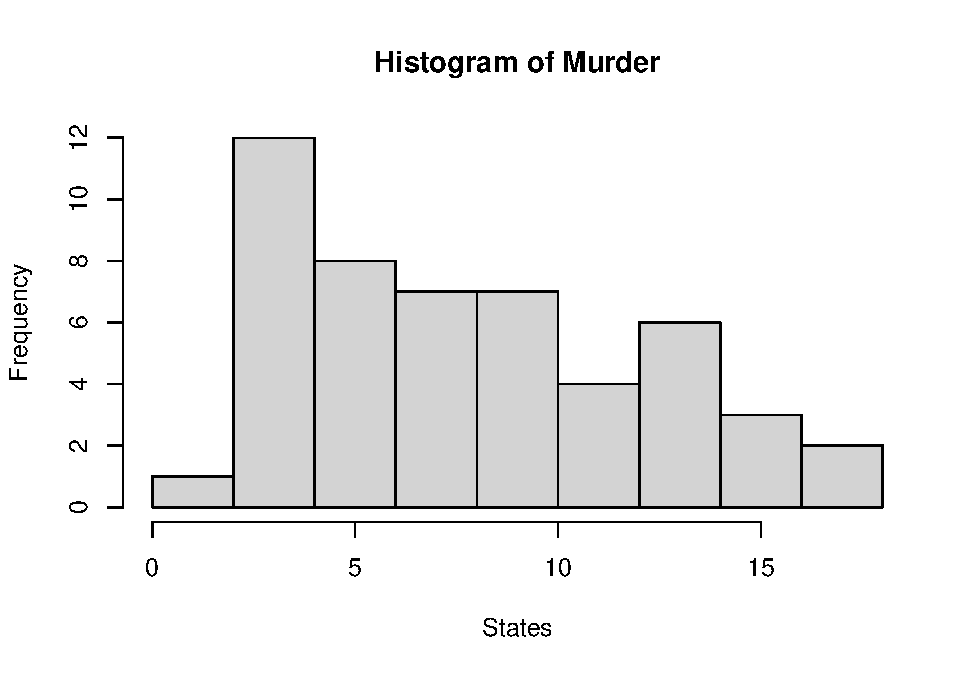
\includegraphics{Journal_files/figure-latex/unnamed-chunk-5-1.pdf}

\hypertarget{problem-6}{%
\subsubsection{Problem 6}\label{problem-6}}

Please summarize \texttt{Murder} quantitatively. What are its mean and
median? What is the difference between mean and median? What is a
quartile, and why do you think R gives you the 1st Qu. and 3rd Qu.?

\begin{Shaded}
\begin{Highlighting}[]
  \FunctionTok{summary}\NormalTok{(dat}\SpecialCharTok{$}\NormalTok{Murder)}
\end{Highlighting}
\end{Shaded}

\begin{verbatim}
##    Min. 1st Qu.  Median    Mean 3rd Qu.    Max. 
##   0.800   4.075   7.250   7.788  11.250  17.400
\end{verbatim}

Min. 1st Qu. Median Mean 3rd Qu. Max. 0.800 4.075 7.250 7.788 11.250
17.400

The mean is 7.788 and the median and 7.250. The mean is the average of
the dataset while the median gives us a central value of our dataset. A
quartile tells us the variability around the median. So the 1st and 3rd
quartiles show us the variability before the median is reached and after
the median is reached. R gives us this data to show us where it might be
more or less skewed.

\hypertarget{problem-7}{%
\subsubsection{Problem 7}\label{problem-7}}

Repeat the same steps you followed for \texttt{Murder}, for the
variables \texttt{Assault} and \texttt{Rape}. Now plot all three
histograms together. You can do this by using the command
\texttt{par(mfrow=c(3,1))} and then plotting each of the three.

Answer (for data on the other two variables) : For assaults, the mean is
170.8 and the median and 159.0.

For rapes, the mean is 21.23 and the median and 20.10.

\begin{Shaded}
\begin{Highlighting}[]
\FunctionTok{summary}\NormalTok{(dat}\SpecialCharTok{$}\NormalTok{Murder)}
\end{Highlighting}
\end{Shaded}

\begin{verbatim}
##    Min. 1st Qu.  Median    Mean 3rd Qu.    Max. 
##   0.800   4.075   7.250   7.788  11.250  17.400
\end{verbatim}

\begin{Shaded}
\begin{Highlighting}[]
\FunctionTok{summary}\NormalTok{(dat}\SpecialCharTok{$}\NormalTok{Assault)}
\end{Highlighting}
\end{Shaded}

\begin{verbatim}
##    Min. 1st Qu.  Median    Mean 3rd Qu.    Max. 
##    45.0   109.0   159.0   170.8   249.0   337.0
\end{verbatim}

\begin{Shaded}
\begin{Highlighting}[]
\FunctionTok{summary}\NormalTok{(dat}\SpecialCharTok{$}\NormalTok{Rape)}
\end{Highlighting}
\end{Shaded}

\begin{verbatim}
##    Min. 1st Qu.  Median    Mean 3rd Qu.    Max. 
##    7.30   15.07   20.10   21.23   26.18   46.00
\end{verbatim}

\begin{Shaded}
\begin{Highlighting}[]
\FunctionTok{par}\NormalTok{(}\AttributeTok{mfrow=}\FunctionTok{c}\NormalTok{(}\DecValTok{3}\NormalTok{,}\DecValTok{1}\NormalTok{))}
\FunctionTok{hist}\NormalTok{(dat}\SpecialCharTok{$}\NormalTok{Assault, }\AttributeTok{main =} \StringTok{"Histogram of Assault"}\NormalTok{, }\AttributeTok{xlab =} \StringTok{"States"}\NormalTok{)}
\FunctionTok{hist}\NormalTok{(dat}\SpecialCharTok{$}\NormalTok{Murder, }\AttributeTok{main =} \StringTok{"Histogram of Murder"}\NormalTok{, }\AttributeTok{xlab =} \StringTok{"States"}\NormalTok{)}
\FunctionTok{hist}\NormalTok{(dat}\SpecialCharTok{$}\NormalTok{Rape, }\AttributeTok{main =} \StringTok{"Histogram of Rape"}\NormalTok{, }\AttributeTok{xlab =} \StringTok{"States"}\NormalTok{)}
\end{Highlighting}
\end{Shaded}

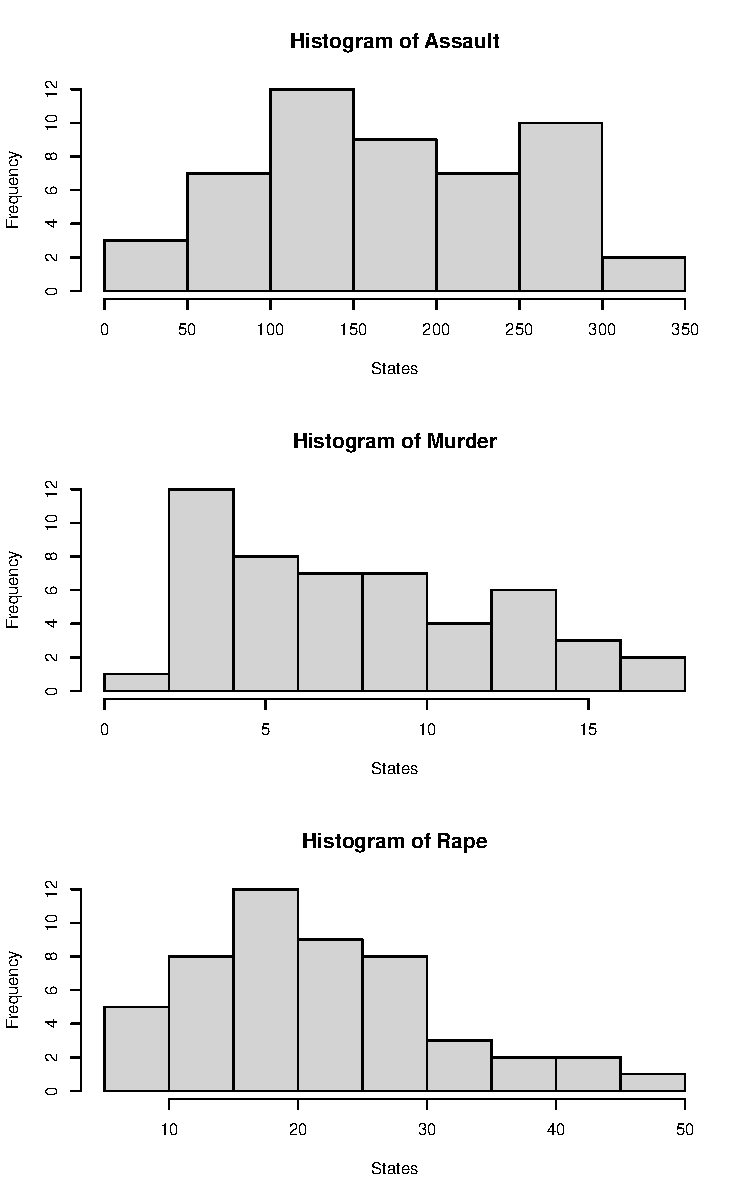
\includegraphics{Journal_files/figure-latex/unnamed-chunk-7-1.pdf}

What does the command par do, in your own words (you can look this up by
asking R \texttt{?par})?

Answer: It helps us combine multiple plots that we created into one big
vertical plot.

What can you learn from plotting the histograms together?

Answer: We can see the correlation between the data. If there are some
points where there is a peak at the same time then we can generalize and
say that state could be more dangerous than others. This could work
likewise for the converse situation.

\hypertarget{problem-8}{%
\subsubsection{Problem 8}\label{problem-8}}

In the console below (not in text), type
\texttt{install.packages("maps")} and press Enter, and then type
\texttt{install.packages("ggplot2")} and press Enter. This will install
the packages so you can load the libraries.

Run this code:

\begin{Shaded}
\begin{Highlighting}[]
\FunctionTok{library}\NormalTok{(}\StringTok{\textquotesingle{}maps\textquotesingle{}}\NormalTok{) }
\FunctionTok{library}\NormalTok{(}\StringTok{\textquotesingle{}ggplot2\textquotesingle{}}\NormalTok{) }

\FunctionTok{ggplot}\NormalTok{(dat, }\FunctionTok{aes}\NormalTok{(}\AttributeTok{map\_id=}\NormalTok{state, }\AttributeTok{fill=}\NormalTok{Murder)) }\SpecialCharTok{+} 
  \FunctionTok{geom\_map}\NormalTok{(}\AttributeTok{map=}\FunctionTok{map\_data}\NormalTok{(}\StringTok{"state"}\NormalTok{)) }\SpecialCharTok{+} 
  \FunctionTok{expand\_limits}\NormalTok{(}\AttributeTok{x=}\FunctionTok{map\_data}\NormalTok{(}\StringTok{"state"}\NormalTok{)}\SpecialCharTok{$}\NormalTok{long, }\AttributeTok{y=}\FunctionTok{map\_data}\NormalTok{(}\StringTok{"state"}\NormalTok{)}\SpecialCharTok{$}\NormalTok{lat)}
\end{Highlighting}
\end{Shaded}

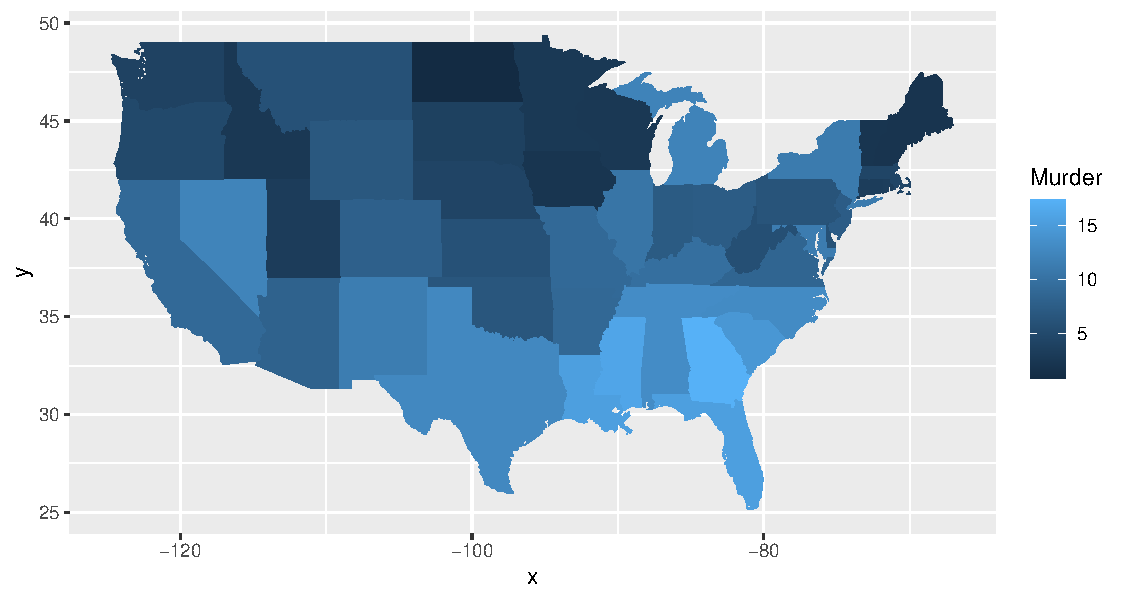
\includegraphics{Journal_files/figure-latex/unnamed-chunk-8-1.pdf}

What does this code do? Explain what each line is doing.

Answer: The first two lines import the libraries map and ggplot2. Line
154 imports dat wants to define the map id of states with murder. The
second line is filling out map with state data.The third line maps it
out in a x and y axis so we can see the data in states.

\hypertarget{assignment-2}{%
\section{Assignment 2}\label{assignment-2}}

\hypertarget{problem-1-load-data}{%
\subsection{Problem 1: Load data}\label{problem-1-load-data}}

Set your working directory to the folder where you downloaded the data.

\begin{Shaded}
\begin{Highlighting}[]
\FunctionTok{setwd}\NormalTok{(}\StringTok{"/Users/akshatshah/Desktop/upenn/crim250/LabJournal"}\NormalTok{)}
\end{Highlighting}
\end{Shaded}

\hypertarget{read-the-data}{%
\subsection{Read the data}\label{read-the-data}}

\begin{Shaded}
\begin{Highlighting}[]
\NormalTok{dat }\OtherTok{\textless{}{-}} \FunctionTok{read.csv}\NormalTok{(}\AttributeTok{file =} \StringTok{\textquotesingle{}dat.nsduh.small.1.csv\textquotesingle{}}\NormalTok{)}
\end{Highlighting}
\end{Shaded}

What are the dimensions of the dataset?

\begin{Shaded}
\begin{Highlighting}[]
\FunctionTok{dim}\NormalTok{(dat)}
\end{Highlighting}
\end{Shaded}

\begin{verbatim}
## [1] 171   7
\end{verbatim}

Answer: There are 171 rows and 7 columns in this dataset.

\begin{Shaded}
\begin{Highlighting}[]
\FunctionTok{names}\NormalTok{(dat)}
\end{Highlighting}
\end{Shaded}

\begin{verbatim}
## [1] "mjage"     "cigage"    "iralcage"  "age2"      "sexatract" "speakengl"
## [7] "irsex"
\end{verbatim}

\hypertarget{problem-2-variables}{%
\subsection{Problem 2: Variables}\label{problem-2-variables}}

Describe the variables in the dataset.

The variables are mjage, ciage, iralcage, age2, sexatract, speakengl,
and irsex. They each tell us different things. Mjage tells how old
someone was when they first starting using marijuana. Ciage tells how
old someone was when they first starting smoking cigs every day.
iralcage tells how old someone was when they tried alcohol. age2 tells
us hpw old the person currently is. However, this gives us a range
because a person could have changes their choice based on previous
responses and the questions they say. Irsex tells us their gender.
sexatract tells us describes their attraction/sexuality. speakengl tells
how well the individual speaks english.

What is this dataset about? Who collected the data, what kind of sample
is it, and what was the purpose of generating the data?

This dataset is a survey about national drug use and health. The data is
sponsored by the United States Health and Human Services. The sample is
a scientific random sample of household addresses. This data gives us a
state and nationwide statistics on drug use. This information is used to
help with prevention, trend studies, and inform public health policy.

\hypertarget{problem-3-age-and-gender}{%
\subsection{Problem 3: Age and gender}\label{problem-3-age-and-gender}}

What is the age distribution of the sample like? Make sure you read the
codebook to know what the variable values mean.

The age distribution is more towards the 13-17 year old range. However,
when we look at this data we should understand that it can be more of a
range since participants could change their answers based on the
decisions on they made or what they see fit.

Do you think this age distribution representative of the US population?
Why or why not?

I believe this data not a good representative of the US population. We
are looking at a younger population that makes up around 35\% of the age
distribution. So we are leaving out a large majority that can help us
see more trends.

Is the sample balanced in terms of gender? If not, are there more
females or males?

I believe this data is pretty balanced. There is a pretty even
distribution but for some of the ages we can see that there is a clear
majority like for 17.

Use this code to draw a stacked bar plot to view the relationship
between sex and age. What can you conclude from this plot?

\begin{Shaded}
\begin{Highlighting}[]
\NormalTok{tab.agesex }\OtherTok{\textless{}{-}} \FunctionTok{table}\NormalTok{(dat}\SpecialCharTok{$}\NormalTok{irsex, dat}\SpecialCharTok{$}\NormalTok{age2)}

\FunctionTok{barplot}\NormalTok{(tab.agesex,}
        \AttributeTok{main =} \StringTok{"Stacked barchart"}\NormalTok{,}
        \AttributeTok{xlab =} \StringTok{"Age category"}\NormalTok{, }\AttributeTok{ylab =} \StringTok{"Frequency"}\NormalTok{,}
        \AttributeTok{legend.text =} \FunctionTok{rownames}\NormalTok{(tab.agesex),}
        \AttributeTok{beside =} \ConstantTok{FALSE}\NormalTok{) }\CommentTok{\# Stacked bars (default)}
\end{Highlighting}
\end{Shaded}

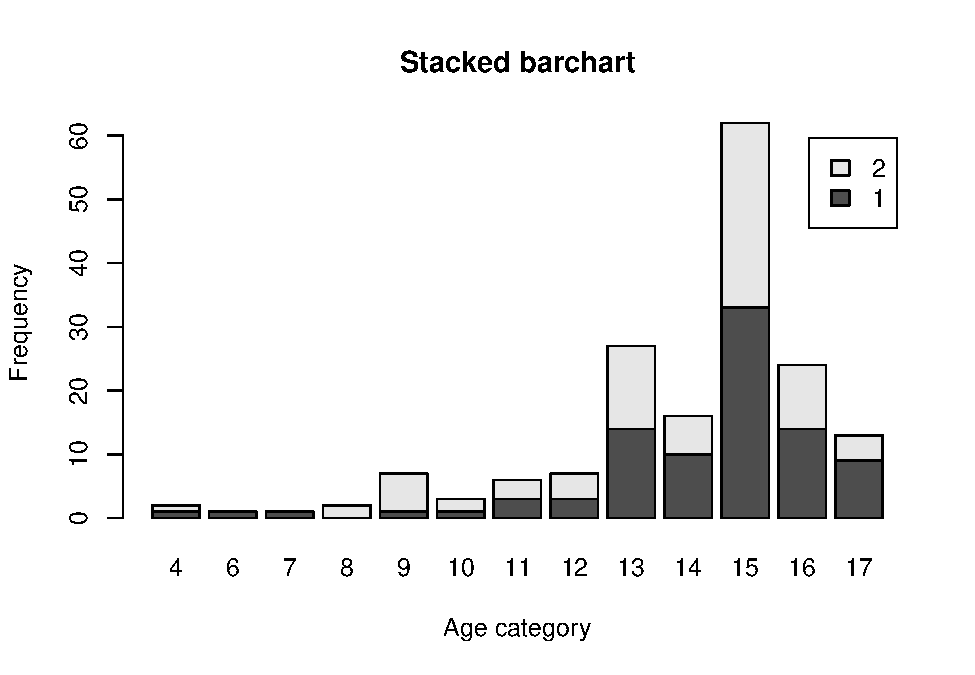
\includegraphics{Journal_files/figure-latex/unnamed-chunk-13-1.pdf}

\hypertarget{problem-4-substance-use}{%
\subsection{Problem 4: Substance use}\label{problem-4-substance-use}}

For which of the three substances included in the dataset (marijuana,
alcohol, and cigarettes) do individuals tend to use the substance
earlier?

\begin{Shaded}
\begin{Highlighting}[]
\FunctionTok{summary}\NormalTok{(dat)}
\end{Highlighting}
\end{Shaded}

\begin{verbatim}
##      mjage           cigage         iralcage          age2      
##  Min.   : 7.00   Min.   :10.00   Min.   : 5.00   Min.   : 4.00  
##  1st Qu.:14.00   1st Qu.:15.00   1st Qu.:13.00   1st Qu.:13.00  
##  Median :16.00   Median :17.00   Median :15.00   Median :15.00  
##  Mean   :15.99   Mean   :17.65   Mean   :14.95   Mean   :13.98  
##  3rd Qu.:17.50   3rd Qu.:19.00   3rd Qu.:17.00   3rd Qu.:15.00  
##  Max.   :35.00   Max.   :50.00   Max.   :23.00   Max.   :17.00  
##    sexatract       speakengl        irsex      
##  Min.   : 1.00   Min.   :1.00   Min.   :1.000  
##  1st Qu.: 1.00   1st Qu.:1.00   1st Qu.:1.000  
##  Median : 1.00   Median :1.00   Median :1.000  
##  Mean   : 3.07   Mean   :1.07   Mean   :1.468  
##  3rd Qu.: 1.00   3rd Qu.:1.00   3rd Qu.:2.000  
##  Max.   :99.00   Max.   :3.00   Max.   :2.000
\end{verbatim}

Looking at the summary of the data, we can see on average what is used
earlier on. Alcohol seems to be used the earliest at an average of
14.95. Then it is mjage at 15.99 Finally, it is cigage at 17.65.

\hypertarget{problem-5-sexual-attraction}{%
\subsection{Problem 5: Sexual
attraction}\label{problem-5-sexual-attraction}}

What does the distribution of sexual attraction look like? Is this what
you expected?

\begin{Shaded}
\begin{Highlighting}[]
\FunctionTok{table}\NormalTok{(dat}\SpecialCharTok{$}\NormalTok{sexatract)}
\end{Highlighting}
\end{Shaded}

\begin{verbatim}
## 
##   1   2   3   4   5   6  99 
## 136  16   9   3   3   1   3
\end{verbatim}

We see that the largest amount of people (136) chose 1. Yes, this is
what I expected since it is the norm to be heterosexual.

What is the distribution of sexual attraction by gender?

\begin{Shaded}
\begin{Highlighting}[]
\FunctionTok{table}\NormalTok{(dat}\SpecialCharTok{$}\NormalTok{sexatract, dat}\SpecialCharTok{$}\NormalTok{irsex)}
\end{Highlighting}
\end{Shaded}

\begin{verbatim}
##     
##       1  2
##   1  82 54
##   2   3 13
##   3   0  9
##   4   1  2
##   5   2  1
##   6   1  0
##   99  2  1
\end{verbatim}

By gender, the distribution is the same in that the majority of both
gender are attracted to the opposite gender. However, more females chose
other options.

\hypertarget{problem-6-english-speaking}{%
\subsection{Problem 6: English
speaking}\label{problem-6-english-speaking}}

What does the distribution of English speaking look like in the sample?
Is this what you might expect for a random sample of the US population?

\begin{Shaded}
\begin{Highlighting}[]
\FunctionTok{table}\NormalTok{(dat}\SpecialCharTok{$}\NormalTok{speakengl)}
\end{Highlighting}
\end{Shaded}

\begin{verbatim}
## 
##   1   2   3 
## 161   8   2
\end{verbatim}

The majority of people chose that they speak english very well. And
there were very few who chose well and not well (10 total). This is
probably what I would expect since it is the dominant language.

Are there more English speaker females or males?

\begin{Shaded}
\begin{Highlighting}[]
\FunctionTok{table}\NormalTok{(dat}\SpecialCharTok{$}\NormalTok{speakengl, dat}\SpecialCharTok{$}\NormalTok{irsex)}
\end{Highlighting}
\end{Shaded}

\begin{verbatim}
##    
##      1  2
##   1 84 77
##   2  7  1
##   3  0  2
\end{verbatim}

There are more English speakers who are male than female.

\hypertarget{exam-1}{%
\section{Exam 1}\label{exam-1}}

\hypertarget{instructions}{%
\subsection{Instructions}\label{instructions}}

\begin{enumerate}
\def\labelenumi{\alph{enumi}.}
\item
  Create a folder in your computer (a good place would be under Crim
  250, Exams).
\item
  Download the dataset from the Canvas website
  (fatal-police-shootings-data.csv) onto that folder, and save your Exam
  1.Rmd file in the same folder.
\item
  Download the README.md file. This is the codebook.
\item
  Load the data into an R data frame.
\end{enumerate}

\begin{Shaded}
\begin{Highlighting}[]
\NormalTok{dat }\OtherTok{\textless{}{-}} \FunctionTok{read.csv}\NormalTok{(}\AttributeTok{file =} \StringTok{"Crim 250 {-} Exam 1/fatal{-}police{-}shootings{-}data.csv"}\NormalTok{)}
\end{Highlighting}
\end{Shaded}

\hypertarget{problem-1-10-points}{%
\subsection{Problem 1 (10 points)}\label{problem-1-10-points}}

\begin{enumerate}
\def\labelenumi{\alph{enumi}.}
\tightlist
\item
  Describe the dataset. This is the source:
  \url{https://github.com/washingtonpost/data-police-shootings} . Write
  two sentences (max.) about this.
\end{enumerate}

This is a dataset that is compiled by the Washington Post of victims of
fatal police shootings. At each row, we are given a victim's name and
data on the situation that was at hand.

\begin{enumerate}
\def\labelenumi{\alph{enumi}.}
\setcounter{enumi}{1}
\tightlist
\item
  How many observations are there in the data frame?
\end{enumerate}

\begin{Shaded}
\begin{Highlighting}[]
\FunctionTok{dim}\NormalTok{((dat))}
\end{Highlighting}
\end{Shaded}

\begin{verbatim}
## [1] 6594   17
\end{verbatim}

We know there are 6594 rows and 17 columns. We know that the number of
observations are the number of rows. Therefore there are 6593
observations (not including the first row since this is the title of the
columns).

\begin{enumerate}
\def\labelenumi{\alph{enumi}.}
\setcounter{enumi}{2}
\tightlist
\item
  Look at the names of the variables in the data frame. Describe what
  ``body\_camera'', ``flee'', and ``armed'' represent, according to the
  codebook. Again, only write one sentence (max) per variable.
\end{enumerate}

\begin{Shaded}
\begin{Highlighting}[]
\FunctionTok{names}\NormalTok{(dat)}
\end{Highlighting}
\end{Shaded}

\begin{verbatim}
##  [1] "id"                      "name"                   
##  [3] "date"                    "manner_of_death"        
##  [5] "armed"                   "age"                    
##  [7] "gender"                  "race"                   
##  [9] "city"                    "state"                  
## [11] "signs_of_mental_illness" "threat_level"           
## [13] "flee"                    "body_camera"            
## [15] "longitude"               "latitude"               
## [17] "is_geocoding_exact"
\end{verbatim}

Body camera is a variable that is telling us if an officer was wearing a
body camera and if it was recording what happened.

Flee is a variable that was indicating if the victim was moving away,
and if they were fleeing this tells us by what method.

Armed is a variable that tells if the officer believe they had some tool
that could inflict damage.

\begin{enumerate}
\def\labelenumi{\alph{enumi}.}
\setcounter{enumi}{3}
\tightlist
\item
  What are three weapons that you are surprised to find in the ``armed''
  variable? Make a table of the values in ``armed'' to see the options.
\end{enumerate}

\begin{Shaded}
\begin{Highlighting}[]
\FunctionTok{table}\NormalTok{(dat}\SpecialCharTok{$}\NormalTok{armed)}
\end{Highlighting}
\end{Shaded}

\begin{verbatim}
## 
##                                                   air conditioner 
##                              207                                1 
##                       air pistol                   Airsoft pistol 
##                                1                                3 
##                               ax                         barstool 
##                               24                                1 
##                     baseball bat          baseball bat and bottle 
##                               20                                1 
## baseball bat and fireplace poker           baseball bat and knife 
##                                1                                1 
##                            baton                           BB gun 
##                                6                               15 
##               BB gun and vehicle                     bean-bag gun 
##                                1                                1 
##                      beer bottle                       binoculars 
##                                3                                1 
##                     blunt object                           bottle 
##                                5                                1 
##                    bow and arrow                       box cutter 
##                                1                               13 
##                            brick              car, knife and mace 
##                                2                                1 
##                          carjack                            chain 
##                                1                                3 
##                        chain saw                         chainsaw 
##                                2                                1 
##                            chair              claimed to be armed 
##                                4                                1 
##               contractor's level                   cordless drill 
##                                1                                1 
##                         crossbow                          crowbar 
##                                9                                5 
##                        fireworks                         flagpole 
##                                1                                1 
##                       flashlight                      garden tool 
##                                2                                2 
##                      glass shard                          grenade 
##                                4                                1 
##                              gun                      gun and car 
##                             3798                               12 
##                    gun and knife                  gun and machete 
##                               22                                3 
##                    gun and sword                  gun and vehicle 
##                                1                               17 
##              guns and explosives                           hammer 
##                                3                               18 
##                       hand torch                          hatchet 
##                                1                               14 
##                  hatchet and gun                         ice pick 
##                                2                                1 
##                incendiary device                            knife 
##                                2                              955 
##                knife and vehicle                 lawn mower blade 
##                                1                                2 
##                          machete                  machete and gun 
##                               51                                1 
##                     meat cleaver                  metal hand tool 
##                                6                                2 
##                     metal object                       metal pipe 
##                                5                               16 
##                       metal pole                       metal rake 
##                                4                                1 
##                      metal stick                       microphone 
##                                3                                1 
##                       motorcycle                         nail gun 
##                                1                                1 
##                              oar                       pellet gun 
##                                1                                3 
##                              pen                     pepper spray 
##                                1                                2 
##                         pick-axe                    piece of wood 
##                                4                                7 
##                             pipe                        pitchfork 
##                                7                                2 
##                             pole                   pole and knife 
##                                3                                2 
##                  railroad spikes                             rock 
##                                1                                7 
##                    samurai sword                         scissors 
##                                4                                9 
##                      screwdriver                     sharp object 
##                               16                               14 
##                           shovel                            spear 
##                                7                                2 
##                          stapler              straight edge razor 
##                                1                                5 
##                            sword                            Taser 
##                               23                               34 
##                        tire iron                       toy weapon 
##                                4                              226 
##                          unarmed                     undetermined 
##                              421                              188 
##                   unknown weapon                          vehicle 
##                               82                              213 
##                  vehicle and gun              vehicle and machete 
##                                8                                1 
##                    walking stick                       wasp spray 
##                                1                                1 
##                           wrench 
##                                1
\end{verbatim}

I am suprised to see pen, binoculars, and contractor's level.

\hypertarget{problem-2-10-points}{%
\subsection{Problem 2 (10 points)}\label{problem-2-10-points}}

\begin{enumerate}
\def\labelenumi{\alph{enumi}.}
\tightlist
\item
  Describe the age distribution of the sample. Is this what you would
  expect to see?
\end{enumerate}

\begin{Shaded}
\begin{Highlighting}[]
\FunctionTok{hist}\NormalTok{(dat}\SpecialCharTok{$}\NormalTok{age, }\AttributeTok{main =} \StringTok{"Histogram of Age Distribution"}\NormalTok{, }\AttributeTok{xlab =} \StringTok{"Age (in years)"}\NormalTok{, }\AttributeTok{xlim =} \FunctionTok{c}\NormalTok{(}\DecValTok{0}\NormalTok{, }\DecValTok{100}\NormalTok{))}
\end{Highlighting}
\end{Shaded}

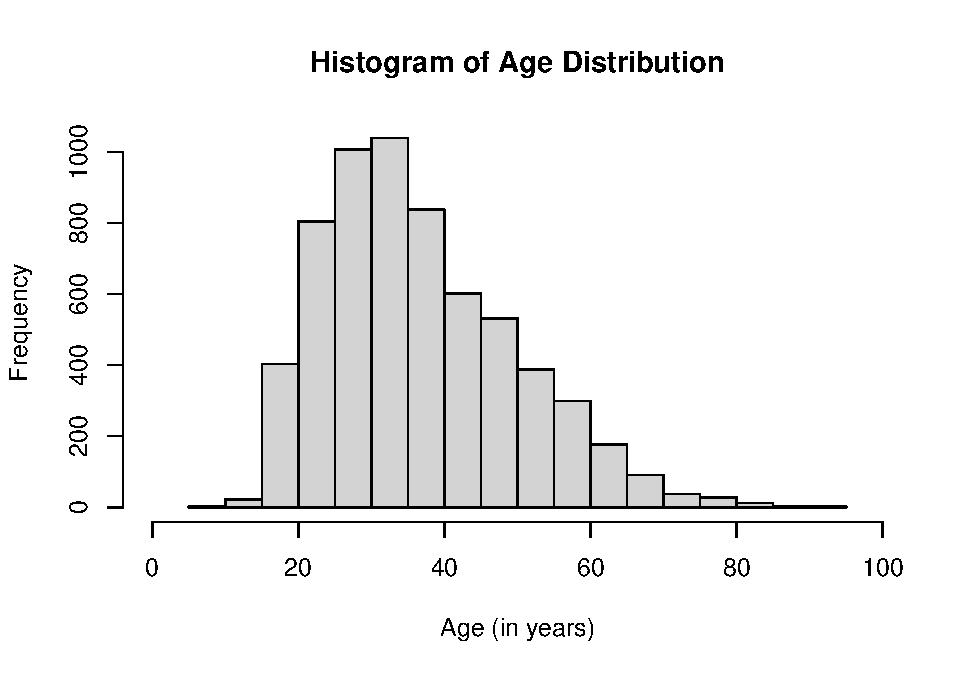
\includegraphics{Journal_files/figure-latex/unnamed-chunk-23-1.pdf}

This distribution is skewed to the right. This isn't exactly what I
expected, (I thought it would be skewed even more to the right.) because
I believed that victims would be a lot younger.

\begin{enumerate}
\def\labelenumi{\alph{enumi}.}
\setcounter{enumi}{1}
\tightlist
\item
  To understand the center of the age distribution, would you use a mean
  or a median, and why? Find the one you picked.
\end{enumerate}

\begin{Shaded}
\begin{Highlighting}[]
\FunctionTok{summary}\NormalTok{(dat}\SpecialCharTok{$}\NormalTok{age)}
\end{Highlighting}
\end{Shaded}

\begin{verbatim}
##    Min. 1st Qu.  Median    Mean 3rd Qu.    Max.    NA's 
##    6.00   27.00   35.00   37.12   45.00   91.00     308
\end{verbatim}

I would use mean to understand the center of the age distribution
because I don't believe there are enough outliers/extremes that would
skew this result substantially. The mean gives us an average over our
data. We can see that the average age of victims for police fatal
shootings were 37.12 years old.

\begin{enumerate}
\def\labelenumi{\alph{enumi}.}
\setcounter{enumi}{2}
\tightlist
\item
  Describe the gender distribution of the sample. Do you find this
  surprising?
\end{enumerate}

\begin{Shaded}
\begin{Highlighting}[]
\FunctionTok{table}\NormalTok{(dat}\SpecialCharTok{$}\NormalTok{gender)}
\end{Highlighting}
\end{Shaded}

\begin{verbatim}
## 
##         F    M 
##    3  293 6298
\end{verbatim}

Within this dataset, there are significantly more men than women (6005
more). This is not surprising because statistics have shown that men
have been higher arrest rate than women. Since men have a higher arrest
rate than women and more encounters with police, I expected there to be
more men than women within this dataset. Additonally, there were 3 blank
indexes for this data and it was not taken into account for the
calculations above since it is inconclusive.

\hypertarget{problem-3-10-points}{%
\subsection{Problem 3 (10 points)}\label{problem-3-10-points}}

\begin{enumerate}
\def\labelenumi{\alph{enumi}.}
\tightlist
\item
  How many police officers had a body camera, according to news reports?
  What proportion is this of all the incidents in the data? Are you
  surprised that it is so high or low?
\end{enumerate}

\begin{Shaded}
\begin{Highlighting}[]
\FunctionTok{table}\NormalTok{(dat}\SpecialCharTok{$}\NormalTok{body\_camera)}
\end{Highlighting}
\end{Shaded}

\begin{verbatim}
## 
## False  True 
##  5684   910
\end{verbatim}

Only 910 officers had a body camera according to this dataset. This
means that only 14\% of incidents had a body camera. This is extremely
suprising that is so low because people are losing their lives and a
proportion of officers have no concrete evidence of the situation due to
no body camera.

\begin{enumerate}
\def\labelenumi{\alph{enumi}.}
\setcounter{enumi}{1}
\tightlist
\item
  In how many of the incidents was the victim fleeing? What proportion
  is this of the total number of incidents in the data? Is this what you
  would expect?
\end{enumerate}

\begin{Shaded}
\begin{Highlighting}[]
\FunctionTok{table}\NormalTok{(dat}\SpecialCharTok{$}\NormalTok{flee)}
\end{Highlighting}
\end{Shaded}

\begin{verbatim}
## 
##                     Car        Foot Not fleeing       Other 
##         491        1058         845        3952         248
\end{verbatim}

Out of 6103 incidents that recorded something in the fleeing category,
2151 victims were fleeing. This means about 35\% of people who were a
victim of a fatal police shooting were fleeing. I suspected a larger
proportion of people were fleeing, but this dataset refutes that idea.
Additionally, there is 491 indexes of data that are blank for fleeing,
so this was removed from the total number of incidents and the
proportion since it is inconclusive.

\hypertarget{problem-4-10-points---answer-only-one-of-these-a-or-b.}{%
\subsection{Problem 4 (10 points) - Answer only one of these (a or
b).}\label{problem-4-10-points---answer-only-one-of-these-a-or-b.}}

\begin{enumerate}
\def\labelenumi{\alph{enumi}.}
\tightlist
\item
  Describe the relationship between the variables ``body camera'' and
  ``flee'' using a stacked barplot. What can you conclude from this
  relationship?
\end{enumerate}

\emph{Hint 1: The categories along the x-axis are the options for
``flee'', each bar contains information about whether the police officer
had a body camera (vertically), and the height along the y-axis shows
the frequency of that category).}

\emph{Hint 2: Also, if you are unsure about the syntax for barplot, run
?barplot in R and see some examples at the bottom of the documentation.
This is usually a good way to look up the syntax of R code. You can also
Google it.}

\textbf{Your answer here.}

\begin{enumerate}
\def\labelenumi{\alph{enumi}.}
\setcounter{enumi}{1}
\tightlist
\item
  Describe the relationship between age and race by using a boxplot.
  What can you conclude from this relationship?
\end{enumerate}

\emph{Hint 1: The categories along the x-axis are the race categories
and the height along the y-axis is age.}

\emph{Hint 2: Also, if you are unsure about the syntax for boxplot, run
?boxplot in R and see some examples at the bottom of the documentation.
This is usually a good way to look up the syntax of R code. You can also
Google it.}

\begin{Shaded}
\begin{Highlighting}[]
\FunctionTok{boxplot}\NormalTok{(dat}\SpecialCharTok{$}\NormalTok{age}\SpecialCharTok{\textasciitilde{}}\FunctionTok{factor}\NormalTok{(dat}\SpecialCharTok{$}\NormalTok{race), }\AttributeTok{ylab =} \StringTok{"Age"}\NormalTok{, }\AttributeTok{xlab =} \StringTok{"Race"}\NormalTok{)}
\end{Highlighting}
\end{Shaded}

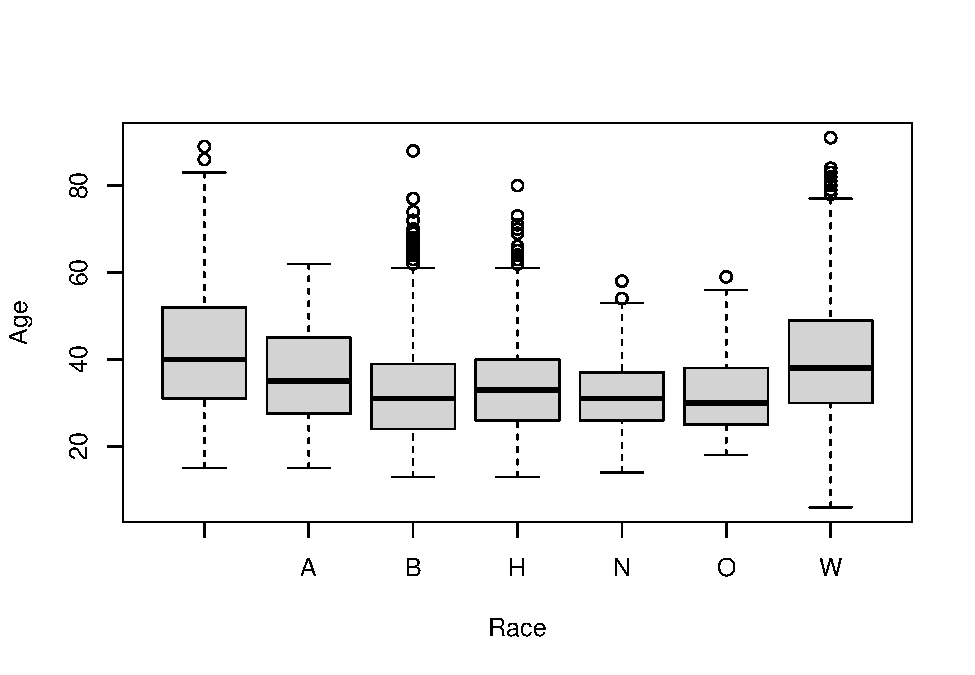
\includegraphics{Journal_files/figure-latex/unnamed-chunk-29-1.pdf}

We see from the data that some races have a slightly lower mean age than
others. For examples, the mean age for white people looks to be around
40, while the mean age for black people seems to be about 35.
Additionally, some races have a lot more outliers than others. For
example, asian people have no outliers while black people have a lot of
outliers. It is hard to make a concrete conclusion based on this
relationship, but we can observe that there are clear small differences
that we can observe (as stated above) from the different races and their
ages. Furthermore, the first category simple represent people who did
not have a specified age (left blank in the dataset). I did not omit
this data because I think it could still be important to see this in
relation to the other data.

\hypertarget{extra-credit-10-points}{%
\subsection{Extra credit (10 points)}\label{extra-credit-10-points}}

\begin{enumerate}
\def\labelenumi{\alph{enumi}.}
\tightlist
\item
  What does this code tell us?
\end{enumerate}

\begin{Shaded}
\begin{Highlighting}[]
\NormalTok{mydates }\OtherTok{\textless{}{-}} \FunctionTok{as.Date}\NormalTok{(dat}\SpecialCharTok{$}\NormalTok{date)}
\FunctionTok{head}\NormalTok{(mydates)}
\NormalTok{(mydates[}\FunctionTok{length}\NormalTok{(mydates)] }\SpecialCharTok{{-}}\NormalTok{ mydates[}\DecValTok{1}\NormalTok{])}
\end{Highlighting}
\end{Shaded}

This data tells us how long it has been since the first entry within
this dataset to the most recent entry within the dataset. We are taking
the first index because the 0th index states the name of each column,
and we are taking the last index to get the last entry. The difference
is 2458 days which is about 6.7 years. This makes sense because this
dataset was created in 2015 and we are about 6 and 3/4 years from this
time.

\begin{enumerate}
\def\labelenumi{\alph{enumi}.}
\setcounter{enumi}{1}
\tightlist
\item
  On Friday, a new report was published that was described as follows by
  The Guardian: ``More than half of US police killings are mislabelled
  or not reported, study finds.'' Without reading this article now (due
  to limited time), why do you think police killings might be
  mislabelled or underreported?
\end{enumerate}

I believe this is because of bias. Police who have been apart of police
killings are going to defend themselves. In order to do so, they might
underreport or mislabel the incident in order to save face and justify
the actions they took. Additionally, co workers of police who have been
apart of such an incident may look to defend each other building even
more of a bias.

\begin{enumerate}
\def\labelenumi{\alph{enumi}.}
\setcounter{enumi}{2}
\tightlist
\item
  Regarding missing values in problem 4, do you see any? If so, do you
  think that's all that's missing from the data?
\end{enumerate}

In problem 4, there were clear missing values (race was not defined). I
believe there is more missing from the data. If we were to look closer
into the data we can see that sometimes, for example, gender isn't
specified. Additionally, another data that has missing values is fleeing
(491 are blank).

\hypertarget{exam-2}{%
\section{Exam 2}\label{exam-2}}

\hypertarget{instructions-1}{%
\subsection{Instructions}\label{instructions-1}}

\begin{enumerate}
\def\labelenumi{\alph{enumi}.}
\item
  Create a folder in your computer (a good place would be under Crim
  250, Exams).
\item
  Download the dataset from the Canvas website (sim.data.csv) onto that
  folder, and save your Exam 2.Rmd file in the same folder.
\item
  Data description: This dataset provides (simulated) data about 200
  police departments in one year. It contains information about the
  funding received by the department as well as incidents of police
  brutality. Suppose this dataset (sim.data.csv) was collected by
  researchers to answer this question: \textbf{``Does having more
  funding in a police department lead to fewer incidents of police
  brutality?''}
\item
  Codebook:
\end{enumerate}

\begin{itemize}
\tightlist
\item
  funds: How much funding the police department received in that year in
  millions of dollars.
\item
  po.brut: How many incidents of police brutality were reported by the
  department that year.
\item
  po.dept.code: Police department code
\end{itemize}

\hypertarget{problem-1-eda-10-points}{%
\subsection{Problem 1: EDA (10 points)}\label{problem-1-eda-10-points}}

Describe the dataset and variables. Perform exploratory data analysis
for the two variables of interest: funds and po.brut.

\begin{Shaded}
\begin{Highlighting}[]
\NormalTok{dat }\OtherTok{\textless{}{-}} \FunctionTok{read.csv}\NormalTok{(}\AttributeTok{file =} \StringTok{\textquotesingle{}sim.data.csv\textquotesingle{}}\NormalTok{)}
\FunctionTok{names}\NormalTok{(dat)}
\end{Highlighting}
\end{Shaded}

\begin{verbatim}
## [1] "po.dept.code" "funds"        "po.brut"
\end{verbatim}

\begin{Shaded}
\begin{Highlighting}[]
\FunctionTok{summary}\NormalTok{(dat)}
\end{Highlighting}
\end{Shaded}

\begin{verbatim}
##   po.dept.code        funds          po.brut     
##  Min.   :  1.00   Min.   :21.40   Min.   : 0.00  
##  1st Qu.: 50.75   1st Qu.:51.67   1st Qu.:14.00  
##  Median :100.50   Median :59.75   Median :19.00  
##  Mean   :100.50   Mean   :61.04   Mean   :18.14  
##  3rd Qu.:150.25   3rd Qu.:72.17   3rd Qu.:22.00  
##  Max.   :200.00   Max.   :99.70   Max.   :29.00
\end{verbatim}

\begin{Shaded}
\begin{Highlighting}[]
\FunctionTok{dim}\NormalTok{(dat)}
\end{Highlighting}
\end{Shaded}

\begin{verbatim}
## [1] 200   3
\end{verbatim}

\begin{Shaded}
\begin{Highlighting}[]
\FunctionTok{plot}\NormalTok{(dat}\SpecialCharTok{$}\NormalTok{funds, dat}\SpecialCharTok{$}\NormalTok{po.brut,  }\AttributeTok{main=}\StringTok{"Relationship between Police Department Funding (in millions) and Police Bruality (per year)"}\NormalTok{, }\AttributeTok{xlab=}\StringTok{"Amount of funding"}\NormalTok{, }\AttributeTok{ylab=}\StringTok{"Number of police brutality incidences per year"}\NormalTok{)}
\end{Highlighting}
\end{Shaded}

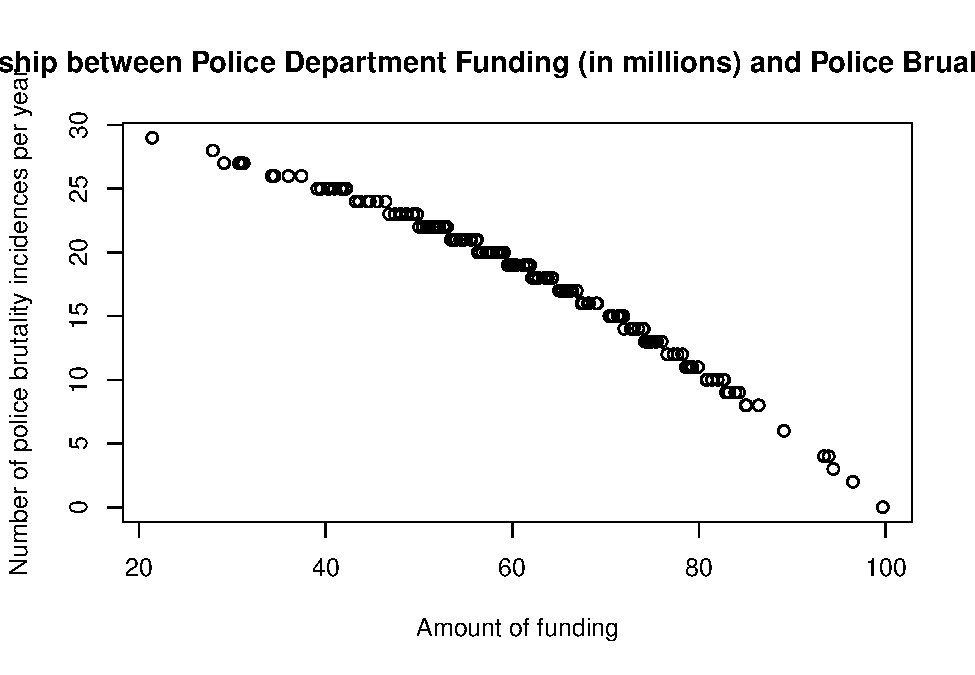
\includegraphics{Journal_files/figure-latex/unnamed-chunk-31-1.pdf}

\begin{Shaded}
\begin{Highlighting}[]
\FunctionTok{cor}\NormalTok{(dat}\SpecialCharTok{$}\NormalTok{funds, dat}\SpecialCharTok{$}\NormalTok{po.brut)}
\end{Highlighting}
\end{Shaded}

\begin{verbatim}
## [1] -0.9854706
\end{verbatim}

The dataset has three different variables consisting of the department
code, funds, and police brutality. There are 200 observations of
different police departments and the number of incidences where police
brutality occurred. We see that on average a department gets around 61
million dollars in funding and will have about 18 incidences of police
brutality that year. We can see from the graph that there is a clear
decrease in the number of police brutality incidences as the amount of
funding goes up. Furthermore, we can see that the correlation between
these two values is a -0.98 which indicates there is a extremely strong
linear relationship (in this case it is a negative one).

\hypertarget{problem-2-linear-regression-30-points}{%
\subsection{Problem 2: Linear regression (30
points)}\label{problem-2-linear-regression-30-points}}

\begin{enumerate}
\def\labelenumi{\alph{enumi}.}
\tightlist
\item
  Perform a simple linear regression to answer the question of interest.
  To do this, name your linear model ``reg.output'' and write the
  summary of the regression by using ``summary(reg.output)''.
\end{enumerate}

\begin{Shaded}
\begin{Highlighting}[]
\CommentTok{\# Remember to remove eval=FALSE!!}
\NormalTok{reg.output }\OtherTok{\textless{}{-}} \FunctionTok{lm}\NormalTok{(}\AttributeTok{formula =}\NormalTok{ dat}\SpecialCharTok{$}\NormalTok{po.brut }\SpecialCharTok{\textasciitilde{}}\NormalTok{ dat}\SpecialCharTok{$}\NormalTok{funds, }\AttributeTok{data =}\NormalTok{ dat)}
\FunctionTok{summary}\NormalTok{(reg.output)}
\end{Highlighting}
\end{Shaded}

\begin{verbatim}
## 
## Call:
## lm(formula = dat$po.brut ~ dat$funds, data = dat)
## 
## Residuals:
##     Min      1Q  Median      3Q     Max 
## -3.9433 -0.2233  0.2544  0.5952  1.1803 
## 
## Coefficients:
##              Estimate Std. Error t value Pr(>|t|)    
## (Intercept) 40.543069   0.282503  143.51   <2e-16 ***
## dat$funds   -0.367099   0.004496  -81.64   <2e-16 ***
## ---
## Signif. codes:  0 '***' 0.001 '**' 0.01 '*' 0.05 '.' 0.1 ' ' 1
## 
## Residual standard error: 0.9464 on 198 degrees of freedom
## Multiple R-squared:  0.9712, Adjusted R-squared:  0.971 
## F-statistic:  6666 on 1 and 198 DF,  p-value: < 2.2e-16
\end{verbatim}

\textbf{Your answer here.}

\begin{enumerate}
\def\labelenumi{\alph{enumi}.}
\setcounter{enumi}{1}
\tightlist
\item
  Report the estimated coefficient, standard error, and p-value of the
  slope. Is the relationship between funds and incidents statistically
  significant? Explain.
\end{enumerate}

The estimated coefficient for the slope is -0.367 while the estimated
coefficient for the intercept is 40.54. The p-value for the slope is
less than 2 x 10\^{}-16 (this is the same of the intercept as well).
These slope has a standard error of 0.0045 which means that regression
we have is very close to the actual value. This means that there exists
a linear relationship between the funds and the incidents statically as
each of these p-values are less than 0.05. This means that we can reject
the null hypothesis and assert that there is a linear relationship.

\begin{enumerate}
\def\labelenumi{\alph{enumi}.}
\setcounter{enumi}{2}
\tightlist
\item
  Draw a scatterplot of po.brut (y-axis) and funds (x-axis). Right below
  your plot command, use abline to draw the fitted regression line, like
  this:
\end{enumerate}

\begin{Shaded}
\begin{Highlighting}[]
\CommentTok{\# Remember to remove eval=FALSE!!}
\FunctionTok{plot}\NormalTok{(dat}\SpecialCharTok{$}\NormalTok{funds, dat}\SpecialCharTok{$}\NormalTok{po.brut,  }\AttributeTok{main=}\StringTok{"Relationship between Police Department Funding (in millions) and Police Bruality (per year)"}\NormalTok{, }\AttributeTok{xlab=}\StringTok{"Amount of funding"}\NormalTok{, }\AttributeTok{ylab=}\StringTok{"Number of police brutality incidences per year"}\NormalTok{)}
\FunctionTok{abline}\NormalTok{(reg.output, }\AttributeTok{col =} \StringTok{"red"}\NormalTok{, }\AttributeTok{lwd=}\DecValTok{2}\NormalTok{)}
\end{Highlighting}
\end{Shaded}

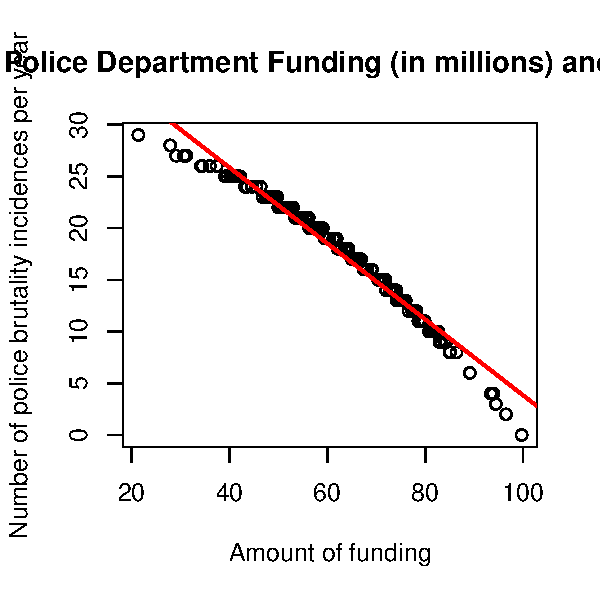
\includegraphics{Journal_files/figure-latex/unnamed-chunk-33-1.pdf} Does
the line look like a good fit? Why or why not?

For the middle values, the line follows the data precisely. However if
we look at the the tail-end of both sides of the data we can see that it
isn't as precise anymore. I believe that this line is an okay fit given
it can follow the distribution on average but when it gets to parts of
the data where we do not have as much information (the tail ends), the
predicted value isn't as correct.

\begin{enumerate}
\def\labelenumi{\alph{enumi}.}
\setcounter{enumi}{3}
\tightlist
\item
  Are the four assumptions of linear regression satisfied? To answer
  this, draw the relevant plots. (Write a maximum of one sentence per
  assumption.) If not, what might you try to do to improve this (if you
  had more time)?
\end{enumerate}

\begin{Shaded}
\begin{Highlighting}[]
\FunctionTok{plot}\NormalTok{(dat}\SpecialCharTok{$}\NormalTok{funds, reg.output}\SpecialCharTok{$}\NormalTok{residuals, }\AttributeTok{main=}\StringTok{"Residuals vs. x"}\NormalTok{, }\AttributeTok{xlab=}\StringTok{"x, Scaled speed"}\NormalTok{, }\AttributeTok{ylab=}\StringTok{"Residuals"}\NormalTok{)}
\FunctionTok{abline}\NormalTok{(}\AttributeTok{h =} \DecValTok{0}\NormalTok{, }\AttributeTok{lty=}\StringTok{"dashed"}\NormalTok{)}
\end{Highlighting}
\end{Shaded}

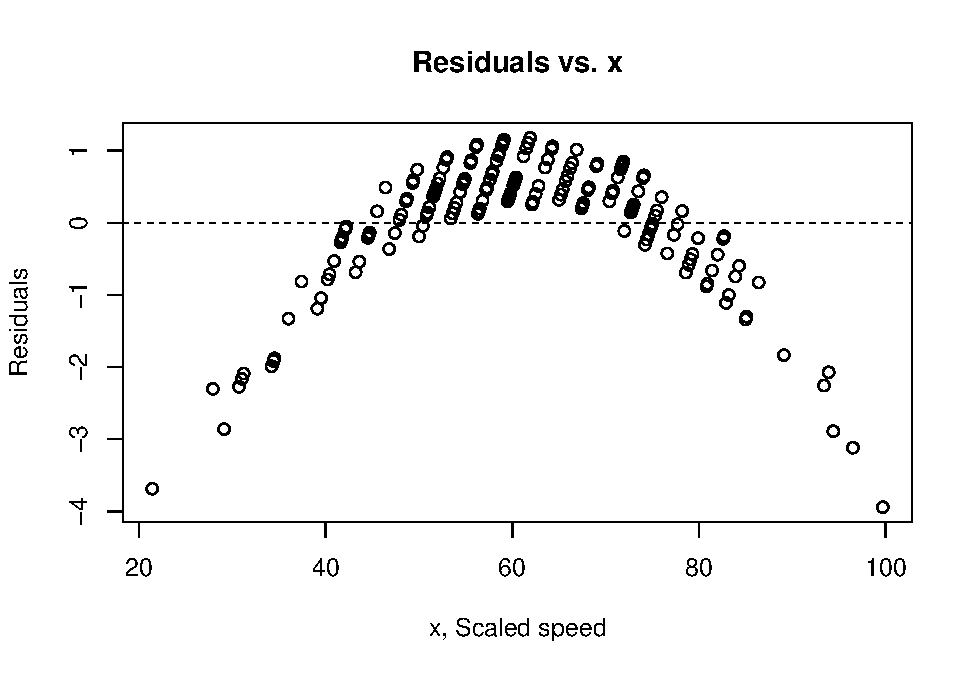
\includegraphics{Journal_files/figure-latex/unnamed-chunk-34-1.pdf}

\begin{Shaded}
\begin{Highlighting}[]
\FunctionTok{plot}\NormalTok{(reg.output, }\AttributeTok{which=}\DecValTok{1}\NormalTok{)}
\end{Highlighting}
\end{Shaded}

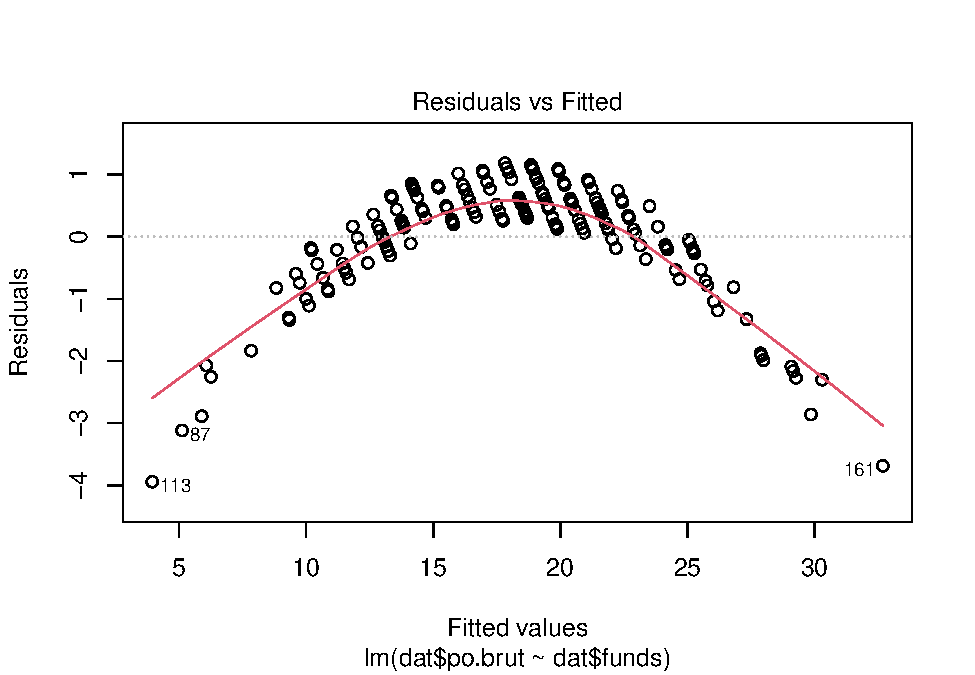
\includegraphics{Journal_files/figure-latex/unnamed-chunk-34-2.pdf}

\begin{Shaded}
\begin{Highlighting}[]
\FunctionTok{plot}\NormalTok{(dat}\SpecialCharTok{$}\NormalTok{funds, dat}\SpecialCharTok{$}\NormalTok{po.brut, }\AttributeTok{main=}\StringTok{"Relationship between funding and police brutality"}\NormalTok{, }\AttributeTok{xlab =} \StringTok{"Amount of funding"}\NormalTok{, }\AttributeTok{ylab =} \StringTok{"Number of police brutality incidences per year"}\NormalTok{)}
\end{Highlighting}
\end{Shaded}

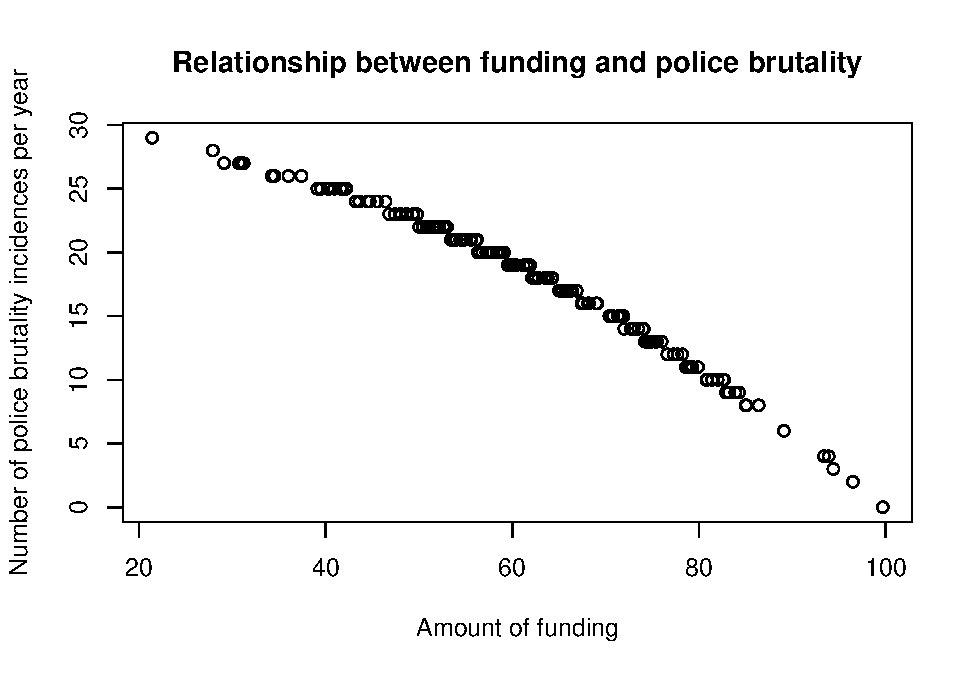
\includegraphics{Journal_files/figure-latex/unnamed-chunk-34-3.pdf}

\begin{Shaded}
\begin{Highlighting}[]
\FunctionTok{plot}\NormalTok{(reg.output, }\AttributeTok{which=}\DecValTok{3}\NormalTok{)}
\end{Highlighting}
\end{Shaded}

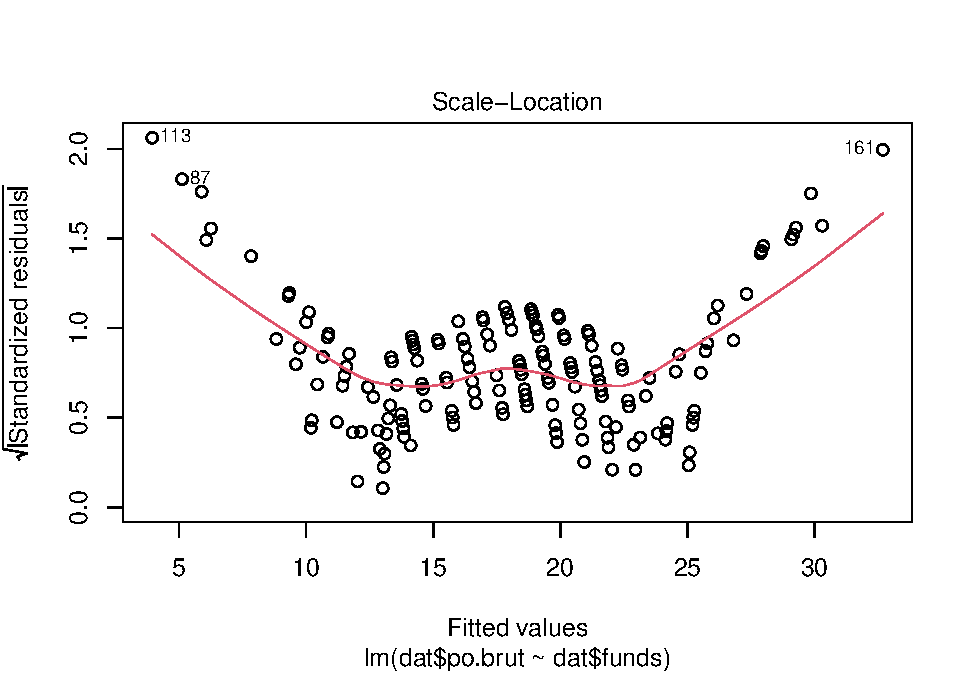
\includegraphics{Journal_files/figure-latex/unnamed-chunk-34-4.pdf}

\begin{Shaded}
\begin{Highlighting}[]
\FunctionTok{plot}\NormalTok{(reg.output, }\AttributeTok{which=}\DecValTok{5}\NormalTok{)}
\end{Highlighting}
\end{Shaded}

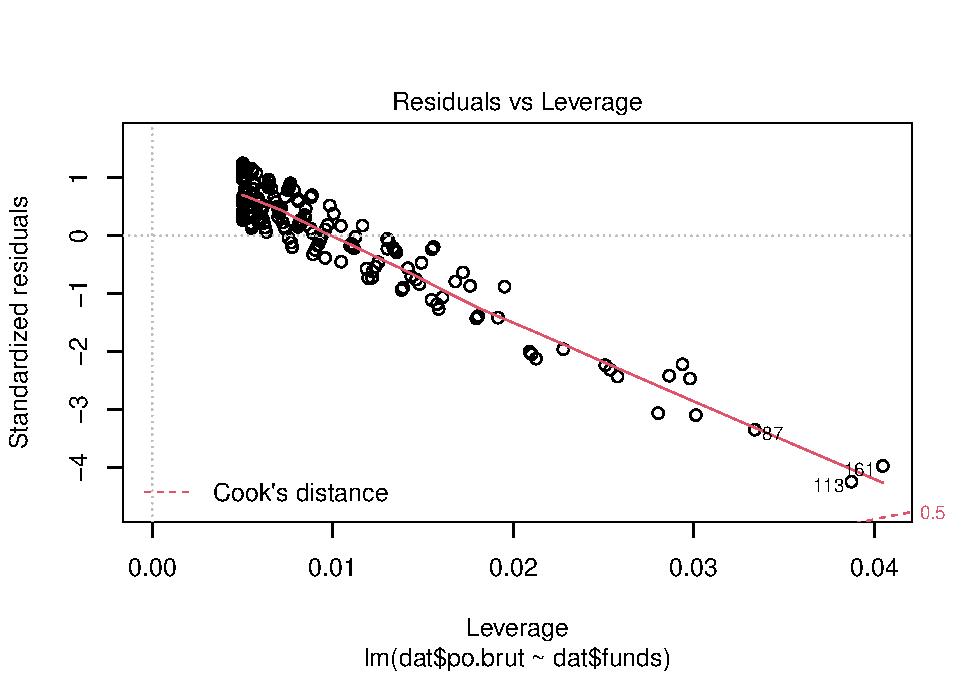
\includegraphics{Journal_files/figure-latex/unnamed-chunk-34-5.pdf}

\begin{Shaded}
\begin{Highlighting}[]
\FunctionTok{plot}\NormalTok{(reg.output, }\AttributeTok{which=}\DecValTok{2}\NormalTok{)}
\end{Highlighting}
\end{Shaded}

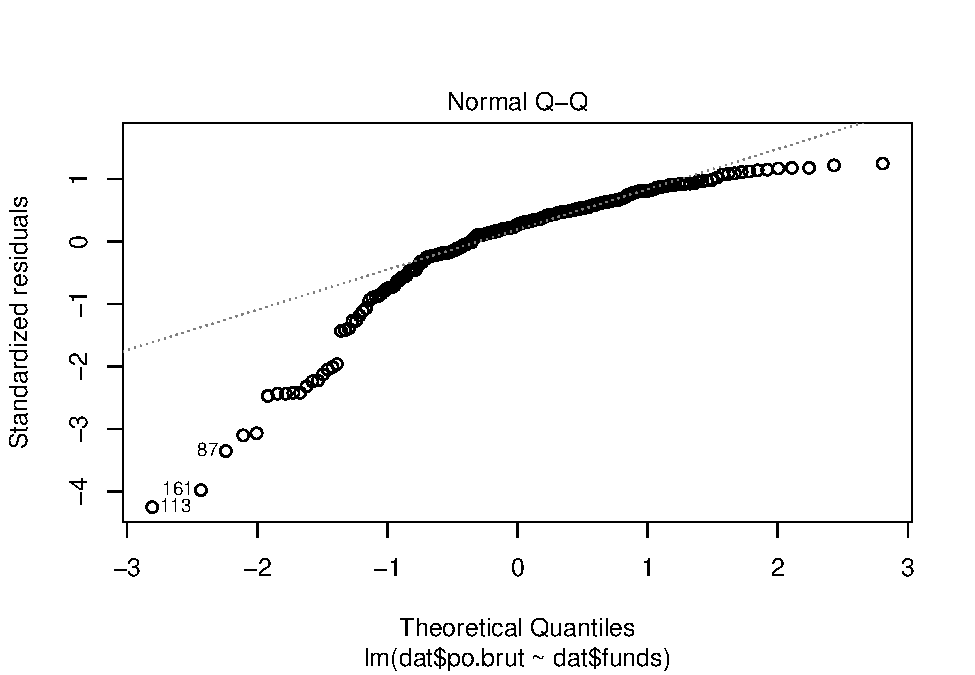
\includegraphics{Journal_files/figure-latex/unnamed-chunk-34-6.pdf}

1.Linearly Assumption: This assumption doesn't hold because we can
clearly see that the red line for the graph on residuals vs fitted is
not flat and the residuals vs x has a pattern, therefore this means
there is non constant variance.

2.Independence assumption : This doesn't hold because there is a pattern
in our graph for residuals vs x.

3.Equal variance assumption : This assumption probably doesn't hold
because our scale-location plot isn't straight and there is a pattern
with it.

4.Normal Population Assumption : When we look at our normal qq plot, we
see that the there is a left skew (the left and the right ends of the
tail are lighter and smaller than the normal distribution).

The four assumptions were not satisfied, next time I would try and get
more data or I could try and use a different model that would help us
see a better relationship, if there exists one.

\begin{enumerate}
\def\labelenumi{\alph{enumi}.}
\setcounter{enumi}{4}
\tightlist
\item
  Answer the question of interest based on your analysis.
\end{enumerate}

Because our assumptions do not hold, we can't use this linear regression
model to determine if more funding will lead to a decrease of police
brutality. This means the results that we obtained to reject the null
hypothesis can not be used and it is inconclusive. The results we
obtained are misleading.

\hypertarget{problem-3-data-ethics-10-points}{%
\subsection{Problem 3: Data ethics (10
points)}\label{problem-3-data-ethics-10-points}}

Describe the dataset. Considering our lecture on data ethics, what
concerns do you have about the dataset? Once you perform your analysis
to answer the question of interest using this dataset, what concerns
might you have about the results?

This dataset gives us the funding a police department receives and the
amount of police brutality that occurs. From our data ethics lecture, an
issue we could come across is correlation doesn't imply causation. So
even though we have a very high correlation, this doesn't necessary mean
that the two variables are related. People could potentially look at
this correlation and see the regression without realizing that our
assumption didn't hold.

This matters because people could use this data or data like this to
push a false narrative that could damage people. This is an important
example to see that we have to check everything because if we forget and
show some false information it could cause people to believe ideas that
are not true.

\hypertarget{assignment-4}{%
\section{Assignment 4}\label{assignment-4}}

\hypertarget{data-visualization-active-reading}{%
\subsection{Data Visualization -- Active
Reading}\label{data-visualization-active-reading}}

\begin{enumerate}
\def\labelenumi{\arabic{enumi}.}
\tightlist
\item
  Installed tidyverse and imported it.
\end{enumerate}

\begin{Shaded}
\begin{Highlighting}[]
\FunctionTok{library}\NormalTok{(tidyverse)}
\FunctionTok{library}\NormalTok{(ggplot2)}
\end{Highlighting}
\end{Shaded}

\begin{enumerate}
\def\labelenumi{\arabic{enumi}.}
\setcounter{enumi}{1}
\tightlist
\item
  run mpg dataframe
\end{enumerate}

\begin{Shaded}
\begin{Highlighting}[]
\NormalTok{mpg}
\end{Highlighting}
\end{Shaded}

\begin{verbatim}
## # A tibble: 234 x 11
##    manufacturer model      displ  year   cyl trans drv     cty   hwy fl    class
##    <chr>        <chr>      <dbl> <int> <int> <chr> <chr> <int> <int> <chr> <chr>
##  1 audi         a4           1.8  1999     4 auto~ f        18    29 p     comp~
##  2 audi         a4           1.8  1999     4 manu~ f        21    29 p     comp~
##  3 audi         a4           2    2008     4 manu~ f        20    31 p     comp~
##  4 audi         a4           2    2008     4 auto~ f        21    30 p     comp~
##  5 audi         a4           2.8  1999     6 auto~ f        16    26 p     comp~
##  6 audi         a4           2.8  1999     6 manu~ f        18    26 p     comp~
##  7 audi         a4           3.1  2008     6 auto~ f        18    27 p     comp~
##  8 audi         a4 quattro   1.8  1999     4 manu~ 4        18    26 p     comp~
##  9 audi         a4 quattro   1.8  1999     4 auto~ 4        16    25 p     comp~
## 10 audi         a4 quattro   2    2008     4 manu~ 4        20    28 p     comp~
## # ... with 224 more rows
\end{verbatim}

displ, a car's engine size, in litres.

hwy, a car's fuel efficiency on the highway, in miles per gallon (mpg).
A car with a low fuel efficiency consumes more fuel than a car with a
high fuel efficiency when they travel the same distanc

\begin{enumerate}
\def\labelenumi{\arabic{enumi}.}
\setcounter{enumi}{2}
\tightlist
\item
  Creating a ggplot
\end{enumerate}

\begin{Shaded}
\begin{Highlighting}[]
\FunctionTok{ggplot}\NormalTok{(}\AttributeTok{data =}\NormalTok{ mpg) }\SpecialCharTok{+} 
  \FunctionTok{geom\_point}\NormalTok{(}\AttributeTok{mapping =} \FunctionTok{aes}\NormalTok{(}\AttributeTok{x =}\NormalTok{ displ, }\AttributeTok{y =}\NormalTok{ hwy))}
\end{Highlighting}
\end{Shaded}

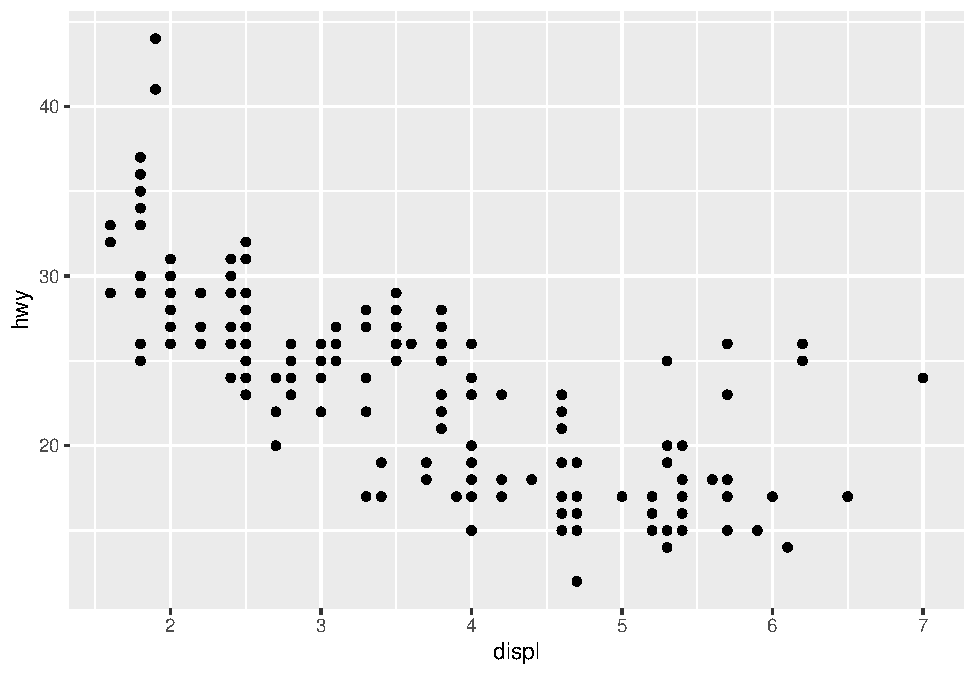
\includegraphics{Journal_files/figure-latex/unnamed-chunk-37-1.pdf}

The plot shows a negative relationship between engine size (displ) and
fuel efficiency (hwy). In other words, cars with big engines use more
fuel. Does this confirm or refute your hypothesis about fuel efficiency
and engine size?

With ggplot2, you begin a plot with the function ggplot(). ggplot()
creates a coordinate system that you can add layers to. The first
argument of ggplot() is the dataset to use in the graph. So ggplot(data
= mpg) creates an empty graph, but it's not very interesting so I'm not
going to show it here.

You complete your graph by adding one or more layers to ggplot(). The
function geom\_point() adds a layer of points to your plot, which
creates a scatterplot. ggplot2 comes with many geom functions that each
add a different type of layer to a plot. You'll learn a whole bunch of
them throughout this chapter.

Each geom function in ggplot2 takes a mapping argument. This defines how
variables in your dataset are mapped to visual properties. The mapping
argument is always paired with aes(), and the x and y arguments of aes()
specify which variables to map to the x and y axes. ggplot2 looks for
the mapped variables in the data argument, in this case, mpg.

This can be represented in the following template.

ggplot(data = ) + (mapping = aes())

\begin{Shaded}
\begin{Highlighting}[]
\FunctionTok{dim}\NormalTok{(mpg)}
\end{Highlighting}
\end{Shaded}

\begin{verbatim}
## [1] 234  11
\end{verbatim}

\begin{Shaded}
\begin{Highlighting}[]
\NormalTok{?mpg}

\FunctionTok{plot}\NormalTok{(mpg}\SpecialCharTok{$}\NormalTok{hwy, mpg}\SpecialCharTok{$}\NormalTok{cyl)}
\end{Highlighting}
\end{Shaded}

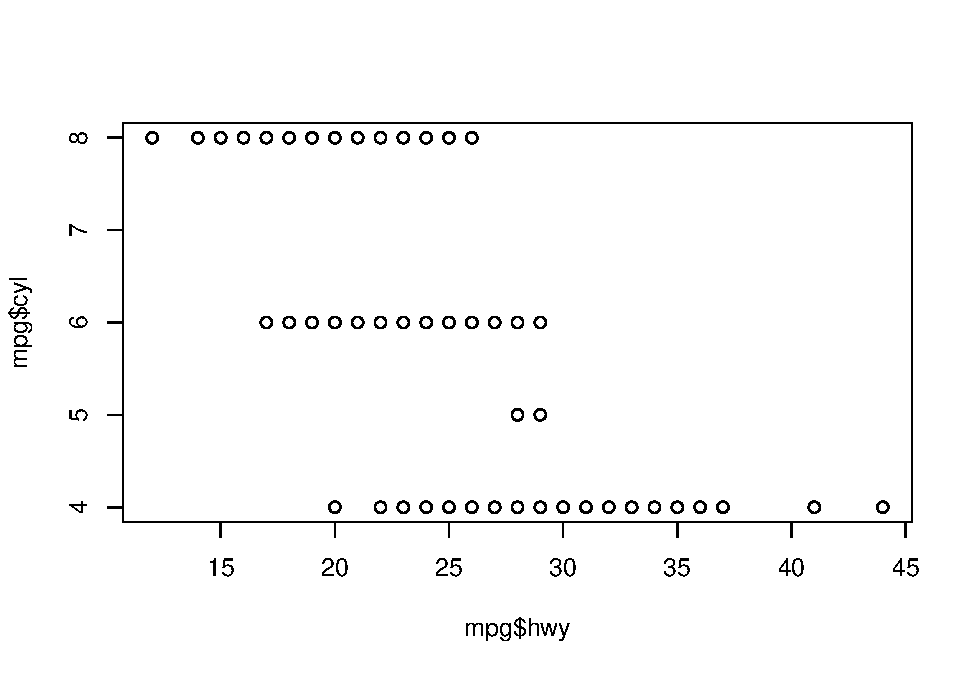
\includegraphics{Journal_files/figure-latex/unnamed-chunk-38-1.pdf} 1. I
see nothing 2. There are 234 rows and 11 columns 3. drv is the type of
drive train where f = front-wheel drive, r = rear wheel drive, 4 = 4wd
4. Its not useful because it is numerical

\begin{enumerate}
\def\labelenumi{\arabic{enumi}.}
\setcounter{enumi}{3}
\tightlist
\item
\end{enumerate}

\begin{Shaded}
\begin{Highlighting}[]
\FunctionTok{ggplot}\NormalTok{(}\AttributeTok{data =}\NormalTok{ mpg) }\SpecialCharTok{+} 
  \FunctionTok{geom\_point}\NormalTok{(}\AttributeTok{mapping =} \FunctionTok{aes}\NormalTok{(}\AttributeTok{x =}\NormalTok{ displ, }\AttributeTok{y =}\NormalTok{ hwy, }\AttributeTok{color =}\NormalTok{ class))}
\end{Highlighting}
\end{Shaded}

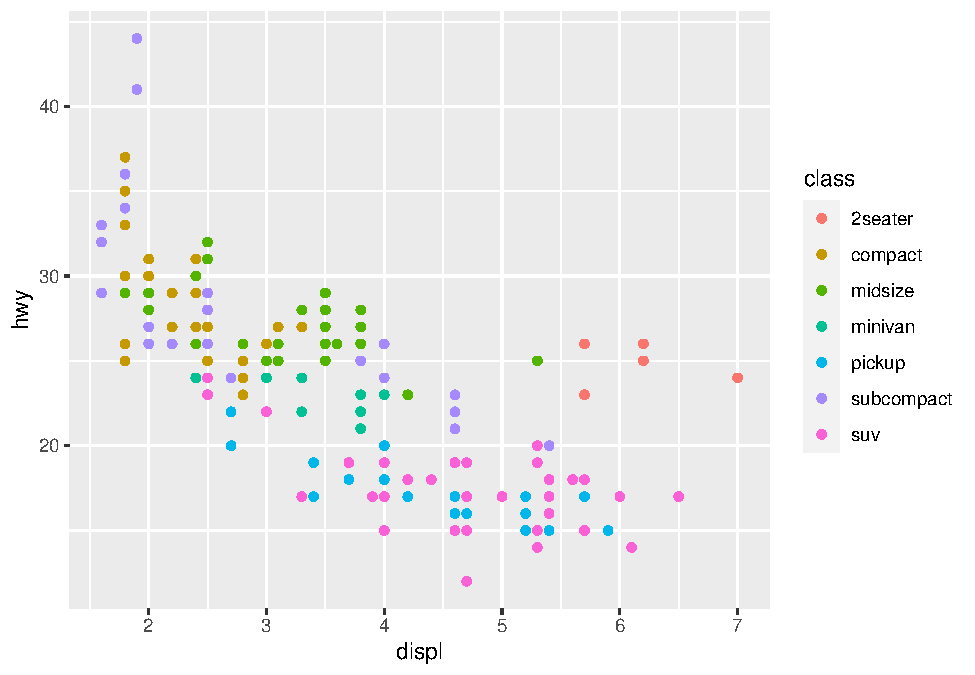
\includegraphics{Journal_files/figure-latex/unnamed-chunk-39-1.pdf}

\begin{Shaded}
\begin{Highlighting}[]
\FunctionTok{ggplot}\NormalTok{(}\AttributeTok{data =}\NormalTok{ mpg) }\SpecialCharTok{+} 
  \FunctionTok{geom\_point}\NormalTok{(}\AttributeTok{mapping =} \FunctionTok{aes}\NormalTok{(}\AttributeTok{x =}\NormalTok{ displ, }\AttributeTok{y =}\NormalTok{ hwy, }\AttributeTok{size =}\NormalTok{ class))}
\end{Highlighting}
\end{Shaded}

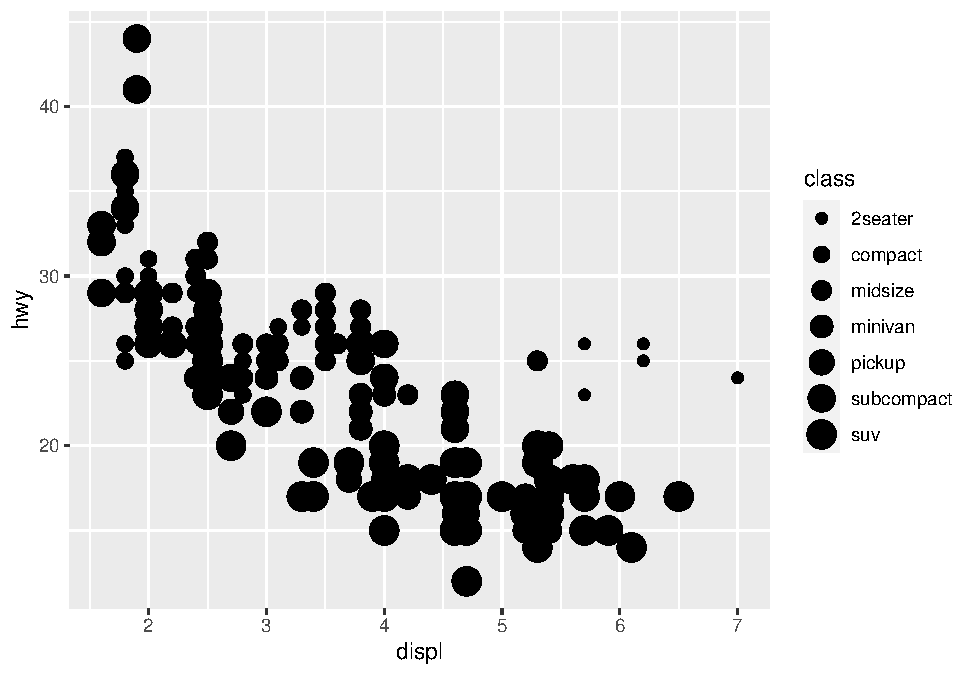
\includegraphics{Journal_files/figure-latex/unnamed-chunk-39-2.pdf}

\begin{Shaded}
\begin{Highlighting}[]
\CommentTok{\#\textgreater{} Warning: Using size for a discrete variable is not advised.}

\CommentTok{\# Left}
\FunctionTok{ggplot}\NormalTok{(}\AttributeTok{data =}\NormalTok{ mpg) }\SpecialCharTok{+} 
  \FunctionTok{geom\_point}\NormalTok{(}\AttributeTok{mapping =} \FunctionTok{aes}\NormalTok{(}\AttributeTok{x =}\NormalTok{ displ, }\AttributeTok{y =}\NormalTok{ hwy, }\AttributeTok{alpha =}\NormalTok{ class))}
\end{Highlighting}
\end{Shaded}

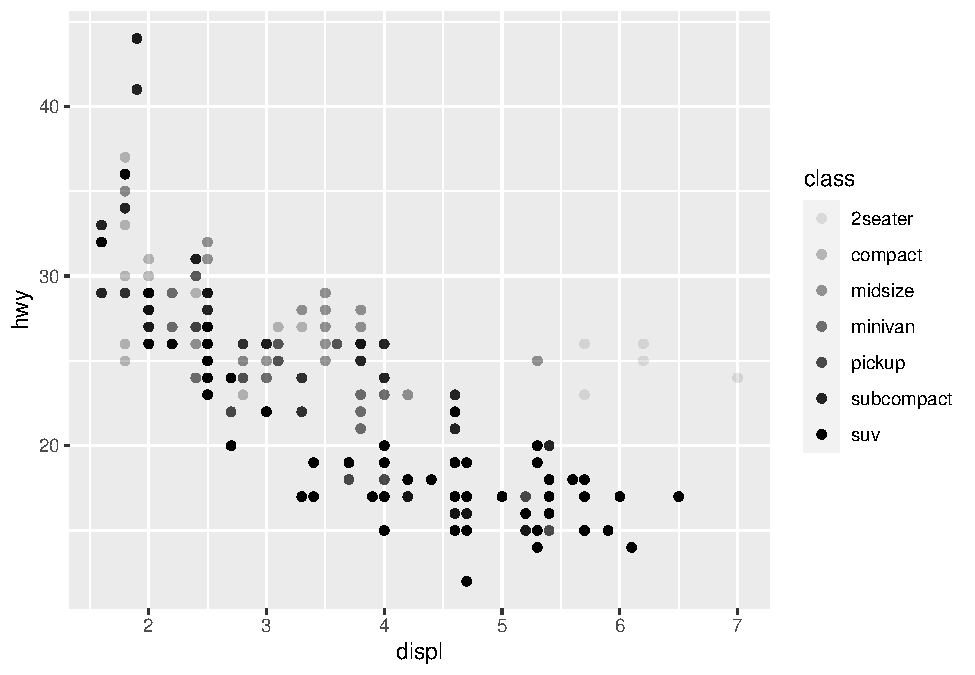
\includegraphics{Journal_files/figure-latex/unnamed-chunk-39-3.pdf}

\begin{Shaded}
\begin{Highlighting}[]
\CommentTok{\# Right}
\FunctionTok{ggplot}\NormalTok{(}\AttributeTok{data =}\NormalTok{ mpg) }\SpecialCharTok{+} 
  \FunctionTok{geom\_point}\NormalTok{(}\AttributeTok{mapping =} \FunctionTok{aes}\NormalTok{(}\AttributeTok{x =}\NormalTok{ displ, }\AttributeTok{y =}\NormalTok{ hwy, }\AttributeTok{shape =}\NormalTok{ class))}
\end{Highlighting}
\end{Shaded}

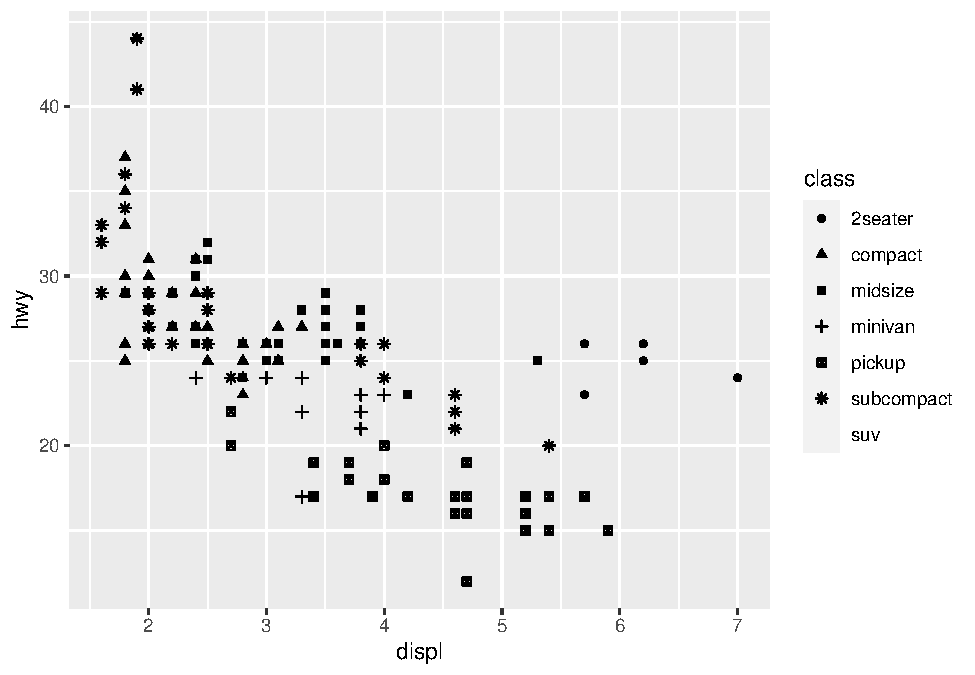
\includegraphics{Journal_files/figure-latex/unnamed-chunk-39-4.pdf}

\begin{Shaded}
\begin{Highlighting}[]
\FunctionTok{ggplot}\NormalTok{(}\AttributeTok{data =}\NormalTok{ mpg) }\SpecialCharTok{+} 
  \FunctionTok{geom\_point}\NormalTok{(}\AttributeTok{mapping =} \FunctionTok{aes}\NormalTok{(}\AttributeTok{x =}\NormalTok{ displ, }\AttributeTok{y =}\NormalTok{ hwy), }\AttributeTok{color =} \StringTok{"blue"}\NormalTok{)}
\end{Highlighting}
\end{Shaded}

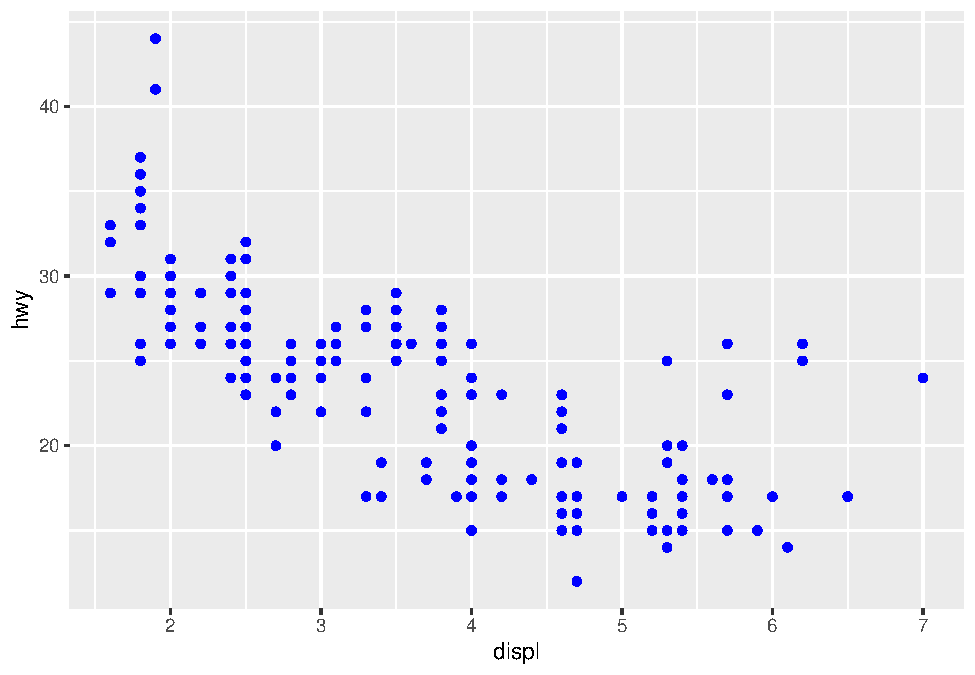
\includegraphics{Journal_files/figure-latex/unnamed-chunk-39-5.pdf} We
can use aes to change how our plots look. This refers to aesthetics and
ggplot will change it for us.

shape changes shape (only does 6 groups). alpha changes transparency.
color changes color

You can also change the color manually.

Common problems are that people will put the + in the wrong place like
here: ggplot(data = mpg) + geom\_point(mapping = aes(x = displ, y =
hwy))

\begin{Shaded}
\begin{Highlighting}[]
\FunctionTok{ggplot}\NormalTok{(}\AttributeTok{data =}\NormalTok{ mpg) }\SpecialCharTok{+} 
  \FunctionTok{geom\_point}\NormalTok{(}\AttributeTok{mapping =} \FunctionTok{aes}\NormalTok{(}\AttributeTok{x =}\NormalTok{ displ, }\AttributeTok{y =}\NormalTok{ hwy)) }\SpecialCharTok{+} 
  \FunctionTok{facet\_wrap}\NormalTok{(}\SpecialCharTok{\textasciitilde{}}\NormalTok{ class, }\AttributeTok{nrow =} \DecValTok{2}\NormalTok{)}
\end{Highlighting}
\end{Shaded}

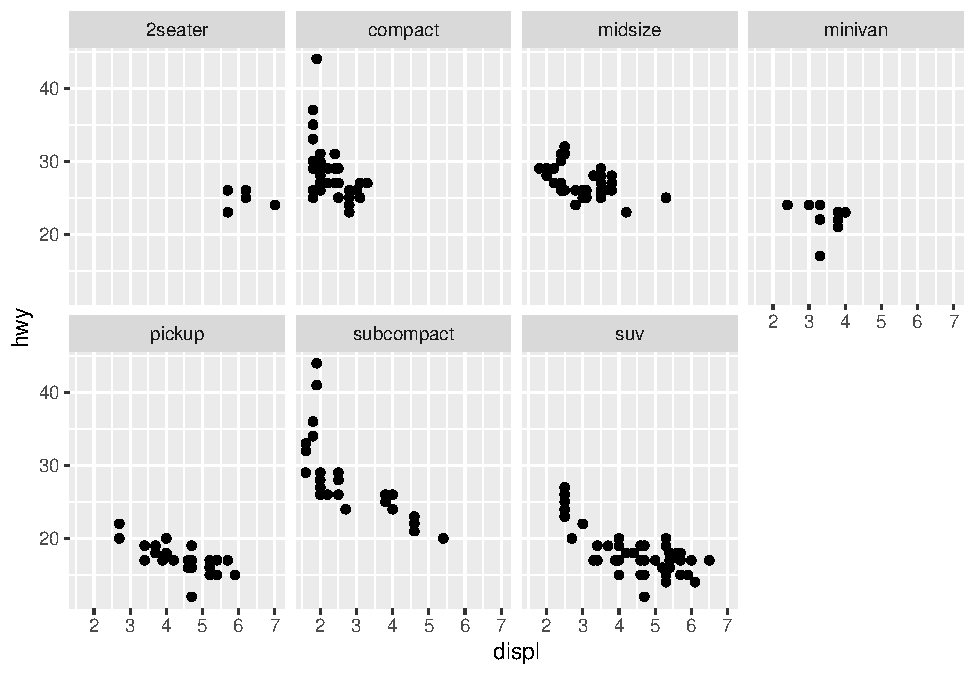
\includegraphics{Journal_files/figure-latex/unnamed-chunk-40-1.pdf}

\begin{Shaded}
\begin{Highlighting}[]
\FunctionTok{ggplot}\NormalTok{(}\AttributeTok{data =}\NormalTok{ mpg) }\SpecialCharTok{+} 
  \FunctionTok{geom\_point}\NormalTok{(}\AttributeTok{mapping =} \FunctionTok{aes}\NormalTok{(}\AttributeTok{x =}\NormalTok{ displ, }\AttributeTok{y =}\NormalTok{ hwy)) }\SpecialCharTok{+} 
  \FunctionTok{facet\_grid}\NormalTok{(drv }\SpecialCharTok{\textasciitilde{}}\NormalTok{ cyl)}
\end{Highlighting}
\end{Shaded}

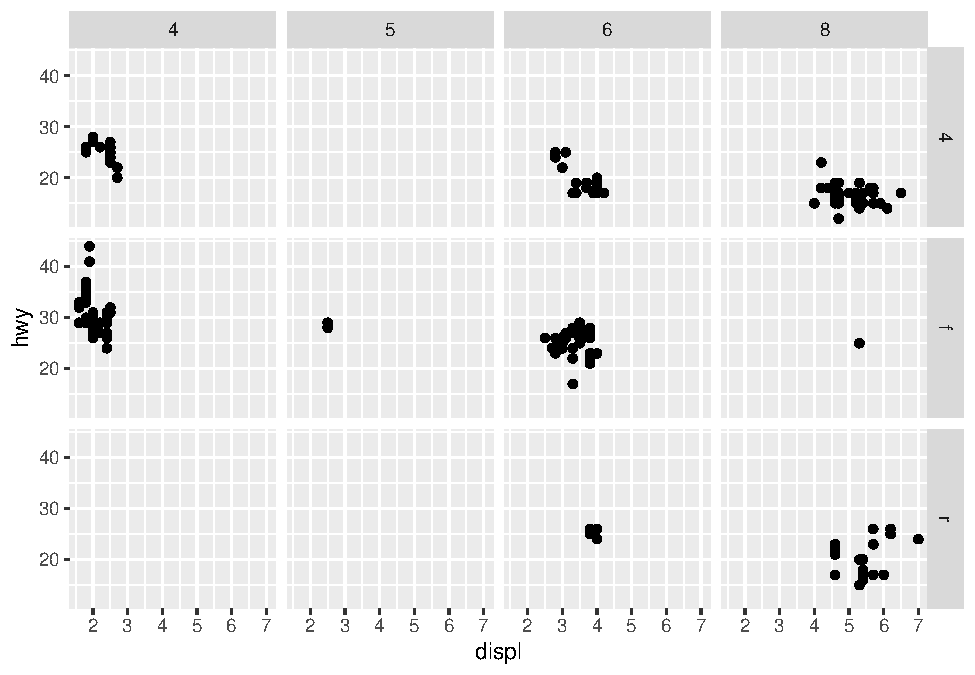
\includegraphics{Journal_files/figure-latex/unnamed-chunk-40-2.pdf}

One way to add additional variables is with aesthetics. Another way,
particularly useful for categorical variables, is to split your plot
into facets, subplots that each display one subset of the data.

To facet your plot by a single variable, use facet\_wrap(). The first
argument of facet\_wrap() should be a formula, which you create with
\textasciitilde{} followed by a variable name (here ``formula'' is the
name of a data structure in R, not a synonym for ``equation''). The
variable that you pass to facet\_wrap() should be discrete.

We can add a combination of two variable by using facet\_grid.

\begin{Shaded}
\begin{Highlighting}[]
\CommentTok{\# left}
\FunctionTok{ggplot}\NormalTok{(}\AttributeTok{data =}\NormalTok{ mpg) }\SpecialCharTok{+} 
  \FunctionTok{geom\_point}\NormalTok{(}\AttributeTok{mapping =} \FunctionTok{aes}\NormalTok{(}\AttributeTok{x =}\NormalTok{ displ, }\AttributeTok{y =}\NormalTok{ hwy))}
\end{Highlighting}
\end{Shaded}

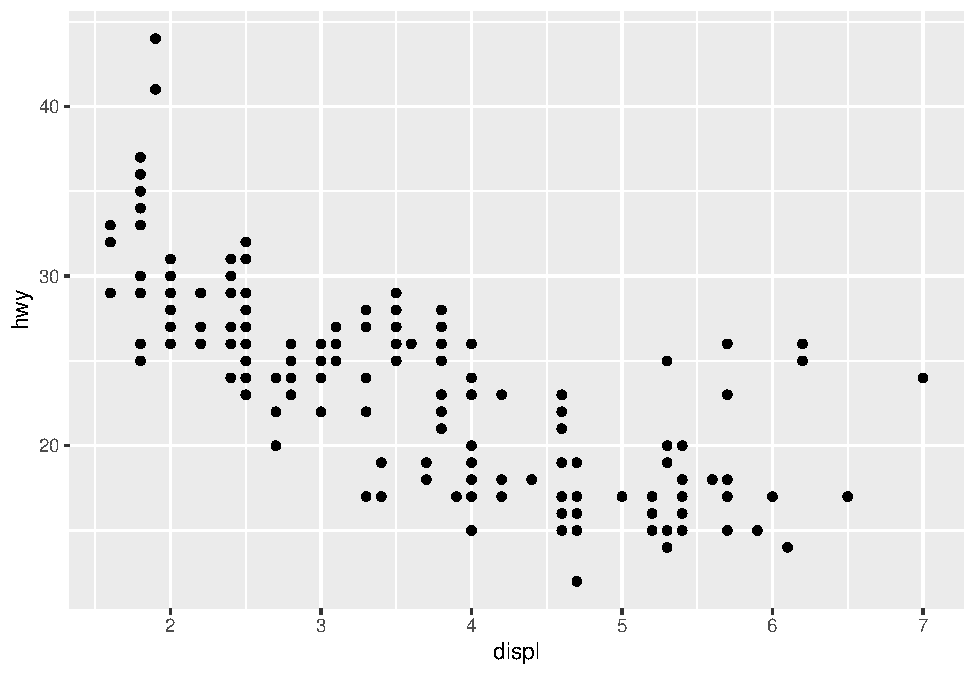
\includegraphics{Journal_files/figure-latex/unnamed-chunk-41-1.pdf}

\begin{Shaded}
\begin{Highlighting}[]
\CommentTok{\# right}
\FunctionTok{ggplot}\NormalTok{(}\AttributeTok{data =}\NormalTok{ mpg) }\SpecialCharTok{+} 
  \FunctionTok{geom\_smooth}\NormalTok{(}\AttributeTok{mapping =} \FunctionTok{aes}\NormalTok{(}\AttributeTok{x =}\NormalTok{ displ, }\AttributeTok{y =}\NormalTok{ hwy))}
\end{Highlighting}
\end{Shaded}

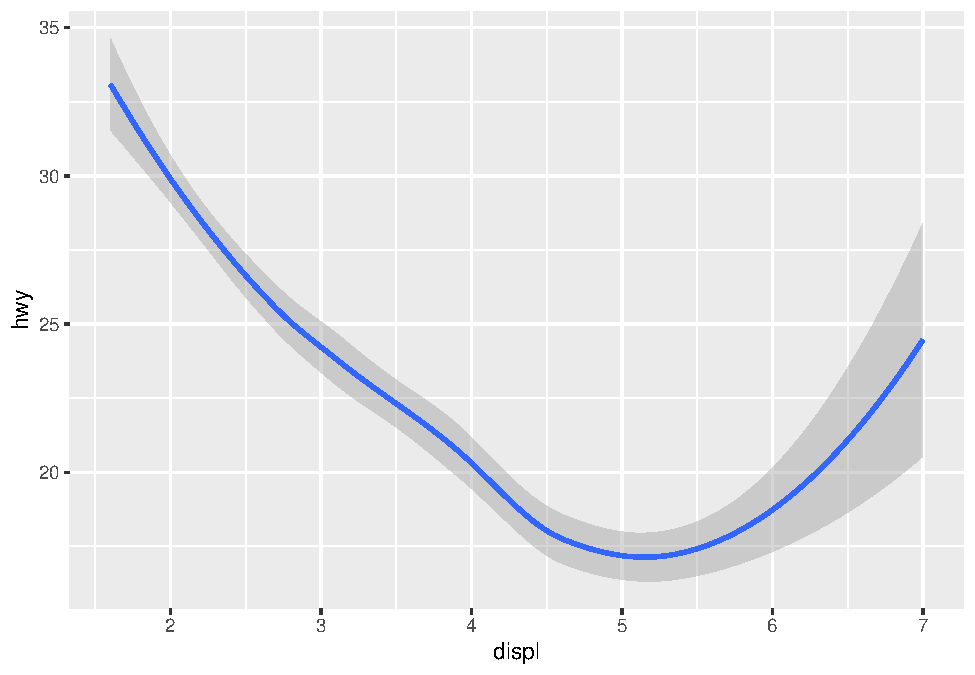
\includegraphics{Journal_files/figure-latex/unnamed-chunk-41-2.pdf}

\begin{Shaded}
\begin{Highlighting}[]
\FunctionTok{ggplot}\NormalTok{(}\AttributeTok{data =}\NormalTok{ mpg) }\SpecialCharTok{+} 
  \FunctionTok{geom\_smooth}\NormalTok{(}\AttributeTok{mapping =} \FunctionTok{aes}\NormalTok{(}\AttributeTok{x =}\NormalTok{ displ, }\AttributeTok{y =}\NormalTok{ hwy, }\AttributeTok{linetype =}\NormalTok{ drv))}
\end{Highlighting}
\end{Shaded}

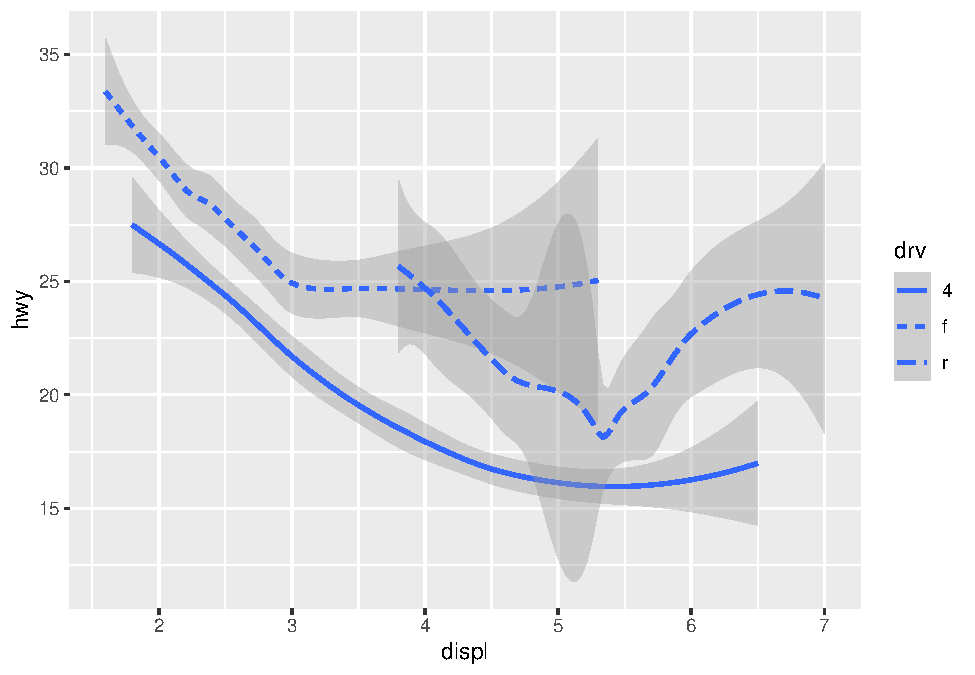
\includegraphics{Journal_files/figure-latex/unnamed-chunk-41-3.pdf} We
can also work with geometric objects in our plot to help with
visualization. Additionally we can also change the linetype so it is
different for each unique value.

ggplot provides over 40 geom plots that we can use to help with data
visualization

\begin{Shaded}
\begin{Highlighting}[]
\FunctionTok{ggplot}\NormalTok{(}\AttributeTok{data =}\NormalTok{ mpg) }\SpecialCharTok{+}
  \FunctionTok{geom\_smooth}\NormalTok{(}\AttributeTok{mapping =} \FunctionTok{aes}\NormalTok{(}\AttributeTok{x =}\NormalTok{ displ, }\AttributeTok{y =}\NormalTok{ hwy))}
\end{Highlighting}
\end{Shaded}

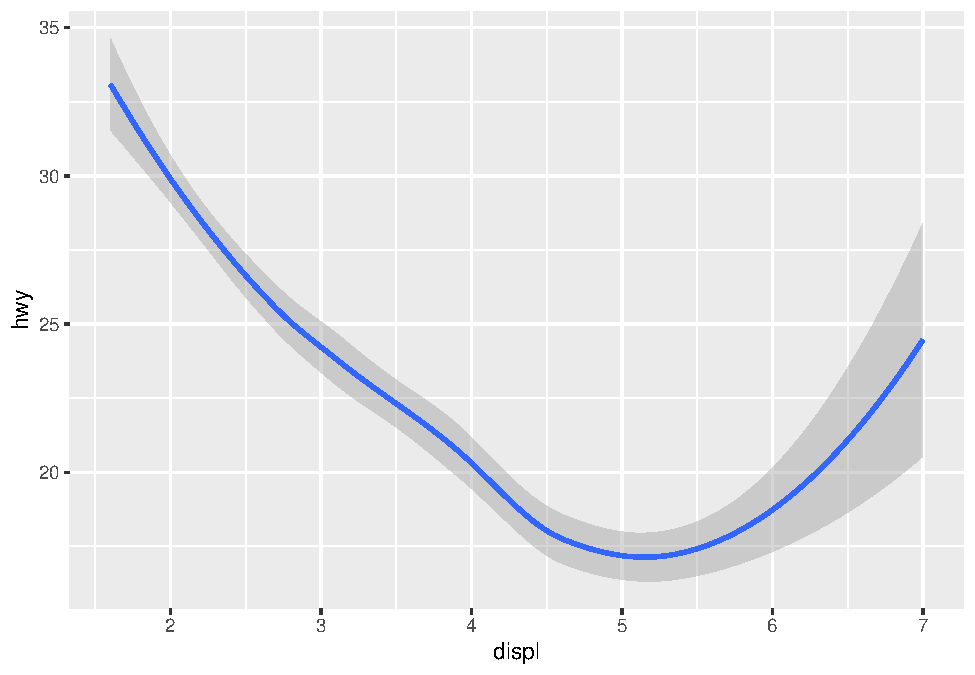
\includegraphics{Journal_files/figure-latex/unnamed-chunk-42-1.pdf}

\begin{Shaded}
\begin{Highlighting}[]
\FunctionTok{ggplot}\NormalTok{(}\AttributeTok{data =}\NormalTok{ mpg) }\SpecialCharTok{+}
  \FunctionTok{geom\_smooth}\NormalTok{(}\AttributeTok{mapping =} \FunctionTok{aes}\NormalTok{(}\AttributeTok{x =}\NormalTok{ displ, }\AttributeTok{y =}\NormalTok{ hwy, }\AttributeTok{group =}\NormalTok{ drv))}
\end{Highlighting}
\end{Shaded}

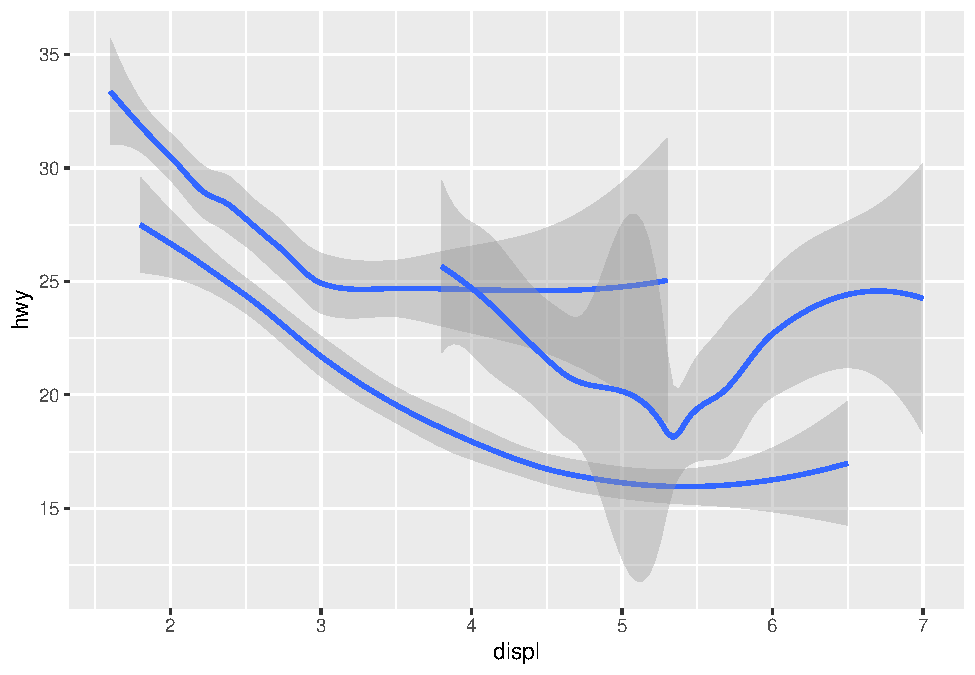
\includegraphics{Journal_files/figure-latex/unnamed-chunk-42-2.pdf}

\begin{Shaded}
\begin{Highlighting}[]
\FunctionTok{ggplot}\NormalTok{(}\AttributeTok{data =}\NormalTok{ mpg) }\SpecialCharTok{+}
  \FunctionTok{geom\_smooth}\NormalTok{(}
    \AttributeTok{mapping =} \FunctionTok{aes}\NormalTok{(}\AttributeTok{x =}\NormalTok{ displ, }\AttributeTok{y =}\NormalTok{ hwy, }\AttributeTok{color =}\NormalTok{ drv),}
    \AttributeTok{show.legend =} \ConstantTok{FALSE}
\NormalTok{  )}
\end{Highlighting}
\end{Shaded}

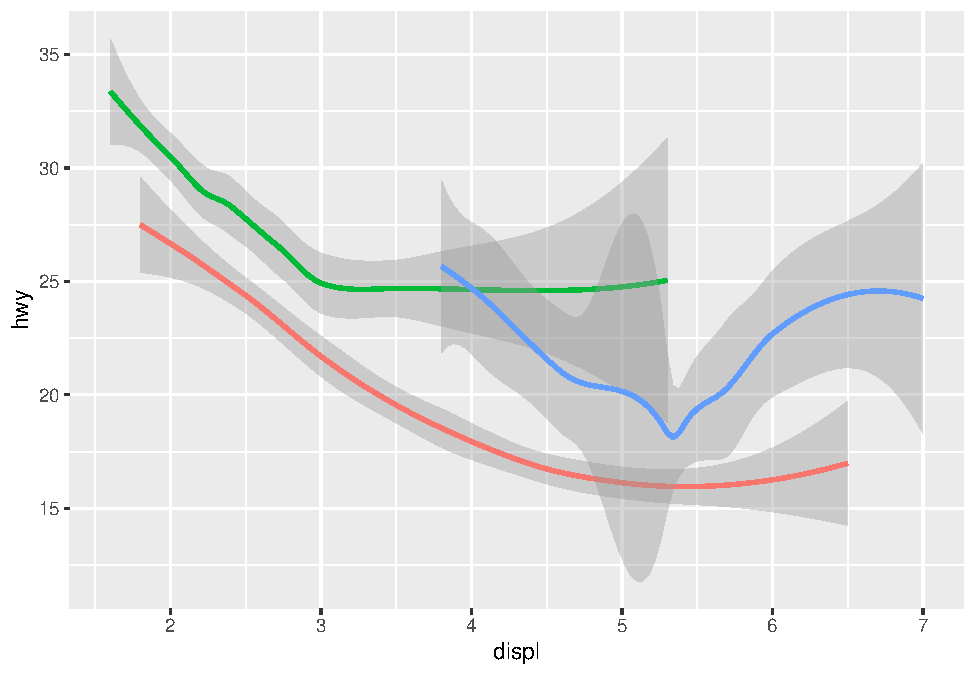
\includegraphics{Journal_files/figure-latex/unnamed-chunk-42-3.pdf} We
can also display multiple geom on a single plot.

\begin{Shaded}
\begin{Highlighting}[]
\FunctionTok{ggplot}\NormalTok{(}\AttributeTok{data =}\NormalTok{ mpg) }\SpecialCharTok{+} 
  \FunctionTok{geom\_point}\NormalTok{(}\AttributeTok{mapping =} \FunctionTok{aes}\NormalTok{(}\AttributeTok{x =}\NormalTok{ displ, }\AttributeTok{y =}\NormalTok{ hwy)) }\SpecialCharTok{+}
  \FunctionTok{geom\_smooth}\NormalTok{(}\AttributeTok{mapping =} \FunctionTok{aes}\NormalTok{(}\AttributeTok{x =}\NormalTok{ displ, }\AttributeTok{y =}\NormalTok{ hwy))}
\end{Highlighting}
\end{Shaded}

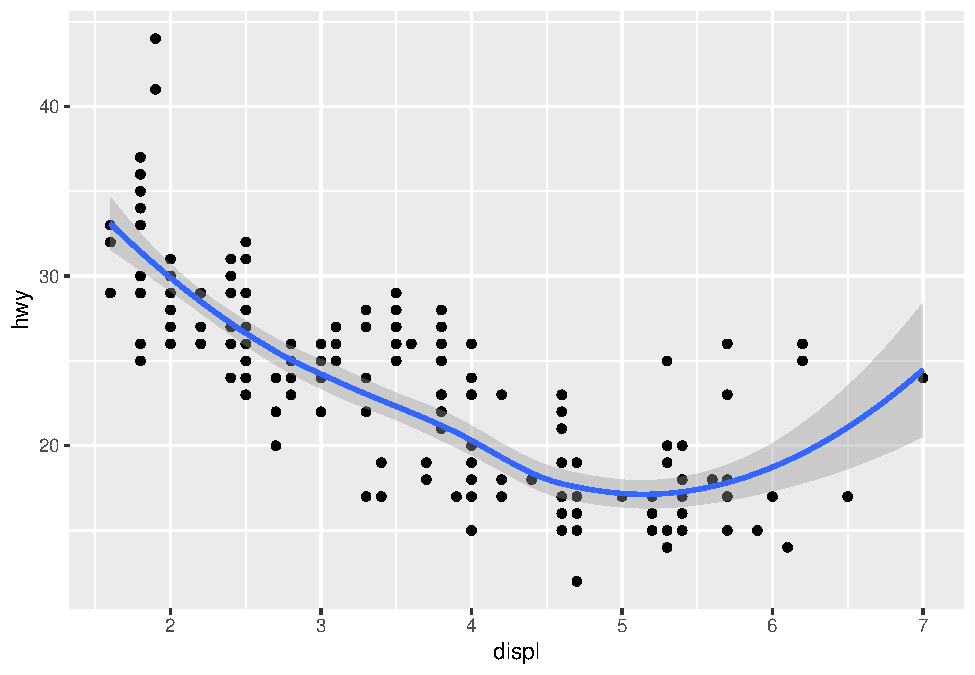
\includegraphics{Journal_files/figure-latex/unnamed-chunk-43-1.pdf}

\begin{Shaded}
\begin{Highlighting}[]
\FunctionTok{ggplot}\NormalTok{(}\AttributeTok{data =}\NormalTok{ mpg, }\AttributeTok{mapping =} \FunctionTok{aes}\NormalTok{(}\AttributeTok{x =}\NormalTok{ displ, }\AttributeTok{y =}\NormalTok{ hwy)) }\SpecialCharTok{+} 
  \FunctionTok{geom\_point}\NormalTok{() }\SpecialCharTok{+} 
  \FunctionTok{geom\_smooth}\NormalTok{()}
\end{Highlighting}
\end{Shaded}

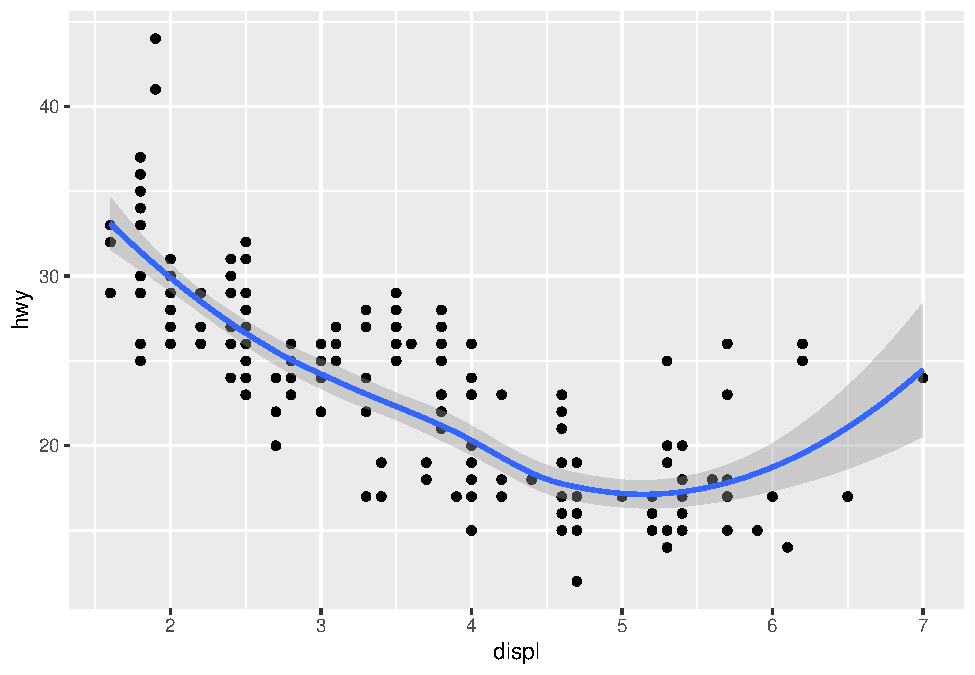
\includegraphics{Journal_files/figure-latex/unnamed-chunk-43-2.pdf}

\begin{Shaded}
\begin{Highlighting}[]
\FunctionTok{ggplot}\NormalTok{(}\AttributeTok{data =}\NormalTok{ mpg, }\AttributeTok{mapping =} \FunctionTok{aes}\NormalTok{(}\AttributeTok{x =}\NormalTok{ displ, }\AttributeTok{y =}\NormalTok{ hwy)) }\SpecialCharTok{+} 
  \FunctionTok{geom\_point}\NormalTok{(}\AttributeTok{mapping =} \FunctionTok{aes}\NormalTok{(}\AttributeTok{color =}\NormalTok{ class)) }\SpecialCharTok{+} 
  \FunctionTok{geom\_smooth}\NormalTok{()}
\end{Highlighting}
\end{Shaded}

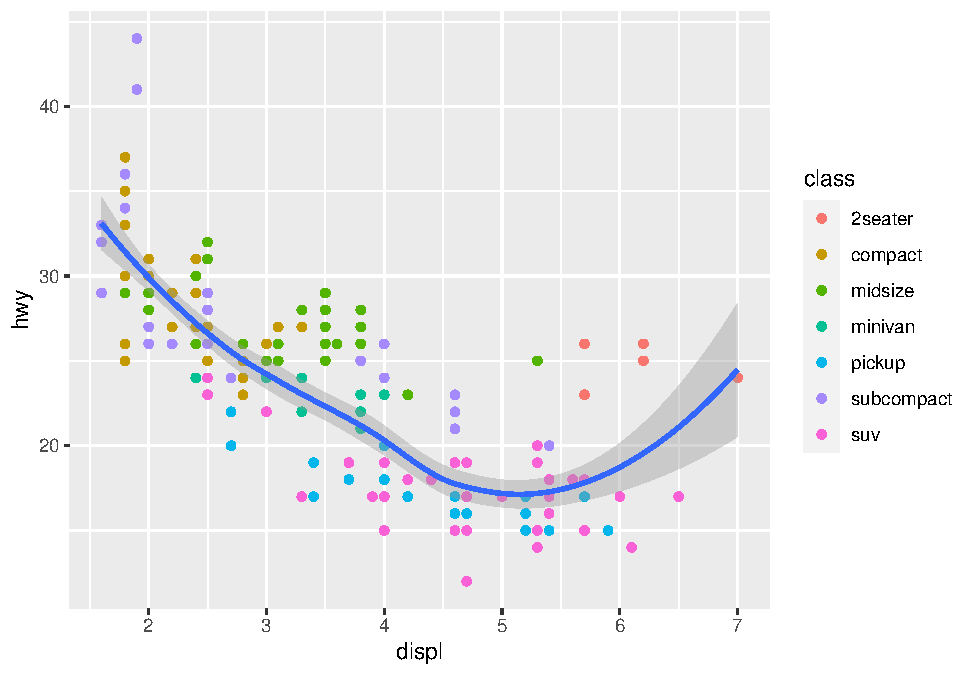
\includegraphics{Journal_files/figure-latex/unnamed-chunk-43-3.pdf}

\begin{Shaded}
\begin{Highlighting}[]
\FunctionTok{ggplot}\NormalTok{(}\AttributeTok{data =}\NormalTok{ mpg, }\AttributeTok{mapping =} \FunctionTok{aes}\NormalTok{(}\AttributeTok{x =}\NormalTok{ displ, }\AttributeTok{y =}\NormalTok{ hwy)) }\SpecialCharTok{+} 
  \FunctionTok{geom\_point}\NormalTok{(}\AttributeTok{mapping =} \FunctionTok{aes}\NormalTok{(}\AttributeTok{color =}\NormalTok{ class)) }\SpecialCharTok{+} 
  \FunctionTok{geom\_smooth}\NormalTok{(}\AttributeTok{data =} \FunctionTok{filter}\NormalTok{(mpg, class }\SpecialCharTok{==} \StringTok{"subcompact"}\NormalTok{), }\AttributeTok{se =} \ConstantTok{FALSE}\NormalTok{)}
\end{Highlighting}
\end{Shaded}

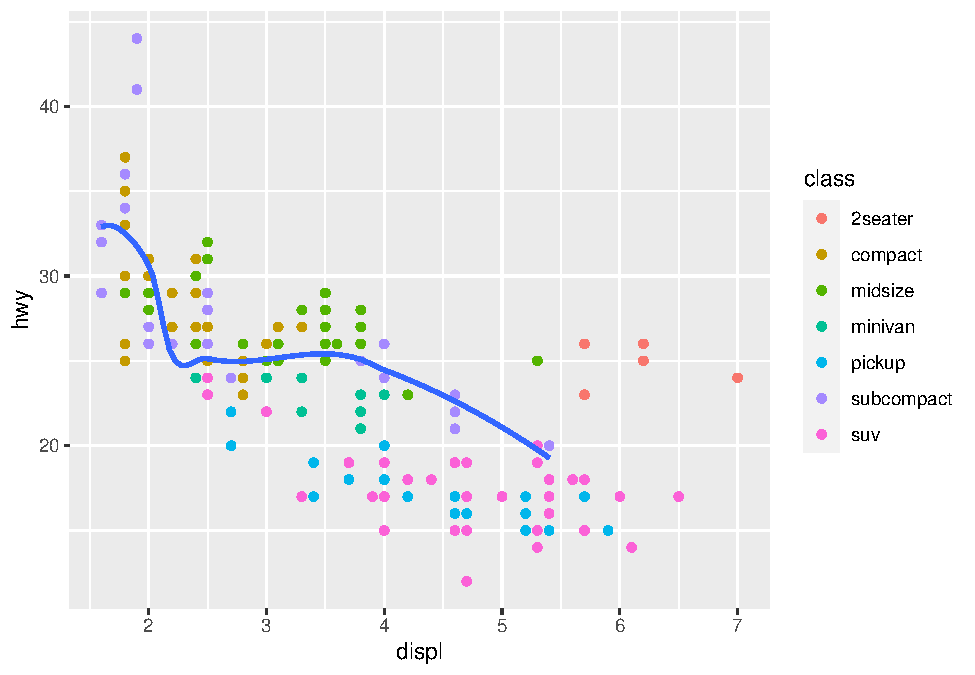
\includegraphics{Journal_files/figure-latex/unnamed-chunk-43-4.pdf} So
we can change mapping such that there are layer of aesthetics (helps us
specify data in labels). We can also modify the plot such that our
object will only mend to some of the data.

\begin{Shaded}
\begin{Highlighting}[]
\FunctionTok{ggplot}\NormalTok{(}\AttributeTok{data =}\NormalTok{ diamonds) }\SpecialCharTok{+} 
  \FunctionTok{geom\_bar}\NormalTok{(}\AttributeTok{mapping =} \FunctionTok{aes}\NormalTok{(}\AttributeTok{x =}\NormalTok{ cut))}
\end{Highlighting}
\end{Shaded}

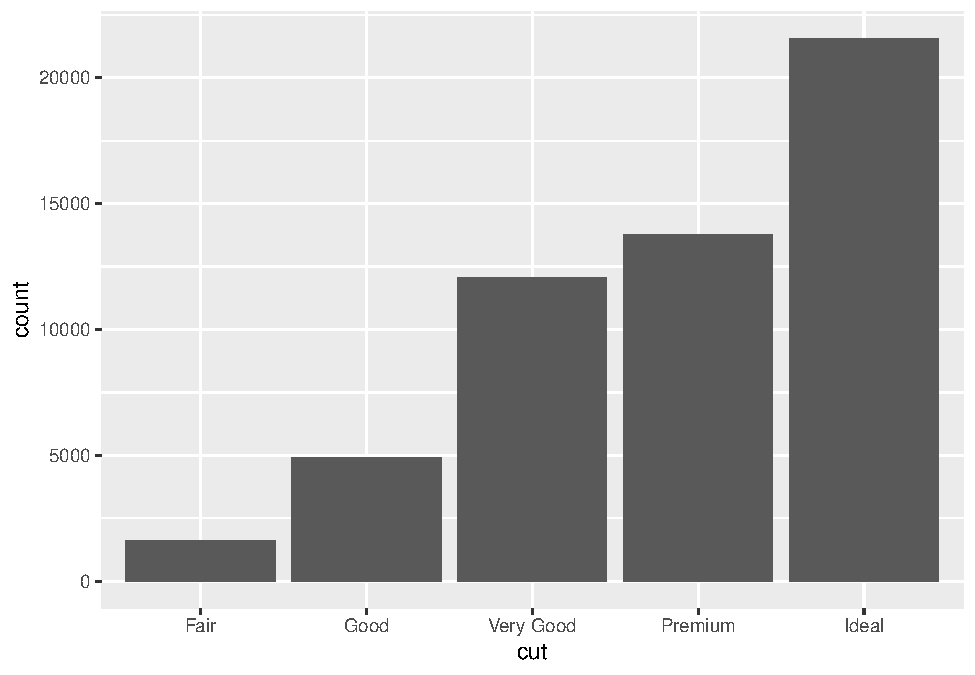
\includegraphics{Journal_files/figure-latex/unnamed-chunk-44-1.pdf}

\begin{Shaded}
\begin{Highlighting}[]
\FunctionTok{ggplot}\NormalTok{(}\AttributeTok{data =}\NormalTok{ diamonds) }\SpecialCharTok{+} 
  \FunctionTok{stat\_count}\NormalTok{(}\AttributeTok{mapping =} \FunctionTok{aes}\NormalTok{(}\AttributeTok{x =}\NormalTok{ cut))}
\end{Highlighting}
\end{Shaded}

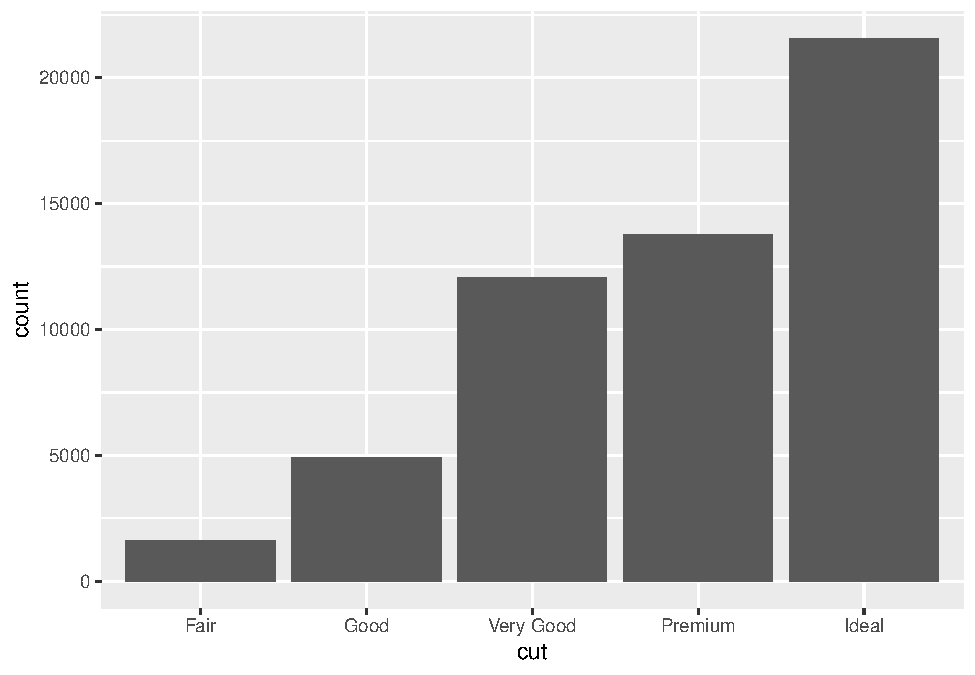
\includegraphics{Journal_files/figure-latex/unnamed-chunk-44-2.pdf}

A simple barplot where the data is grouped by cut. You can use
stat\_count and geom\_bar interchangably since geom\_bar has a default
stat\_count.

\begin{Shaded}
\begin{Highlighting}[]
\NormalTok{demo }\OtherTok{\textless{}{-}} \FunctionTok{tribble}\NormalTok{(}
  \SpecialCharTok{\textasciitilde{}}\NormalTok{cut,         }\SpecialCharTok{\textasciitilde{}}\NormalTok{freq,}
  \StringTok{"Fair"}\NormalTok{,       }\DecValTok{1610}\NormalTok{,}
  \StringTok{"Good"}\NormalTok{,       }\DecValTok{4906}\NormalTok{,}
  \StringTok{"Very Good"}\NormalTok{,  }\DecValTok{12082}\NormalTok{,}
  \StringTok{"Premium"}\NormalTok{,    }\DecValTok{13791}\NormalTok{,}
  \StringTok{"Ideal"}\NormalTok{,      }\DecValTok{21551}
\NormalTok{)}

\FunctionTok{ggplot}\NormalTok{(}\AttributeTok{data =}\NormalTok{ demo) }\SpecialCharTok{+}
  \FunctionTok{geom\_bar}\NormalTok{(}\AttributeTok{mapping =} \FunctionTok{aes}\NormalTok{(}\AttributeTok{x =}\NormalTok{ cut, }\AttributeTok{y =}\NormalTok{ freq), }\AttributeTok{stat =} \StringTok{"identity"}\NormalTok{)}
\end{Highlighting}
\end{Shaded}

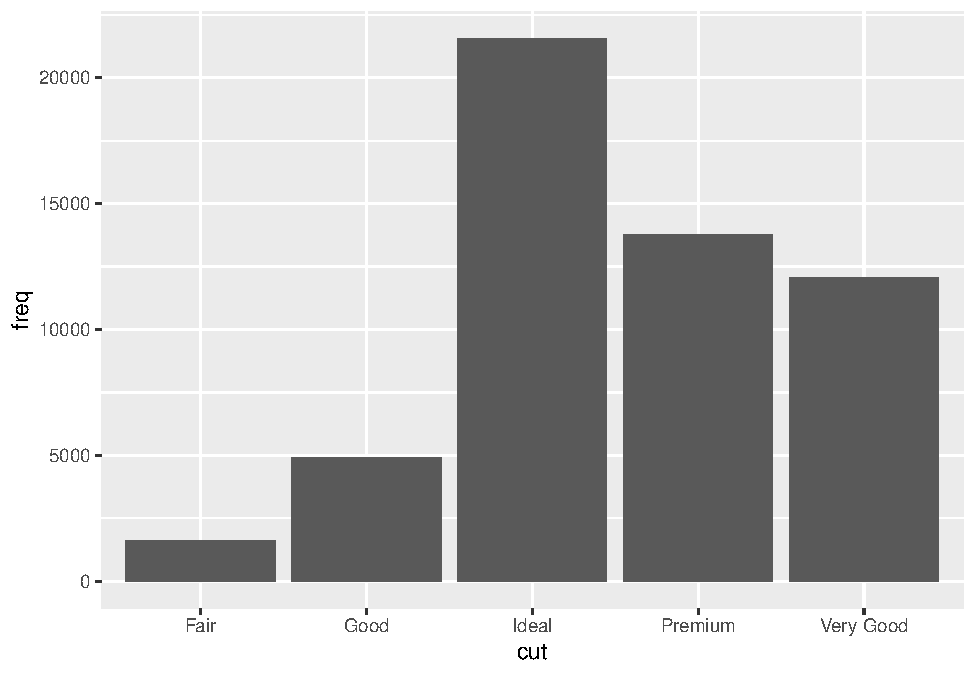
\includegraphics{Journal_files/figure-latex/unnamed-chunk-45-1.pdf} You
can also change the stat count.

\begin{Shaded}
\begin{Highlighting}[]
\FunctionTok{ggplot}\NormalTok{(}\AttributeTok{data =}\NormalTok{ diamonds) }\SpecialCharTok{+} 
  \FunctionTok{geom\_bar}\NormalTok{(}\AttributeTok{mapping =} \FunctionTok{aes}\NormalTok{(}\AttributeTok{x =}\NormalTok{ cut, }\AttributeTok{y =} \FunctionTok{stat}\NormalTok{(prop), }\AttributeTok{group =} \DecValTok{1}\NormalTok{))}
\end{Highlighting}
\end{Shaded}

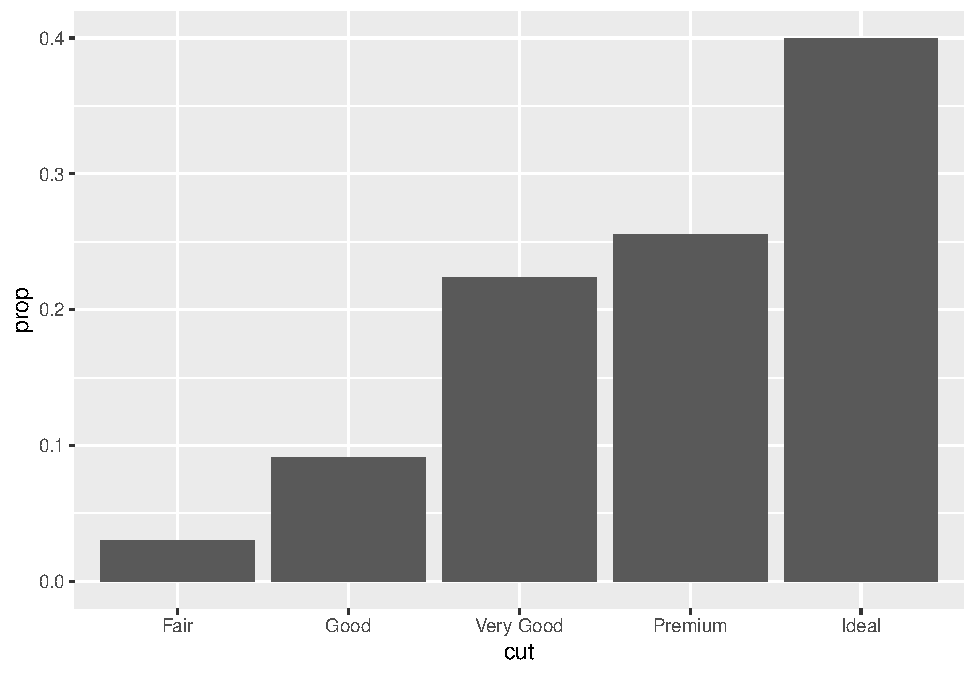
\includegraphics{Journal_files/figure-latex/unnamed-chunk-46-1.pdf}

You might want to override the default mapping from transformed
variables to aesthetics. For example, you might want to display a bar
chart of proportion, rather than count:

\begin{Shaded}
\begin{Highlighting}[]
\FunctionTok{ggplot}\NormalTok{(}\AttributeTok{data =}\NormalTok{ diamonds) }\SpecialCharTok{+} 
  \FunctionTok{stat\_summary}\NormalTok{(}
    \AttributeTok{mapping =} \FunctionTok{aes}\NormalTok{(}\AttributeTok{x =}\NormalTok{ cut, }\AttributeTok{y =}\NormalTok{ depth),}
    \AttributeTok{fun.min =}\NormalTok{ min,}
    \AttributeTok{fun.max =}\NormalTok{ max,}
    \AttributeTok{fun =}\NormalTok{ median}
\NormalTok{  )}
\end{Highlighting}
\end{Shaded}

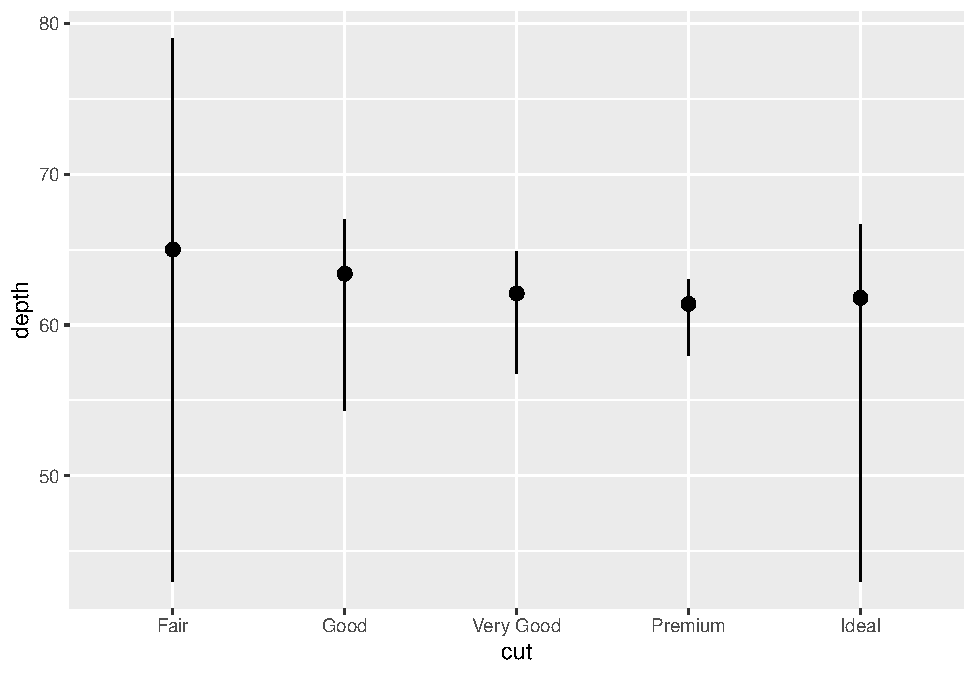
\includegraphics{Journal_files/figure-latex/unnamed-chunk-47-1.pdf}

we can do it for a transformation on statisitcs aswell where we take a
stat summary and take the specific val of each category.

\begin{Shaded}
\begin{Highlighting}[]
\FunctionTok{ggplot}\NormalTok{(}\AttributeTok{data =}\NormalTok{ diamonds) }\SpecialCharTok{+} 
  \FunctionTok{geom\_bar}\NormalTok{(}\AttributeTok{mapping =} \FunctionTok{aes}\NormalTok{(}\AttributeTok{x =}\NormalTok{ cut, }\AttributeTok{colour =}\NormalTok{ cut))}
\end{Highlighting}
\end{Shaded}

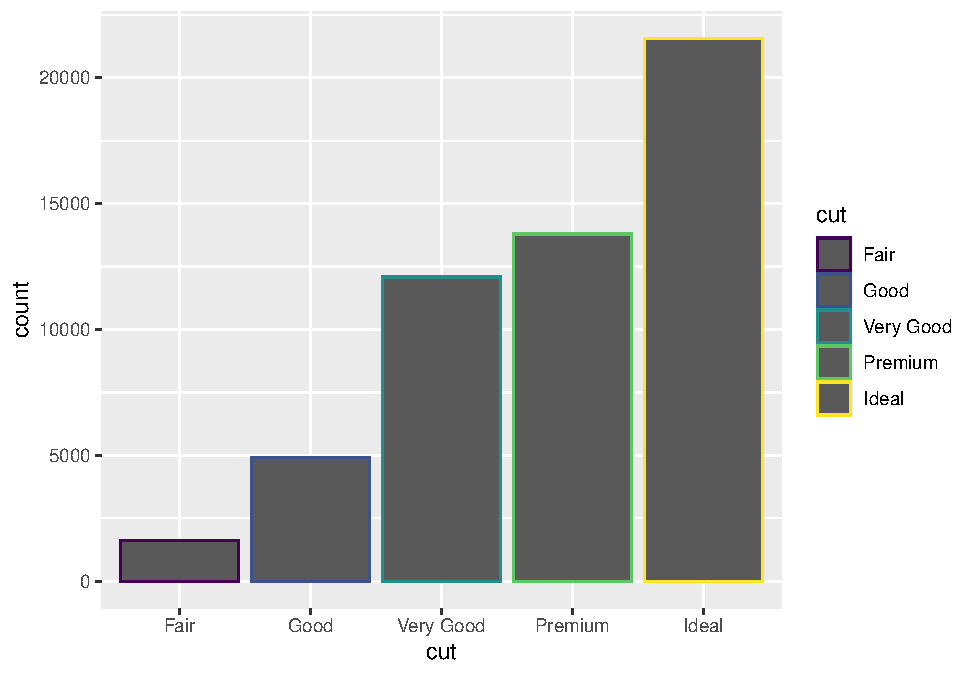
\includegraphics{Journal_files/figure-latex/unnamed-chunk-48-1.pdf}

\begin{Shaded}
\begin{Highlighting}[]
\FunctionTok{ggplot}\NormalTok{(}\AttributeTok{data =}\NormalTok{ diamonds) }\SpecialCharTok{+} 
  \FunctionTok{geom\_bar}\NormalTok{(}\AttributeTok{mapping =} \FunctionTok{aes}\NormalTok{(}\AttributeTok{x =}\NormalTok{ cut, }\AttributeTok{fill =}\NormalTok{ cut))}
\end{Highlighting}
\end{Shaded}

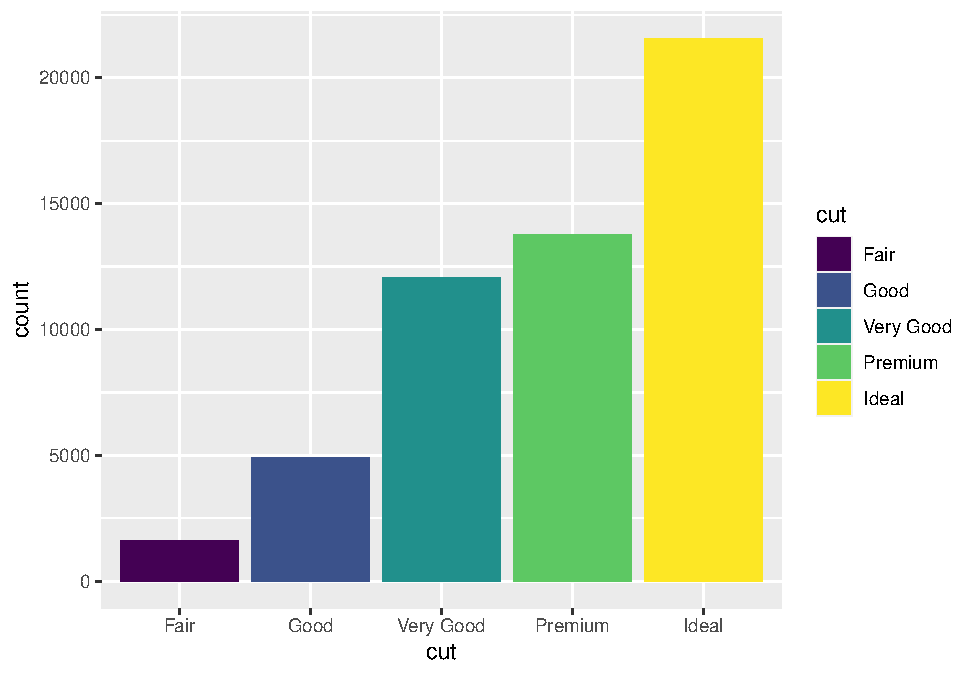
\includegraphics{Journal_files/figure-latex/unnamed-chunk-48-2.pdf}

\begin{Shaded}
\begin{Highlighting}[]
\FunctionTok{ggplot}\NormalTok{(}\AttributeTok{data =}\NormalTok{ diamonds) }\SpecialCharTok{+} 
  \FunctionTok{geom\_bar}\NormalTok{(}\AttributeTok{mapping =} \FunctionTok{aes}\NormalTok{(}\AttributeTok{x =}\NormalTok{ cut, }\AttributeTok{fill =}\NormalTok{ clarity))}
\end{Highlighting}
\end{Shaded}

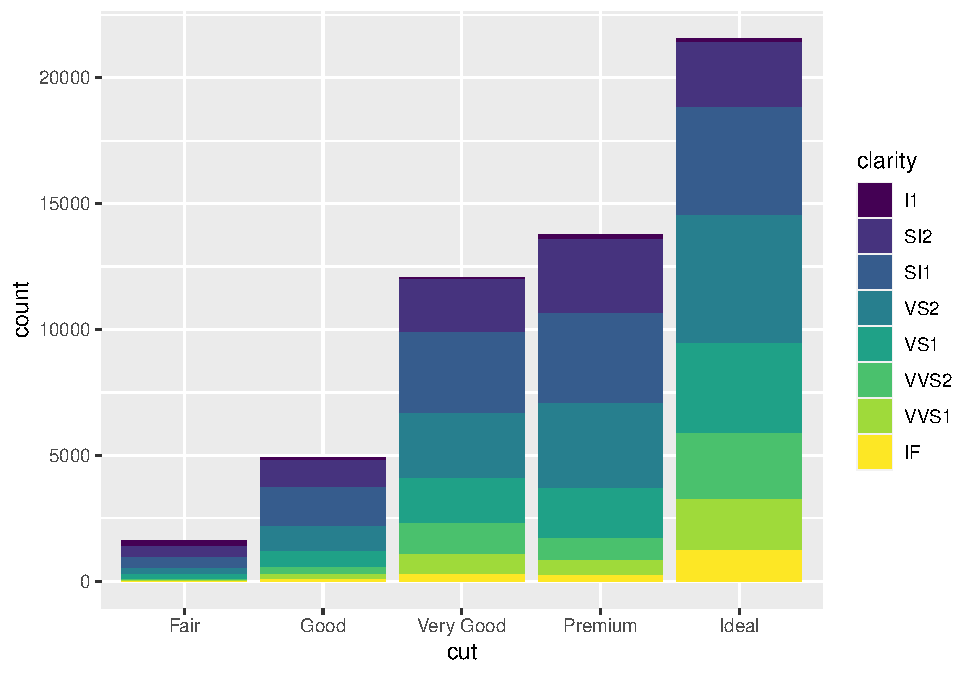
\includegraphics{Journal_files/figure-latex/unnamed-chunk-48-3.pdf}

\begin{Shaded}
\begin{Highlighting}[]
\FunctionTok{ggplot}\NormalTok{(}\AttributeTok{data =}\NormalTok{ diamonds, }\AttributeTok{mapping =} \FunctionTok{aes}\NormalTok{(}\AttributeTok{x =}\NormalTok{ cut, }\AttributeTok{fill =}\NormalTok{ clarity)) }\SpecialCharTok{+} 
  \FunctionTok{geom\_bar}\NormalTok{(}\AttributeTok{alpha =} \DecValTok{1}\SpecialCharTok{/}\DecValTok{5}\NormalTok{, }\AttributeTok{position =} \StringTok{"identity"}\NormalTok{)}
\end{Highlighting}
\end{Shaded}

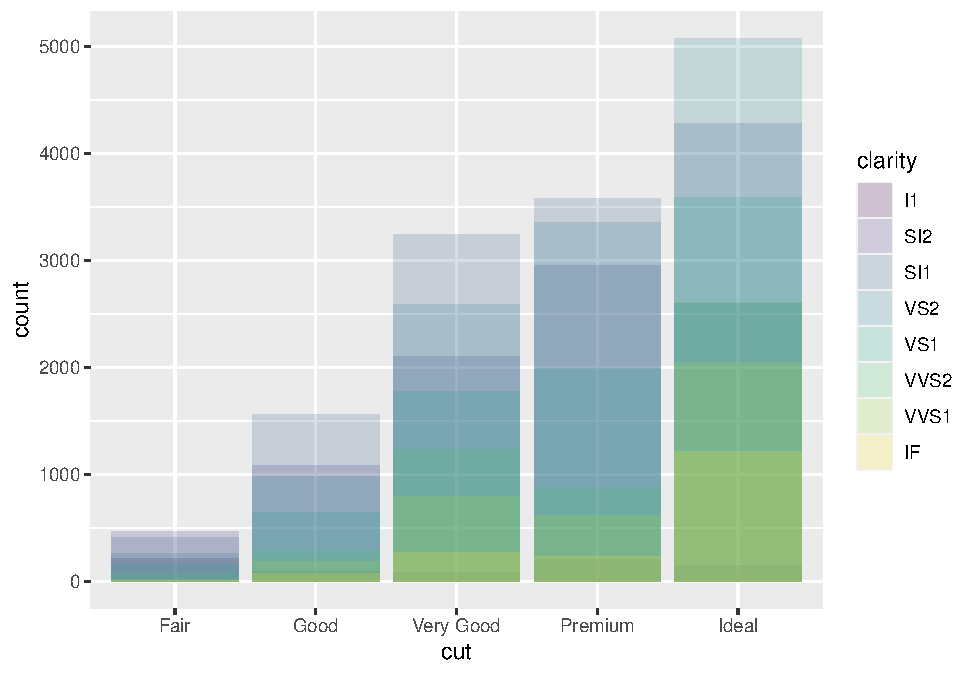
\includegraphics{Journal_files/figure-latex/unnamed-chunk-48-4.pdf}

\begin{Shaded}
\begin{Highlighting}[]
\FunctionTok{ggplot}\NormalTok{(}\AttributeTok{data =}\NormalTok{ diamonds, }\AttributeTok{mapping =} \FunctionTok{aes}\NormalTok{(}\AttributeTok{x =}\NormalTok{ cut, }\AttributeTok{colour =}\NormalTok{ clarity)) }\SpecialCharTok{+} 
  \FunctionTok{geom\_bar}\NormalTok{(}\AttributeTok{fill =} \ConstantTok{NA}\NormalTok{, }\AttributeTok{position =} \StringTok{"identity"}\NormalTok{)}
\end{Highlighting}
\end{Shaded}

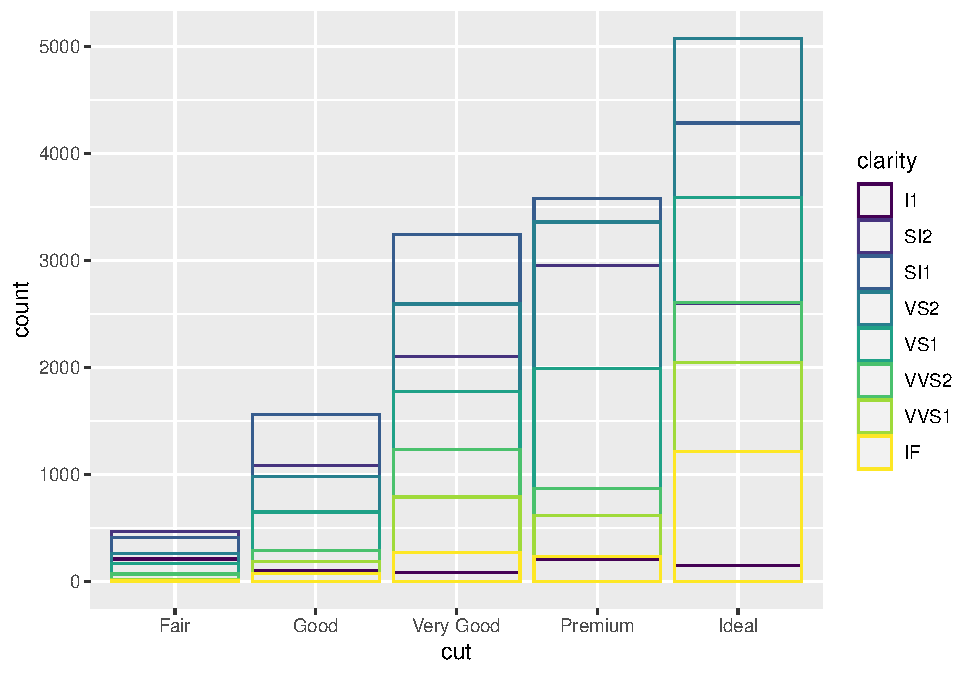
\includegraphics{Journal_files/figure-latex/unnamed-chunk-48-5.pdf} Now,
we can change the position such that they can either overlap on each
other and see something special about the data.

\begin{Shaded}
\begin{Highlighting}[]
\FunctionTok{ggplot}\NormalTok{(}\AttributeTok{data =}\NormalTok{ diamonds) }\SpecialCharTok{+} 
  \FunctionTok{geom\_bar}\NormalTok{(}\AttributeTok{mapping =} \FunctionTok{aes}\NormalTok{(}\AttributeTok{x =}\NormalTok{ cut, }\AttributeTok{fill =}\NormalTok{ clarity), }\AttributeTok{position =} \StringTok{"fill"}\NormalTok{)}
\end{Highlighting}
\end{Shaded}

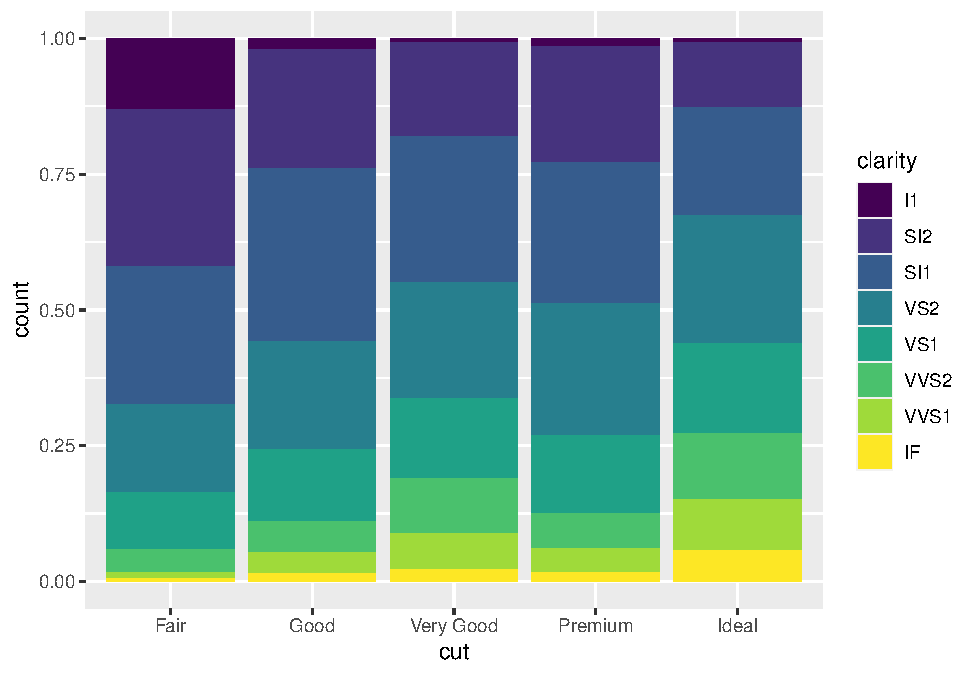
\includegraphics{Journal_files/figure-latex/unnamed-chunk-49-1.pdf}

\begin{Shaded}
\begin{Highlighting}[]
\FunctionTok{ggplot}\NormalTok{(}\AttributeTok{data =}\NormalTok{ diamonds) }\SpecialCharTok{+} 
  \FunctionTok{geom\_bar}\NormalTok{(}\AttributeTok{mapping =} \FunctionTok{aes}\NormalTok{(}\AttributeTok{x =}\NormalTok{ cut, }\AttributeTok{fill =}\NormalTok{ clarity), }\AttributeTok{position =} \StringTok{"dodge"}\NormalTok{)}
\end{Highlighting}
\end{Shaded}

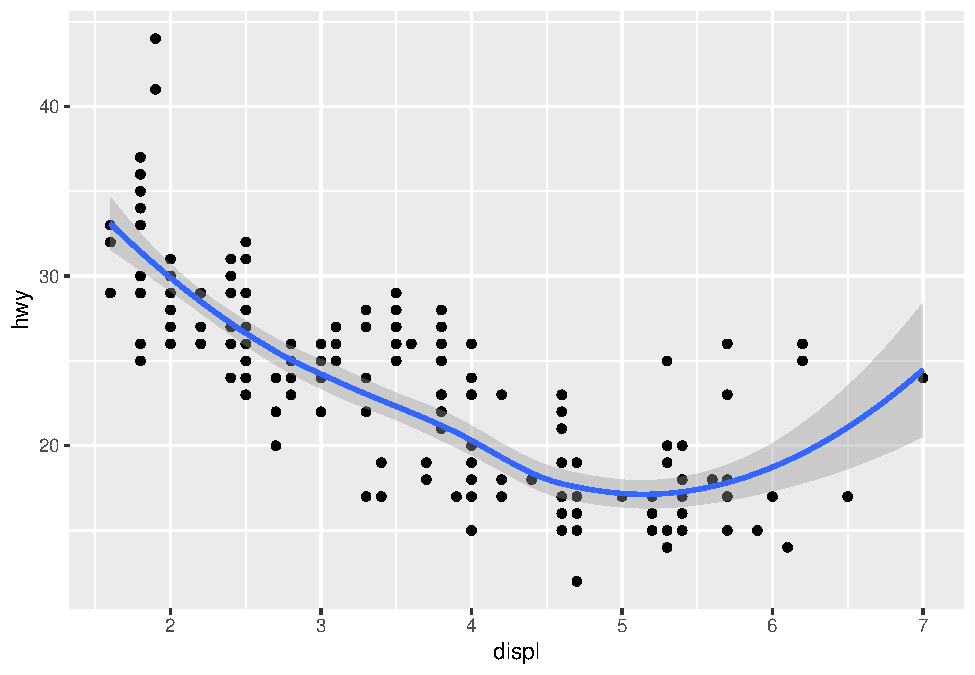
\includegraphics{Journal_files/figure-latex/unnamed-chunk-49-2.pdf} We
can use things like position to see proportion to data or dodge to
overlap them.

\begin{Shaded}
\begin{Highlighting}[]
\FunctionTok{ggplot}\NormalTok{(}\AttributeTok{data =}\NormalTok{ mpg) }\SpecialCharTok{+} 
  \FunctionTok{geom\_point}\NormalTok{(}\AttributeTok{mapping =} \FunctionTok{aes}\NormalTok{(}\AttributeTok{x =}\NormalTok{ displ, }\AttributeTok{y =}\NormalTok{ hwy), }\AttributeTok{position =} \StringTok{"jitter"}\NormalTok{)}
\end{Highlighting}
\end{Shaded}

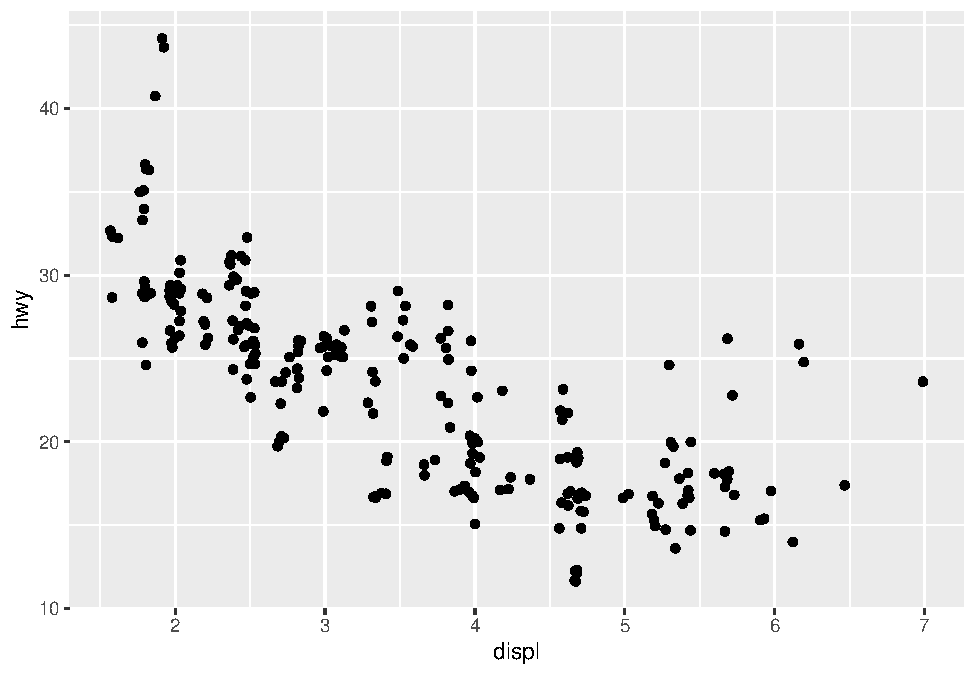
\includegraphics{Journal_files/figure-latex/unnamed-chunk-50-1.pdf} We
can change our data such that their isn't overplotting such that the
arrangement is now easier to see.

The template for all this is:

ggplot(data = ) + ( mapping = aes(), stat = , position = ) + +

``To see this, let's add position adjustments, stats, coordinate
systems, and faceting to our code template:''

\hypertarget{graphics-for-communication}{%
\subsection{Graphics for
communication}\label{graphics-for-communication}}

\begin{Shaded}
\begin{Highlighting}[]
\FunctionTok{ggplot}\NormalTok{(mpg, }\FunctionTok{aes}\NormalTok{(displ, hwy)) }\SpecialCharTok{+}
  \FunctionTok{geom\_point}\NormalTok{(}\FunctionTok{aes}\NormalTok{(}\AttributeTok{color =}\NormalTok{ class)) }\SpecialCharTok{+}
  \FunctionTok{geom\_smooth}\NormalTok{(}\AttributeTok{se =} \ConstantTok{FALSE}\NormalTok{) }\SpecialCharTok{+}
  \FunctionTok{labs}\NormalTok{(}\AttributeTok{title =} \StringTok{"Fuel efficiency generally decreases with engine size"}\NormalTok{)}
\end{Highlighting}
\end{Shaded}

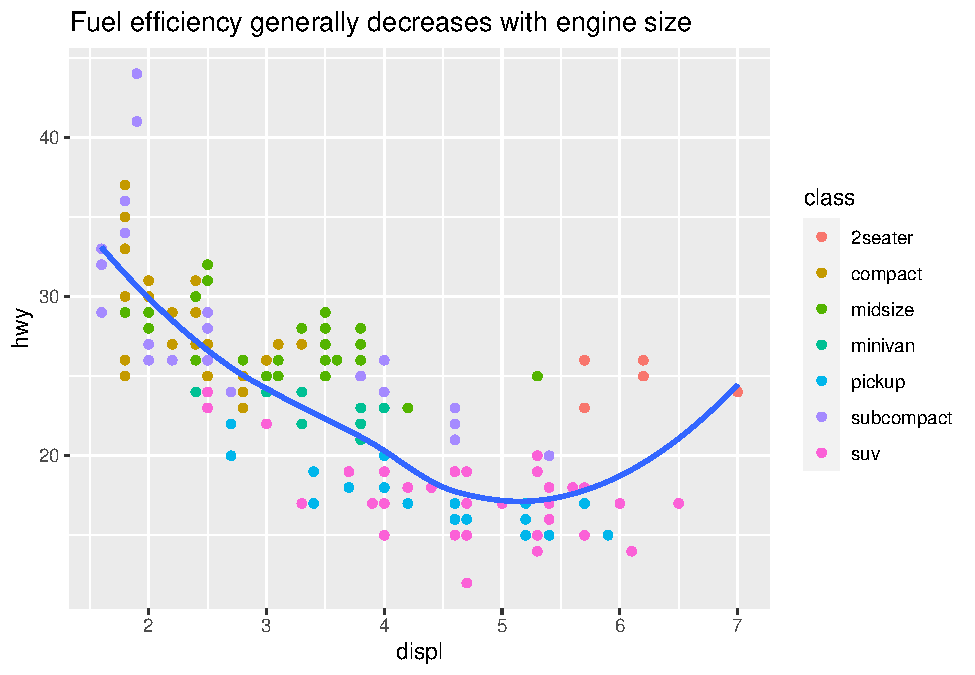
\includegraphics{Journal_files/figure-latex/unnamed-chunk-51-1.pdf}

\begin{Shaded}
\begin{Highlighting}[]
\FunctionTok{ggplot}\NormalTok{(mpg, }\FunctionTok{aes}\NormalTok{(displ, hwy)) }\SpecialCharTok{+}
  \FunctionTok{geom\_point}\NormalTok{(}\FunctionTok{aes}\NormalTok{(}\AttributeTok{color =}\NormalTok{ class)) }\SpecialCharTok{+}
  \FunctionTok{geom\_smooth}\NormalTok{(}\AttributeTok{se =} \ConstantTok{FALSE}\NormalTok{) }\SpecialCharTok{+}
  \FunctionTok{labs}\NormalTok{(}
    \AttributeTok{title =} \StringTok{"Fuel efficiency generally decreases with engine size"}\NormalTok{,}
    \AttributeTok{subtitle =} \StringTok{"Two seaters (sports cars) are an exception because of their light weight"}\NormalTok{,}
    \AttributeTok{caption =} \StringTok{"Data from fueleconomy.gov"}
\NormalTok{  )}
\end{Highlighting}
\end{Shaded}

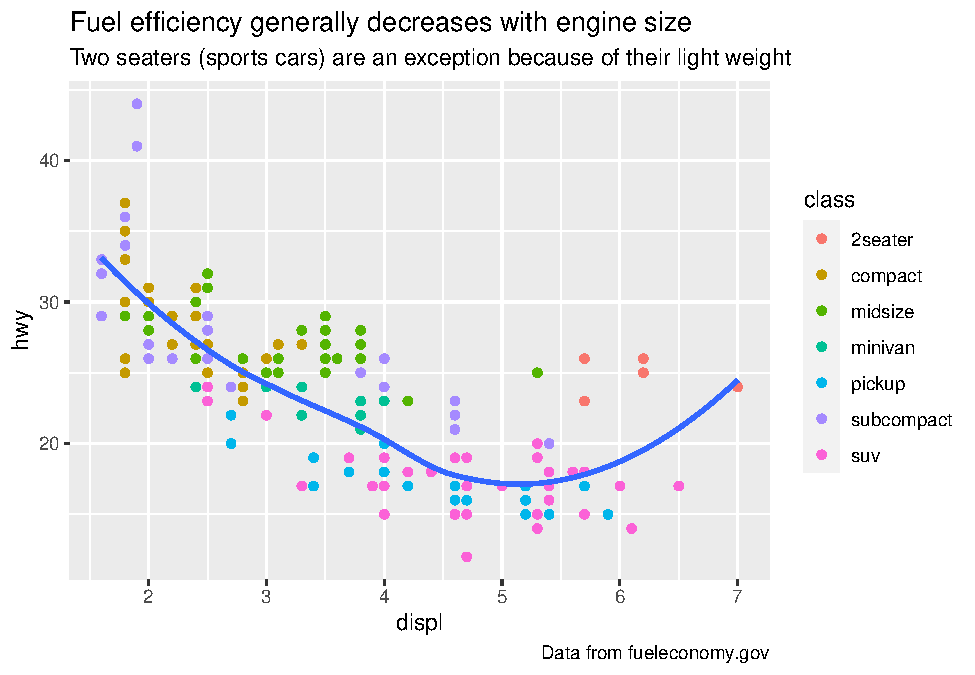
\includegraphics{Journal_files/figure-latex/unnamed-chunk-51-2.pdf}

\begin{Shaded}
\begin{Highlighting}[]
\FunctionTok{ggplot}\NormalTok{(mpg, }\FunctionTok{aes}\NormalTok{(displ, hwy)) }\SpecialCharTok{+}
  \FunctionTok{geom\_point}\NormalTok{(}\FunctionTok{aes}\NormalTok{(}\AttributeTok{colour =}\NormalTok{ class)) }\SpecialCharTok{+}
  \FunctionTok{geom\_smooth}\NormalTok{(}\AttributeTok{se =} \ConstantTok{FALSE}\NormalTok{) }\SpecialCharTok{+}
  \FunctionTok{labs}\NormalTok{(}
    \AttributeTok{x =} \StringTok{"Engine displacement (L)"}\NormalTok{,}
    \AttributeTok{y =} \StringTok{"Highway fuel economy (mpg)"}\NormalTok{,}
    \AttributeTok{colour =} \StringTok{"Car type"}
\NormalTok{  )}
\end{Highlighting}
\end{Shaded}

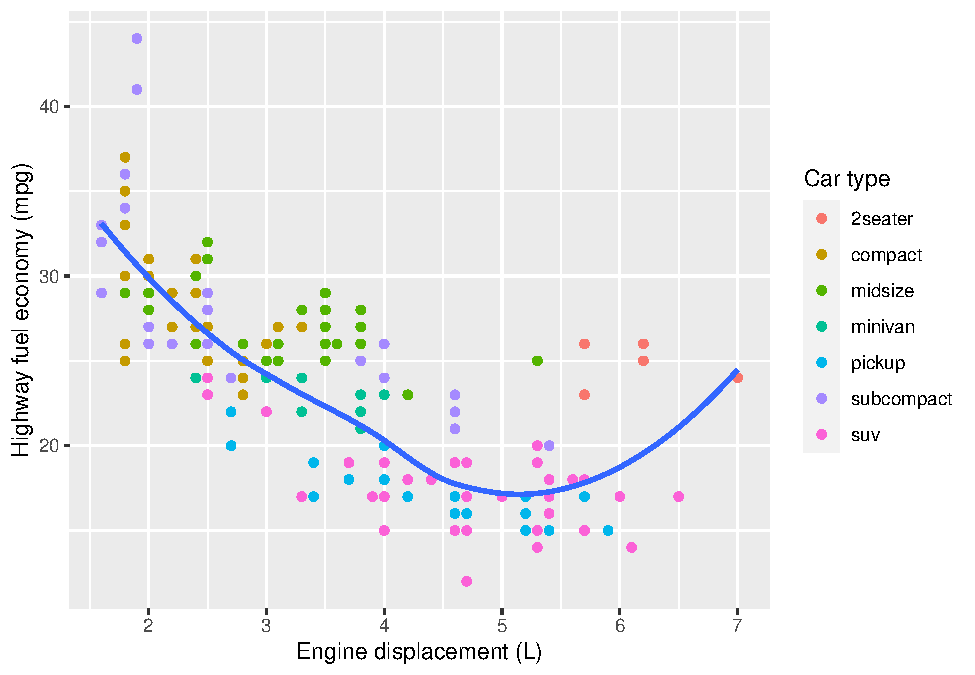
\includegraphics{Journal_files/figure-latex/unnamed-chunk-51-3.pdf}

\begin{Shaded}
\begin{Highlighting}[]
\NormalTok{df }\OtherTok{\textless{}{-}} \FunctionTok{tibble}\NormalTok{(}
  \AttributeTok{x =} \FunctionTok{runif}\NormalTok{(}\DecValTok{10}\NormalTok{),}
  \AttributeTok{y =} \FunctionTok{runif}\NormalTok{(}\DecValTok{10}\NormalTok{)}
\NormalTok{)}
\FunctionTok{ggplot}\NormalTok{(df, }\FunctionTok{aes}\NormalTok{(x, y)) }\SpecialCharTok{+}
  \FunctionTok{geom\_point}\NormalTok{() }\SpecialCharTok{+}
  \FunctionTok{labs}\NormalTok{(}
    \AttributeTok{x =} \FunctionTok{quote}\NormalTok{(}\FunctionTok{sum}\NormalTok{(x[i] }\SpecialCharTok{\^{}} \DecValTok{2}\NormalTok{, i }\SpecialCharTok{==} \DecValTok{1}\NormalTok{, n)),}
    \AttributeTok{y =} \FunctionTok{quote}\NormalTok{(alpha }\SpecialCharTok{+}\NormalTok{ beta }\SpecialCharTok{+} \FunctionTok{frac}\NormalTok{(delta, theta))}
\NormalTok{  )}
\end{Highlighting}
\end{Shaded}

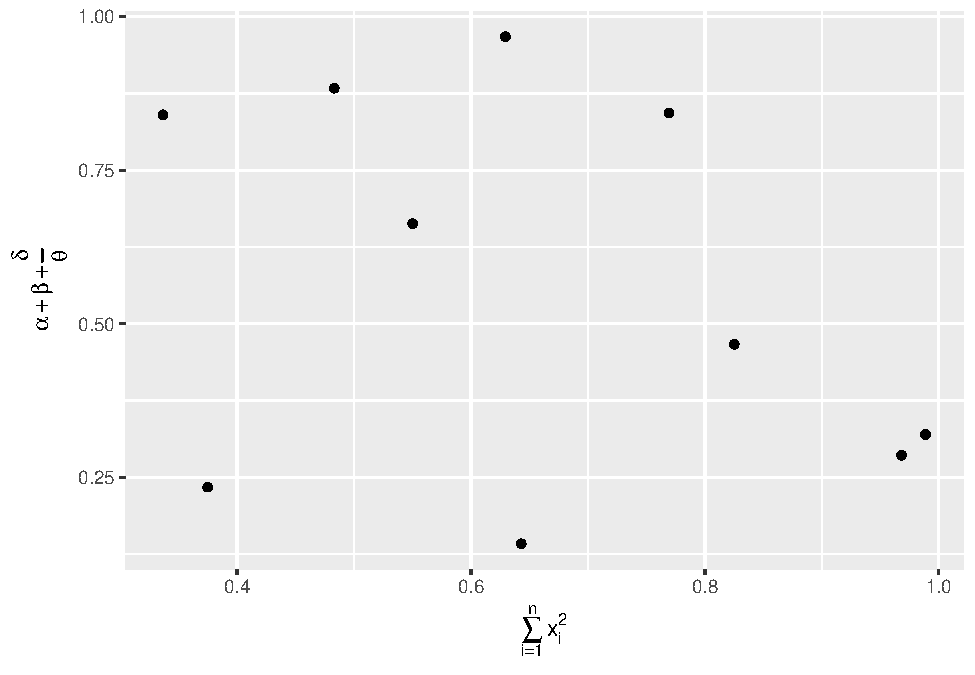
\includegraphics{Journal_files/figure-latex/unnamed-chunk-51-4.pdf} We
can put labels in places like the title. You can also add them as
subtitles, captions, x, and y. Labels can even be written as
mathematical equations.

You can take it a step further and make annotations for specific points

\begin{Shaded}
\begin{Highlighting}[]
\NormalTok{best\_in\_class }\OtherTok{\textless{}{-}}\NormalTok{ mpg }\SpecialCharTok{\%\textgreater{}\%}
  \FunctionTok{group\_by}\NormalTok{(class) }\SpecialCharTok{\%\textgreater{}\%}
  \FunctionTok{filter}\NormalTok{(}\FunctionTok{row\_number}\NormalTok{(}\FunctionTok{desc}\NormalTok{(hwy)) }\SpecialCharTok{==} \DecValTok{1}\NormalTok{)}

\FunctionTok{ggplot}\NormalTok{(mpg, }\FunctionTok{aes}\NormalTok{(displ, hwy)) }\SpecialCharTok{+}
  \FunctionTok{geom\_point}\NormalTok{(}\FunctionTok{aes}\NormalTok{(}\AttributeTok{colour =}\NormalTok{ class)) }\SpecialCharTok{+}
  \FunctionTok{geom\_text}\NormalTok{(}\FunctionTok{aes}\NormalTok{(}\AttributeTok{label =}\NormalTok{ model), }\AttributeTok{data =}\NormalTok{ best\_in\_class)}
\end{Highlighting}
\end{Shaded}

\includegraphics{Journal_files/figure-latex/unnamed-chunk-52-1.pdf}

\begin{Shaded}
\begin{Highlighting}[]
\FunctionTok{ggplot}\NormalTok{(mpg, }\FunctionTok{aes}\NormalTok{(displ, hwy)) }\SpecialCharTok{+}
  \FunctionTok{geom\_point}\NormalTok{(}\FunctionTok{aes}\NormalTok{(}\AttributeTok{colour =}\NormalTok{ class)) }\SpecialCharTok{+}
  \FunctionTok{geom\_label}\NormalTok{(}\FunctionTok{aes}\NormalTok{(}\AttributeTok{label =}\NormalTok{ model), }\AttributeTok{data =}\NormalTok{ best\_in\_class, }\AttributeTok{nudge\_y =} \DecValTok{2}\NormalTok{, }\AttributeTok{alpha =} \FloatTok{0.5}\NormalTok{)}
\end{Highlighting}
\end{Shaded}

\includegraphics{Journal_files/figure-latex/unnamed-chunk-52-2.pdf}

\begin{Shaded}
\begin{Highlighting}[]
\FunctionTok{ggplot}\NormalTok{(mpg, }\FunctionTok{aes}\NormalTok{(displ, hwy)) }\SpecialCharTok{+}
  \FunctionTok{geom\_point}\NormalTok{(}\FunctionTok{aes}\NormalTok{(}\AttributeTok{colour =}\NormalTok{ class)) }\SpecialCharTok{+}
  \FunctionTok{geom\_point}\NormalTok{(}\AttributeTok{size =} \DecValTok{3}\NormalTok{, }\AttributeTok{shape =} \DecValTok{1}\NormalTok{, }\AttributeTok{data =}\NormalTok{ best\_in\_class) }\SpecialCharTok{+}
\NormalTok{  ggrepel}\SpecialCharTok{::}\FunctionTok{geom\_label\_repel}\NormalTok{(}\FunctionTok{aes}\NormalTok{(}\AttributeTok{label =}\NormalTok{ model), }\AttributeTok{data =}\NormalTok{ best\_in\_class)}
\end{Highlighting}
\end{Shaded}

\includegraphics{Journal_files/figure-latex/unnamed-chunk-52-3.pdf} In
this graph, we label the cars that are the best in their class in terms
of mpg.

The label is hard to read from one another, so we can modify it such
that it is easier to see. Additionally, if you use ggrepel then you can
make it so the labels are not right on top of each other.

\begin{Shaded}
\begin{Highlighting}[]
\NormalTok{class\_avg }\OtherTok{\textless{}{-}}\NormalTok{ mpg }\SpecialCharTok{\%\textgreater{}\%}
  \FunctionTok{group\_by}\NormalTok{(class) }\SpecialCharTok{\%\textgreater{}\%}
  \FunctionTok{summarise}\NormalTok{(}
    \AttributeTok{displ =} \FunctionTok{median}\NormalTok{(displ),}
    \AttributeTok{hwy =} \FunctionTok{median}\NormalTok{(hwy)}
\NormalTok{  )}
\CommentTok{\#\textgreater{} \textasciigrave{}summarise()\textasciigrave{} ungrouping output (override with \textasciigrave{}.groups\textasciigrave{} argument)}

\FunctionTok{ggplot}\NormalTok{(mpg, }\FunctionTok{aes}\NormalTok{(displ, hwy, }\AttributeTok{colour =}\NormalTok{ class)) }\SpecialCharTok{+}
\NormalTok{  ggrepel}\SpecialCharTok{::}\FunctionTok{geom\_label\_repel}\NormalTok{(}\FunctionTok{aes}\NormalTok{(}\AttributeTok{label =}\NormalTok{ class),}
    \AttributeTok{data =}\NormalTok{ class\_avg,}
    \AttributeTok{size =} \DecValTok{6}\NormalTok{,}
    \AttributeTok{label.size =} \DecValTok{0}\NormalTok{,}
    \AttributeTok{segment.color =} \ConstantTok{NA}
\NormalTok{  ) }\SpecialCharTok{+}
  \FunctionTok{geom\_point}\NormalTok{() }\SpecialCharTok{+}
  \FunctionTok{theme}\NormalTok{(}\AttributeTok{legend.position =} \StringTok{"none"}\NormalTok{)}
\end{Highlighting}
\end{Shaded}

\includegraphics{Journal_files/figure-latex/unnamed-chunk-53-1.pdf}

\begin{Shaded}
\begin{Highlighting}[]
\NormalTok{label }\OtherTok{\textless{}{-}}\NormalTok{ mpg }\SpecialCharTok{\%\textgreater{}\%}
  \FunctionTok{summarise}\NormalTok{(}
    \AttributeTok{displ =} \FunctionTok{max}\NormalTok{(displ),}
    \AttributeTok{hwy =} \FunctionTok{max}\NormalTok{(hwy),}
    \AttributeTok{label =} \StringTok{"Increasing engine size is }\SpecialCharTok{\textbackslash{}n}\StringTok{related to decreasing fuel economy."}
\NormalTok{  )}

\FunctionTok{ggplot}\NormalTok{(mpg, }\FunctionTok{aes}\NormalTok{(displ, hwy)) }\SpecialCharTok{+}
  \FunctionTok{geom\_point}\NormalTok{() }\SpecialCharTok{+}
  \FunctionTok{geom\_text}\NormalTok{(}\FunctionTok{aes}\NormalTok{(}\AttributeTok{label =}\NormalTok{ label), }\AttributeTok{data =}\NormalTok{ label, }\AttributeTok{vjust =} \StringTok{"top"}\NormalTok{, }\AttributeTok{hjust =} \StringTok{"right"}\NormalTok{)}
\end{Highlighting}
\end{Shaded}

\includegraphics{Journal_files/figure-latex/unnamed-chunk-53-2.pdf}

\begin{Shaded}
\begin{Highlighting}[]
\NormalTok{label }\OtherTok{\textless{}{-}} \FunctionTok{tibble}\NormalTok{(}
  \AttributeTok{displ =} \ConstantTok{Inf}\NormalTok{,}
  \AttributeTok{hwy =} \ConstantTok{Inf}\NormalTok{,}
  \AttributeTok{label =} \StringTok{"Increasing engine size is }\SpecialCharTok{\textbackslash{}n}\StringTok{related to decreasing fuel economy."}
\NormalTok{)}

\FunctionTok{ggplot}\NormalTok{(mpg, }\FunctionTok{aes}\NormalTok{(displ, hwy)) }\SpecialCharTok{+}
  \FunctionTok{geom\_point}\NormalTok{() }\SpecialCharTok{+}
  \FunctionTok{geom\_text}\NormalTok{(}\FunctionTok{aes}\NormalTok{(}\AttributeTok{label =}\NormalTok{ label), }\AttributeTok{data =}\NormalTok{ label, }\AttributeTok{vjust =} \StringTok{"top"}\NormalTok{, }\AttributeTok{hjust =} \StringTok{"right"}\NormalTok{)}
\end{Highlighting}
\end{Shaded}

\includegraphics{Journal_files/figure-latex/unnamed-chunk-53-3.pdf} We
can turn the legend off and then put annotations near the colors such
that they represent what each car type is. Additionally, you can just
add a single label to the plot and then write what you want.

If you want to place text exactly where the borders are then you can use
INF(which can be positive or negative).

There are nine different possibilities for locations that labels can go
in (NESW).

Use geom\_hline() and geom\_vline() to add reference lines. I often make
them thick (size = 2) and white (colour = white), and draw them
underneath the primary data layer. That makes them easy to see, without
drawing attention away from the data.

Use geom\_rect() to draw a rectangle around points of interest. The
boundaries of the rectangle are defined by aesthetics xmin, xmax, ymin,
ymax.

Use geom\_segment() with the arrow argument to draw attention to a point
with an arrow. Use aesthetics x and y to define the starting location,
and xend and yend to define the end location.

\begin{Shaded}
\begin{Highlighting}[]
\FunctionTok{ggplot}\NormalTok{(mpg, }\FunctionTok{aes}\NormalTok{(displ, hwy)) }\SpecialCharTok{+}
  \FunctionTok{geom\_point}\NormalTok{(}\FunctionTok{aes}\NormalTok{(}\AttributeTok{colour =}\NormalTok{ class))}
\end{Highlighting}
\end{Shaded}

\includegraphics{Journal_files/figure-latex/unnamed-chunk-54-1.pdf}

\begin{Shaded}
\begin{Highlighting}[]
\FunctionTok{ggplot}\NormalTok{(mpg, }\FunctionTok{aes}\NormalTok{(displ, hwy)) }\SpecialCharTok{+}
  \FunctionTok{geom\_point}\NormalTok{(}\FunctionTok{aes}\NormalTok{(}\AttributeTok{colour =}\NormalTok{ class)) }\SpecialCharTok{+}
  \FunctionTok{scale\_x\_continuous}\NormalTok{() }\SpecialCharTok{+}
  \FunctionTok{scale\_y\_continuous}\NormalTok{() }\SpecialCharTok{+}
  \FunctionTok{scale\_colour\_discrete}\NormalTok{()}
\end{Highlighting}
\end{Shaded}

\includegraphics{Journal_files/figure-latex/unnamed-chunk-54-2.pdf}

\begin{Shaded}
\begin{Highlighting}[]
\FunctionTok{ggplot}\NormalTok{(mpg, }\FunctionTok{aes}\NormalTok{(displ, hwy)) }\SpecialCharTok{+}
  \FunctionTok{geom\_point}\NormalTok{() }\SpecialCharTok{+}
  \FunctionTok{scale\_y\_continuous}\NormalTok{(}\AttributeTok{breaks =} \FunctionTok{seq}\NormalTok{(}\DecValTok{15}\NormalTok{, }\DecValTok{40}\NormalTok{, }\AttributeTok{by =} \DecValTok{5}\NormalTok{))}
\end{Highlighting}
\end{Shaded}

\includegraphics{Journal_files/figure-latex/unnamed-chunk-54-3.pdf}

\begin{Shaded}
\begin{Highlighting}[]
\FunctionTok{ggplot}\NormalTok{(mpg, }\FunctionTok{aes}\NormalTok{(displ, hwy)) }\SpecialCharTok{+}
  \FunctionTok{geom\_point}\NormalTok{() }\SpecialCharTok{+}
  \FunctionTok{scale\_x\_continuous}\NormalTok{(}\AttributeTok{labels =} \ConstantTok{NULL}\NormalTok{) }\SpecialCharTok{+}
  \FunctionTok{scale\_y\_continuous}\NormalTok{(}\AttributeTok{labels =} \ConstantTok{NULL}\NormalTok{)}
\end{Highlighting}
\end{Shaded}

\includegraphics{Journal_files/figure-latex/unnamed-chunk-54-4.pdf}

Another way we can change how the plot looks for communication is by
adjusting the scales of the plot. ggplot will automatically add the
scales behind the scenes but you can manually change these how you would
like.

There are two primary arguments that affect the appearance of the ticks
on the axes and the keys on the legend: breaks and labels. Breaks
controls the position of the ticks, or the values associated with the
keys. Labels controls the text label associated with each tick/key. The
most common use of breaks is to override the default choice:

You can also set the values within these scales (labels) to null so it
doesn't share the absolute value of the data but you can still see some
sort of trend that is associated with it.

\begin{Shaded}
\begin{Highlighting}[]
\NormalTok{presidential }\SpecialCharTok{\%\textgreater{}\%}
  \FunctionTok{mutate}\NormalTok{(}\AttributeTok{id =} \DecValTok{33} \SpecialCharTok{+} \FunctionTok{row\_number}\NormalTok{()) }\SpecialCharTok{\%\textgreater{}\%}
  \FunctionTok{ggplot}\NormalTok{(}\FunctionTok{aes}\NormalTok{(start, id)) }\SpecialCharTok{+}
    \FunctionTok{geom\_point}\NormalTok{() }\SpecialCharTok{+}
    \FunctionTok{geom\_segment}\NormalTok{(}\FunctionTok{aes}\NormalTok{(}\AttributeTok{xend =}\NormalTok{ end, }\AttributeTok{yend =}\NormalTok{ id)) }\SpecialCharTok{+}
    \FunctionTok{scale\_x\_date}\NormalTok{(}\ConstantTok{NULL}\NormalTok{, }\AttributeTok{breaks =}\NormalTok{ presidential}\SpecialCharTok{$}\NormalTok{start, }\AttributeTok{date\_labels =} \StringTok{"\textquotesingle{}\%y"}\NormalTok{)}
\end{Highlighting}
\end{Shaded}

\includegraphics{Journal_files/figure-latex/unnamed-chunk-55-1.pdf}
Collectively axes and legends are called guides. Axes are used for x and
y aesthetics; legends are used for everything else.

You can scale the dates such that in this plot it shows us when the
president start and ended their term.

Note that the specification of breaks and labels for date and datetime
scales is a little different:

date\_labels takes a format specification, in the same form as
parse\_datetime().

date\_breaks (not shown here), takes a string like ``2 days'' or ``1
month''.

\begin{Shaded}
\begin{Highlighting}[]
\NormalTok{base }\OtherTok{\textless{}{-}} \FunctionTok{ggplot}\NormalTok{(mpg, }\FunctionTok{aes}\NormalTok{(displ, hwy)) }\SpecialCharTok{+}
  \FunctionTok{geom\_point}\NormalTok{(}\FunctionTok{aes}\NormalTok{(}\AttributeTok{colour =}\NormalTok{ class))}

\NormalTok{base }\SpecialCharTok{+} \FunctionTok{theme}\NormalTok{(}\AttributeTok{legend.position =} \StringTok{"left"}\NormalTok{)}
\end{Highlighting}
\end{Shaded}

\includegraphics{Journal_files/figure-latex/unnamed-chunk-56-1.pdf}

\begin{Shaded}
\begin{Highlighting}[]
\NormalTok{base }\SpecialCharTok{+} \FunctionTok{theme}\NormalTok{(}\AttributeTok{legend.position =} \StringTok{"top"}\NormalTok{)}
\end{Highlighting}
\end{Shaded}

\includegraphics{Journal_files/figure-latex/unnamed-chunk-56-2.pdf}

\begin{Shaded}
\begin{Highlighting}[]
\NormalTok{base }\SpecialCharTok{+} \FunctionTok{theme}\NormalTok{(}\AttributeTok{legend.position =} \StringTok{"bottom"}\NormalTok{)}
\end{Highlighting}
\end{Shaded}

\includegraphics{Journal_files/figure-latex/unnamed-chunk-56-3.pdf}

\begin{Shaded}
\begin{Highlighting}[]
\NormalTok{base }\SpecialCharTok{+} \FunctionTok{theme}\NormalTok{(}\AttributeTok{legend.position =} \StringTok{"right"}\NormalTok{) }\CommentTok{\# the default}
\end{Highlighting}
\end{Shaded}

\includegraphics{Journal_files/figure-latex/unnamed-chunk-56-4.pdf}

You can edit the legend by changing its position on the graph, or you
can set the legend position to none such that it won't be anywhere.

\begin{Shaded}
\begin{Highlighting}[]
\FunctionTok{ggplot}\NormalTok{(mpg, }\FunctionTok{aes}\NormalTok{(displ, hwy)) }\SpecialCharTok{+}
  \FunctionTok{geom\_point}\NormalTok{(}\FunctionTok{aes}\NormalTok{(}\AttributeTok{colour =}\NormalTok{ class)) }\SpecialCharTok{+}
  \FunctionTok{geom\_smooth}\NormalTok{(}\AttributeTok{se =} \ConstantTok{FALSE}\NormalTok{) }\SpecialCharTok{+}
  \FunctionTok{theme}\NormalTok{(}\AttributeTok{legend.position =} \StringTok{"bottom"}\NormalTok{) }\SpecialCharTok{+}
  \FunctionTok{guides}\NormalTok{(}\AttributeTok{colour =} \FunctionTok{guide\_legend}\NormalTok{(}\AttributeTok{nrow =} \DecValTok{1}\NormalTok{, }\AttributeTok{override.aes =} \FunctionTok{list}\NormalTok{(}\AttributeTok{size =} \DecValTok{4}\NormalTok{)))}
\end{Highlighting}
\end{Shaded}

\includegraphics{Journal_files/figure-latex/unnamed-chunk-57-1.pdf}

\begin{Shaded}
\begin{Highlighting}[]
\CommentTok{\#\textgreater{} \textasciigrave{}geom\_smooth()\textasciigrave{} using method = \textquotesingle{}loess\textquotesingle{} and formula \textquotesingle{}y \textasciitilde{} x\textquotesingle{}}
\end{Highlighting}
\end{Shaded}

To control the display of individual legends, use guides() along with
guide\_legend() or guide\_colourbar(). The following example shows two
important settings: controlling the number of rows the legend uses with
nrow, and overriding one of the aesthetics to make the points bigger.
This is particularly useful if you have used a low alpha to display many
points on a plot.

\begin{Shaded}
\begin{Highlighting}[]
\FunctionTok{ggplot}\NormalTok{(diamonds, }\FunctionTok{aes}\NormalTok{(carat, price)) }\SpecialCharTok{+}
  \FunctionTok{geom\_bin2d}\NormalTok{()}
\end{Highlighting}
\end{Shaded}

\includegraphics{Journal_files/figure-latex/unnamed-chunk-58-1.pdf}

\begin{Shaded}
\begin{Highlighting}[]
\FunctionTok{ggplot}\NormalTok{(diamonds, }\FunctionTok{aes}\NormalTok{(}\FunctionTok{log10}\NormalTok{(carat), }\FunctionTok{log10}\NormalTok{(price))) }\SpecialCharTok{+}
  \FunctionTok{geom\_bin2d}\NormalTok{()}
\end{Highlighting}
\end{Shaded}

\includegraphics{Journal_files/figure-latex/unnamed-chunk-58-2.pdf}

\begin{Shaded}
\begin{Highlighting}[]
\FunctionTok{ggplot}\NormalTok{(diamonds, }\FunctionTok{aes}\NormalTok{(carat, price)) }\SpecialCharTok{+}
  \FunctionTok{geom\_bin2d}\NormalTok{() }\SpecialCharTok{+} 
  \FunctionTok{scale\_x\_log10}\NormalTok{() }\SpecialCharTok{+} 
  \FunctionTok{scale\_y\_log10}\NormalTok{()}
\end{Highlighting}
\end{Shaded}

\includegraphics{Journal_files/figure-latex/unnamed-chunk-58-3.pdf} We
can also change the scale of our plot. However it could be
disadvantageous since the labels are now the transformed version of the
data. This last example is the same but the axes are labeled on the
original data scale.

\begin{Shaded}
\begin{Highlighting}[]
\FunctionTok{ggplot}\NormalTok{(mpg, }\FunctionTok{aes}\NormalTok{(displ, hwy)) }\SpecialCharTok{+}
  \FunctionTok{geom\_point}\NormalTok{(}\FunctionTok{aes}\NormalTok{(}\AttributeTok{color =}\NormalTok{ drv))}
\end{Highlighting}
\end{Shaded}

\includegraphics{Journal_files/figure-latex/unnamed-chunk-59-1.pdf}

\begin{Shaded}
\begin{Highlighting}[]
\FunctionTok{ggplot}\NormalTok{(mpg, }\FunctionTok{aes}\NormalTok{(displ, hwy)) }\SpecialCharTok{+}
  \FunctionTok{geom\_point}\NormalTok{(}\FunctionTok{aes}\NormalTok{(}\AttributeTok{color =}\NormalTok{ drv)) }\SpecialCharTok{+}
  \FunctionTok{scale\_colour\_brewer}\NormalTok{(}\AttributeTok{palette =} \StringTok{"Set1"}\NormalTok{)}
\end{Highlighting}
\end{Shaded}

\includegraphics{Journal_files/figure-latex/unnamed-chunk-59-2.pdf}

\begin{Shaded}
\begin{Highlighting}[]
\FunctionTok{ggplot}\NormalTok{(mpg, }\FunctionTok{aes}\NormalTok{(displ, hwy)) }\SpecialCharTok{+}
  \FunctionTok{geom\_point}\NormalTok{(}\FunctionTok{aes}\NormalTok{(}\AttributeTok{color =}\NormalTok{ drv, }\AttributeTok{shape =}\NormalTok{ drv)) }\SpecialCharTok{+}
  \FunctionTok{scale\_colour\_brewer}\NormalTok{(}\AttributeTok{palette =} \StringTok{"Set1"}\NormalTok{)}
\end{Highlighting}
\end{Shaded}

\includegraphics{Journal_files/figure-latex/unnamed-chunk-59-3.pdf} You
can also change the color or these points to help people who may have
colorblindness. We can also edit the shape of these points in the graph.

The ColorBrewer scales are documented online at
\url{http://colorbrewer2.org/} and made available in R via the
RColorBrewer package, by Erich Neuwirth.

\begin{Shaded}
\begin{Highlighting}[]
\NormalTok{presidential }\SpecialCharTok{\%\textgreater{}\%}
  \FunctionTok{mutate}\NormalTok{(}\AttributeTok{id =} \DecValTok{33} \SpecialCharTok{+} \FunctionTok{row\_number}\NormalTok{()) }\SpecialCharTok{\%\textgreater{}\%}
  \FunctionTok{ggplot}\NormalTok{(}\FunctionTok{aes}\NormalTok{(start, id, }\AttributeTok{colour =}\NormalTok{ party)) }\SpecialCharTok{+}
    \FunctionTok{geom\_point}\NormalTok{() }\SpecialCharTok{+}
    \FunctionTok{geom\_segment}\NormalTok{(}\FunctionTok{aes}\NormalTok{(}\AttributeTok{xend =}\NormalTok{ end, }\AttributeTok{yend =}\NormalTok{ id)) }\SpecialCharTok{+}
    \FunctionTok{scale\_colour\_manual}\NormalTok{(}\AttributeTok{values =} \FunctionTok{c}\NormalTok{(}\AttributeTok{Republican =} \StringTok{"red"}\NormalTok{, }\AttributeTok{Democratic =} \StringTok{"blue"}\NormalTok{))}
\end{Highlighting}
\end{Shaded}

\includegraphics{Journal_files/figure-latex/unnamed-chunk-60-1.pdf}

\begin{Shaded}
\begin{Highlighting}[]
\NormalTok{df }\OtherTok{\textless{}{-}} \FunctionTok{tibble}\NormalTok{(}
  \AttributeTok{x =} \FunctionTok{rnorm}\NormalTok{(}\DecValTok{10000}\NormalTok{),}
  \AttributeTok{y =} \FunctionTok{rnorm}\NormalTok{(}\DecValTok{10000}\NormalTok{)}
\NormalTok{)}
\FunctionTok{ggplot}\NormalTok{(df, }\FunctionTok{aes}\NormalTok{(x, y)) }\SpecialCharTok{+}
  \FunctionTok{geom\_hex}\NormalTok{() }\SpecialCharTok{+}
  \FunctionTok{coord\_fixed}\NormalTok{()}
\end{Highlighting}
\end{Shaded}

\includegraphics{Journal_files/figure-latex/unnamed-chunk-60-2.pdf}

\begin{Shaded}
\begin{Highlighting}[]
\FunctionTok{ggplot}\NormalTok{(df, }\FunctionTok{aes}\NormalTok{(x, y)) }\SpecialCharTok{+}
  \FunctionTok{geom\_hex}\NormalTok{() }\SpecialCharTok{+}
\NormalTok{  viridis}\SpecialCharTok{::}\FunctionTok{scale\_fill\_viridis}\NormalTok{() }\SpecialCharTok{+}
  \FunctionTok{coord\_fixed}\NormalTok{()}
\end{Highlighting}
\end{Shaded}

\includegraphics{Journal_files/figure-latex/unnamed-chunk-60-3.pdf}

You can also set the color manually.

For continuous colour, you can use the built-in
scale\_colour\_gradient() or scale\_fill\_gradient(). If you have a
diverging scale, you can use scale\_colour\_gradient2(). That allows you
to give, for example, positive and negative values different colours.
That's sometimes also useful if you want to distinguish points above or
below the mean.

Another option is scale\_colour\_viridis() provided by the viridis
package. It's a continuous analog of the categorical ColorBrewer scales.
The designers, Nathaniel Smith and Stéfan van der Walt, carefully
tailored a continuous colour scheme that has good perceptual properties.
Here's an example from the viridis vignette.

\begin{Shaded}
\begin{Highlighting}[]
\FunctionTok{ggplot}\NormalTok{(mpg, }\AttributeTok{mapping =} \FunctionTok{aes}\NormalTok{(displ, hwy)) }\SpecialCharTok{+}
  \FunctionTok{geom\_point}\NormalTok{(}\FunctionTok{aes}\NormalTok{(}\AttributeTok{color =}\NormalTok{ class)) }\SpecialCharTok{+}
  \FunctionTok{geom\_smooth}\NormalTok{() }\SpecialCharTok{+}
  \FunctionTok{coord\_cartesian}\NormalTok{(}\AttributeTok{xlim =} \FunctionTok{c}\NormalTok{(}\DecValTok{5}\NormalTok{, }\DecValTok{7}\NormalTok{), }\AttributeTok{ylim =} \FunctionTok{c}\NormalTok{(}\DecValTok{10}\NormalTok{, }\DecValTok{30}\NormalTok{))}
\end{Highlighting}
\end{Shaded}

\includegraphics{Journal_files/figure-latex/unnamed-chunk-61-1.pdf}

\begin{Shaded}
\begin{Highlighting}[]
\NormalTok{mpg }\SpecialCharTok{\%\textgreater{}\%}
  \FunctionTok{filter}\NormalTok{(displ }\SpecialCharTok{\textgreater{}=} \DecValTok{5}\NormalTok{, displ }\SpecialCharTok{\textless{}=} \DecValTok{7}\NormalTok{, hwy }\SpecialCharTok{\textgreater{}=} \DecValTok{10}\NormalTok{, hwy }\SpecialCharTok{\textless{}=} \DecValTok{30}\NormalTok{) }\SpecialCharTok{\%\textgreater{}\%}
  \FunctionTok{ggplot}\NormalTok{(}\FunctionTok{aes}\NormalTok{(displ, hwy)) }\SpecialCharTok{+}
  \FunctionTok{geom\_point}\NormalTok{(}\FunctionTok{aes}\NormalTok{(}\AttributeTok{color =}\NormalTok{ class)) }\SpecialCharTok{+}
  \FunctionTok{geom\_smooth}\NormalTok{()}
\end{Highlighting}
\end{Shaded}

\includegraphics{Journal_files/figure-latex/unnamed-chunk-61-2.pdf}

\begin{Shaded}
\begin{Highlighting}[]
\NormalTok{suv }\OtherTok{\textless{}{-}}\NormalTok{ mpg }\SpecialCharTok{\%\textgreater{}\%} \FunctionTok{filter}\NormalTok{(class }\SpecialCharTok{==} \StringTok{"suv"}\NormalTok{)}
\NormalTok{compact }\OtherTok{\textless{}{-}}\NormalTok{ mpg }\SpecialCharTok{\%\textgreater{}\%} \FunctionTok{filter}\NormalTok{(class }\SpecialCharTok{==} \StringTok{"compact"}\NormalTok{)}

\FunctionTok{ggplot}\NormalTok{(suv, }\FunctionTok{aes}\NormalTok{(displ, hwy, }\AttributeTok{colour =}\NormalTok{ drv)) }\SpecialCharTok{+}
  \FunctionTok{geom\_point}\NormalTok{()}
\end{Highlighting}
\end{Shaded}

\includegraphics{Journal_files/figure-latex/unnamed-chunk-61-3.pdf}

\begin{Shaded}
\begin{Highlighting}[]
\FunctionTok{ggplot}\NormalTok{(compact, }\FunctionTok{aes}\NormalTok{(displ, hwy, }\AttributeTok{colour =}\NormalTok{ drv)) }\SpecialCharTok{+}
  \FunctionTok{geom\_point}\NormalTok{()}
\end{Highlighting}
\end{Shaded}

\includegraphics{Journal_files/figure-latex/unnamed-chunk-61-4.pdf}

\begin{Shaded}
\begin{Highlighting}[]
\NormalTok{x\_scale }\OtherTok{\textless{}{-}} \FunctionTok{scale\_x\_continuous}\NormalTok{(}\AttributeTok{limits =} \FunctionTok{range}\NormalTok{(mpg}\SpecialCharTok{$}\NormalTok{displ))}
\NormalTok{y\_scale }\OtherTok{\textless{}{-}} \FunctionTok{scale\_y\_continuous}\NormalTok{(}\AttributeTok{limits =} \FunctionTok{range}\NormalTok{(mpg}\SpecialCharTok{$}\NormalTok{hwy))}
\NormalTok{col\_scale }\OtherTok{\textless{}{-}} \FunctionTok{scale\_colour\_discrete}\NormalTok{(}\AttributeTok{limits =} \FunctionTok{unique}\NormalTok{(mpg}\SpecialCharTok{$}\NormalTok{drv))}

\FunctionTok{ggplot}\NormalTok{(suv, }\FunctionTok{aes}\NormalTok{(displ, hwy, }\AttributeTok{colour =}\NormalTok{ drv)) }\SpecialCharTok{+}
  \FunctionTok{geom\_point}\NormalTok{() }\SpecialCharTok{+}
\NormalTok{  x\_scale }\SpecialCharTok{+}
\NormalTok{  y\_scale }\SpecialCharTok{+}
\NormalTok{  col\_scale}
\end{Highlighting}
\end{Shaded}

\includegraphics{Journal_files/figure-latex/unnamed-chunk-61-5.pdf}

\begin{Shaded}
\begin{Highlighting}[]
\FunctionTok{ggplot}\NormalTok{(compact, }\FunctionTok{aes}\NormalTok{(displ, hwy, }\AttributeTok{colour =}\NormalTok{ drv)) }\SpecialCharTok{+}
  \FunctionTok{geom\_point}\NormalTok{() }\SpecialCharTok{+}
\NormalTok{  x\_scale }\SpecialCharTok{+}
\NormalTok{  y\_scale }\SpecialCharTok{+}
\NormalTok{  col\_scale}
\end{Highlighting}
\end{Shaded}

\includegraphics{Journal_files/figure-latex/unnamed-chunk-61-6.pdf}

You can also set the limits on individual scales. Reducing the limits is
basically equivalent to subsetting the data. It is generally more useful
if you want expand the limits, for example, to match scales across
different plots. For example, if we extract two classes of cars and plot
them separately, it's difficult to compare the plots because all three
scales (the x-axis, the y-axis, and the colour aesthetic) have different
ranges.

One way to overcome this problem is to share scales across multiple
plots, training the scales with the limits of the full data. In this
particular case, you could have simply used faceting, but this technique
is useful more generally, if for instance, you want spread plots over
multiple pages of a report.

\begin{Shaded}
\begin{Highlighting}[]
\FunctionTok{ggplot}\NormalTok{(mpg, }\FunctionTok{aes}\NormalTok{(displ, hwy)) }\SpecialCharTok{+}
  \FunctionTok{geom\_point}\NormalTok{(}\FunctionTok{aes}\NormalTok{(}\AttributeTok{color =}\NormalTok{ class)) }\SpecialCharTok{+}
  \FunctionTok{geom\_smooth}\NormalTok{(}\AttributeTok{se =} \ConstantTok{FALSE}\NormalTok{) }\SpecialCharTok{+}
  \FunctionTok{theme\_bw}\NormalTok{()}
\end{Highlighting}
\end{Shaded}

\includegraphics{Journal_files/figure-latex/unnamed-chunk-62-1.pdf}

We can set themes for our plot as well and there are 8 built in ones for
gg.plot.

\begin{Shaded}
\begin{Highlighting}[]
\FunctionTok{ggplot}\NormalTok{(mpg, }\FunctionTok{aes}\NormalTok{(displ, hwy)) }\SpecialCharTok{+} \FunctionTok{geom\_point}\NormalTok{()}
\end{Highlighting}
\end{Shaded}

\includegraphics{Journal_files/figure-latex/unnamed-chunk-63-1.pdf}

\begin{Shaded}
\begin{Highlighting}[]
\FunctionTok{ggsave}\NormalTok{(}\StringTok{"my{-}plot.pdf"}\NormalTok{)}
\CommentTok{\#\textgreater{} Saving 7 x 4.33 in image}
\end{Highlighting}
\end{Shaded}

There are two main ways to get your plots out of R and into your final
write-up: ggsave() and knitr. ggsave() will save the most recent plot to
disk.

But if you don't specify the width and the height it will just take from
what the current plotting has. So for reproducability it is important to
do these.

There are five main options that control figure sizing: fig.width,
fig.height, fig.asp, out.width and out.height

They said they only use three out of the five :

``I find it most aesthetically pleasing for plots to have a consistent
width. To enforce this, I set fig.width = 6 (6'') and fig.asp = 0.618
(the golden ratio) in the defaults. Then in individual chunks, I only
adjust fig.asp.

I control the output size with out.width and set it to a percentage of
the line width. I default to out.width = ``70\%'' and fig.align =
``center''. That give plots room to breathe, without taking up too much
space.

To put multiple plots in a single row I set the out.width to 50\% for
two plots, 33\% for 3 plots, or 25\% to 4 plots, and set fig.align =
``default''. Depending on what I'm trying to illustrate (e.g.~show data
or show plot variations), I'll also tweak fig.width, as discussed
below."

If you find that you're having to squint to read the text in your plot,
you need to tweak fig.width. If fig.width is larger than the size the
figure is rendered in the final doc, the text will be too small; if
fig.width is smaller, the text will be too big. You'll often need to do
a little experimentation to figure out the right ratio between the
fig.width and the eventual width in your document.

If you want to make sure the font size is consistent across all your
figures, whenever you set out.width, you'll also need to adjust
fig.width to maintain the same ratio with your default out.width.

He said the following: ``I recommend setting fig.show =''hold" so that
plots are shown after the code. This has the pleasant side effect of
forcing you to break up large blocks of code with their explanations.

To add a caption to the plot, use fig.cap. In R Markdown this will
change the figure from inline to ``floating''."

\[\\[2in]\]

\end{document}
